%%carpeta preambul para probar diferentes diseños
\documentclass[
final,
titlepage,
twoside,
openright,
onecolumn,
spanish,
a4paper,
12pt]{book}
\usepackage{graphicx,psfrag,fancyhdr,layout,appendix,subfigure,float}
% \usepackage[backend=biber,style=apalike]{biblatex}
% \usepackage[
%     backend=biber,
%     style=stylename,
%   ]{biblatex}
% \addbibresource{referencias/bibliografia.bib}
% \DeclareLanguageMapping{spanish}{spanish-apa}
% \defbibheading{bibempty}{}
% \usepackage[style=apa]{biblatex}
\usepackage[natbibapa]{apacite}

% Configuracion de los margenes de la página
% Ver: https://es.sharelatex.com/learn/Page_size_and_margins
\usepackage{geometry}
 \geometry{
 a4paper,
 left=4cm, right=2.5cm,
 top=2.5cm, bottom=2.5cm
}

\usepackage{palatino}

% Interlineado
\usepackage{setspace}
\onehalfspacing  %\doublespacing
\renewcommand{\baselinestretch}{1.5} 

% Separacion entre párrafos
\setlength\parskip{\bigskipamount}

% Sangría en la primera línea
% \setlength\parindent{50pt}

\usepackage{pdfpages} % Para importar archivos pdf (la portada)

% Tamaño de la fuente del pie de imagen
\usepackage{caption}
\captionsetup{font=footnotesize}

\usepackage{xurl}
\usepackage[utf8]{inputenc}
\usepackage[spanish, es-tabla, activeacute]{babel}
\usepackage[T1]{fontenc}
\usepackage{comment}
\usepackage[Sonny]{fncychap}
% \usepackage[Bjornstrup]{fncychap}


\ChNumVar{\fontsize{76}{80}\usefont{OT1}{pzc}{m}{n}\selectfont}
\ChTitleVar{\raggedleft\huge\sffamily\bfseries}  
\ChNameVar{\bfseries\Large\sf}

% \ChNumVar{\Huge}
% \ChTitleVar{\bfseries\Large\rm}
% \ChRuleWidth{1pt}
% \ChNameUpperCase
% \ChTitleUpperCase

\usepackage{textcomp}
\usepackage{etoc}
\usepackage{titlesec}
\usepackage{makeidx} 
\makeindex
\usepackage[nottoc]{tocbibind}
\widowpenalty=100000
\clubpenalty=100000
\raggedbottom
\hyphenpenalty=9000
\tolerance=100




% % Imagenes % % %
% \usepackage{graphicx,float}
% \cfoot[pie de  página en el centro en páginas pares]{pie de  página en el centro en páginas impares}
\graphicspath{ {imagenes/} }


% % Glosario % % %
\usepackage[xindy,nonumberlist,acronym,toc,
style=altlist]{glossaries}
%Las definiciones se muestran solo si en el cuerpo del documento uso 
% \gls{clave} ejemplo \gls{LaTex}

\newglossaryentry{olografa}
{
name=ológrafa/o,
description={La RAE lo define como: Escrito de mano del autor, autógrafo. }
}
\newglossaryentry{google_form}
{
name=Formulario de Google  (Google Form),
description={Formularios de Google te permite planificar eventos, 
enviar 
una encuesta, hacer preguntas a tus estudiantes o recopilar otros 
tipos de información de forma fácil y eficiente. Se trata de crear un documento para la recogida de 
datos, ya sea de forma personalizada o anónima.}
}
\newglossaryentry{criptomoneda}
{
name=Criptomoneda,
description={Una criptomoneda, criptodivisa o criptoactivo es un medio
digital de intercambio que utiliza criptografía fuerte para asegurar las
transacciones financieras, controlar la creación de unidades adicionales
y verificar la transferencia de activos. Las criptomonedas son un tipo
de divisa alternativa y de moneda digital. Las criptomonedas tienen un
control descentralizado, en contraposición a las monedas centralizadas y
a los bancos centrales \cite[]{brys_cadena_2019}},
plural={Criptomonedas}
}
\newglossaryentry{token}
{
name=Token,
description={Un token en la  Blockchain  representa un activo digital, sigue una logica programable que 
genera un sentido al token},
plural={Tokens}
}

\newglossaryentry{proyecto_cripto}
{
name=Proyecto Cripto,
description={Son los proyectos desarrollados con tecnología  Blockchain y generalmente especifican un proyecto que utiliza criptomonedas },
plural={Proyectos Criptos}
}
\newglossaryentry{TimeStamp}
{
name=Marca de tiempo (TimeStamp),
description={La marca de tiempo es un valor numérico que representa un tiempo determinado},
plural={TimeStamps}
}

\newglossaryentry{faucet}
{
name=Grifo o Faucet,
description={Son medios por lo cuales se envían criptomonedas de manera gratuita (\cite[]{dannen_introducing_2017})},
plural={Faucets}
}
\newglossaryentry{abi}
{
name=ABI,
description={ Application Binary Interface (Interfaz Binaria de Aplicación) es el modo estándar de interactuar con los Smart Contract del 
ecosistema Ethereum, desde a fuera y adentro de la Blockchain \cite[]{ethereum_especificacion_nodate}.   },
plural={ABIs}
}








% % Acrónimos % % %
%\newacronym{<label>}{<abbrv>}{<full>}

%% --------------------Facultad ------------------------------------------
\newacronym{unam}{UNaM}{Universidad Nacional de Misiones}
\newacronym{fceqyn}{FCEQyN}{Facultad de Ciencias Exactas, Químicas y Naturales}
\newacronym{fce}{FCE}{Facultad de Ciencias Económicas}
\newacronym{fhycs}{FHyCS}{Facultad de Humanidades y Ciencias Sociales}
\newacronym{fayd}{FAyD}{Facultad de Arte y Diseño}
\newacronym{fcf}{FCF}{Facultad de Ciencias Forestales}
\newacronym{fi}{FI}{Facultad de Ingeniería}
\newacronym{sgeu}{SGEU}{Secretaría General de Extensión Universitaria }

%% ------------------ Blockchain  --------------------------------
\newacronym{bfa}{BFA}{ Blockchain  Federal Argentina}
\newacronym{dapp}{Dapp}{Aplicación Descentralizada (Decentralized application)}
\newacronym{pow}{PoW}{Prueba de Trabajo o Proof of Work}
\newacronym{pos}{PoS}{Prueba de Participación o Proof of Stake }
\newacronym{poa}{PoA}{Prueba de Autoridad o Proof of Authority }


%% ---------------- certificado digital ------------------------
\newacronym{lvm}{LVM}{Logical Volume Manager}
\newacronym{pki}{PKI}{Infraestructura de Clave Pública o Public Key Infrastructure}
\newacronym{ac}{AC}{Autoridad de Certificación o Certificate Authority}
\newacronym{ra}{RA}{Autoridad de Registración o Registration Authority}
\newacronym{va}{VA}{Autoridad de Validación o Validation Authority}
\newacronym{tsa}{TSA}{Autoridad de Sellado de Tiempo o TimeStamp Authority}

\makeglossaries

% % Bibliografia % %
% \usepackage{bibtex}

%----------------------------------- Packete hoja horizontal.
% \usepackage{lscape}




%------------------------------------Configuraciones --------------
\renewcommand{\appendixname}{Anexos}
\renewcommand{\appendixtocname}{Anexos}
\renewcommand{\appendixpagename}{Anexos}
\addto\captionsspanish{\renewcommand{\appendixname}{Anexo}}

% Hypertexto colores, formas, etc. (Link o URL)
\usepackage{hyperref}
\usepackage[anythingbreaks]{breakurl} % Para cortar las URL largas
\usepackage{listings}


\hypersetup{
colorlinks=true,
linkcolor=black,
filecolor=magenta,
urlcolor=cyan,
citecolor=black,
pdfpagemode=FullScreen,
}
\urlstyle{same}




% Para mostrar los números de secciones las referencias cruzadas
\usepackage{cleveref}
\crefname{enumi}{position}{positions}

\usepackage[xindy]{imakeidx}
\makeindex


\title{Propuesta de sistema de validación para documentos digitales con tecnología  Blockchain en la Universidad Nacional de Misiones.}
\author{Ezequiel Agustin, Britez  }
\date{Septiembre 2020}

%--------------------------Inicio del documento ------------------
\begin{document}

% \maketitle
\input{Portada}

\newcommand*{\BeginNoToc}{%
  \addtocontents{toc}{%
    \edef\protect\SavedTocDepth{\protect\the\protect\value{tocdepth}}%
  }%
  \addtocontents{toc}{%
    \protect\setcounter{tocdepth}{-10}%
  }%
}
\newcommand*{\EndNoToc}{%
  \addtocontents{toc}{%
    \protect\setcounter{tocdepth}{\protect\SavedTocDepth}%
  }%
}


%-------------------------- Indice ------------------------------- 
%----------------------- Abstract --------
\section*{Resumen}
El área de Secretaría de Extensión de la \gls{fce} de la \gls{unam} emite certificados
académicos de eventos o actividades efectuados por el sector. Los certificados académicos 
constatan que una persona participó de un curso o evento, también sí lo aprobó.
 En este trabajo de tesis se diseña y desarrolla una propuesta de sistema de validación de documentos digitales  con tecnología Blockchain 
para validar los certificados académicos emitidos por la entidad y respaldar que no fueron alterados. 

Palabras Claves: blockchain, dirección, validación, contrato inteligente, documentos digitales.




\section*{Abstract}
% The Extension Secretariat area of the School of Economics Sciences of the National University of Misiones (UNaM) issue academic
% certificates of events or activities carried out by them. The academic certificates confirm that a person participated of the  course or event, also 
% if  approved it. 
% In this thesis is design and develop for a  proposal of a  digital document  validation system with Blockchain tegnology for validate the academic
% certificates issues for the entity and backup that it haven't been  altered. 

The Extension Secretariat area of the School of Economic Sciences of the National University of Misiones (UNaM) issues academic certificates of events or activities carried out by them. The academic certificates confirm that a person participated in the course or event, also if approved. 
This thesis is to design and develop a  proposal of a  digital document validation system with Blockchain technology to validate the academic certificates issues for the entity and backup that it hasn't been altered.

Keywords: blockchain, address, validation, smart contract,  digital documents.


\newpage
\section*{Dedicatorias}

A mi familia por sus sacrificios, alientos  y acompañamientos aunque a algunos ya no los pueda ver.

A mis directores que me prestaron parte de su tiempo para finalizar este trabajo.

A mis amigos por motivarme a seguir.




 

\tableofcontents
% \printindex

\BeginNoToc

\listoffigures

\listoftables

\EndNoToc


%----------------------------Imágenes-----------------------------
%%lista de imagenes o figuras
% \listoffigures

%------------------- Tablas ---------------------------------------
% lista o indice de tablas utilizadas
% \listoftables

% Encabezados y pies de página
%There are special commands containing details on the running page of the document.
%thepage 	number of the current page
%\leftmark 	current chapter name printed 
%\rightmark 	current section name printed 
%\chaptername 	the name chapter in the current language. If this is English, it will display %"Chapter"
%\thechapter 	current chapter number
%\thesection 	current section number


% % Numero de página % %
% \pagestyle{fancy} %activo este y el pie de pagia puede personalizarse 
% \pagestyle{plain}
\pagestyle{fancy}
\fancyhf{}
% Estilos Fancy para los encabezados
\fancyhead[LE]{\nouppercase{\leftmark}} %Capitulo a la izquierda encabezado
\fancyhead[RO]{\nouppercase{\rightmark}} %Seccion a la derecha encabezado
\fancyfoot[LE,RO]{\thepage} % Numero de pagina almargen del pie

% \fancyhf{}
% \setlength{\headheight}{15pt} 
%\fancyhead[LO]{\rightmark} % Print the nearest section name on the left side of odd pages
%\fancyhead[RE]{\leftmark} % Print the current chapter name on the right side of even pages

% \fancyhead[LE]{\nouppercase{\leftmark}} % Capítulo a la izquierda encabezado
% \fancyhead[RO]{\nouppercase{\rightmark}} % Sección a la derecha encabezado
% \fancyfoot[LE,RO]{\thepage} % Numero de  página al margen del pie
% \fancyfoot[CE,CE]{\thepage} % Numero de  página al margen del pie




%----------------------- Motivación, Introducción,Abstract, dominio --------
\chapter{Introducción}

\section{Motivación}

Con la incorporación de las Tecnologías de la Información y 
la Comunicación (TIC) a la vida cotidiana cambió las 
prácticas de gestión, transacción e interacción de la información,
por lo que las actividades que se desarrollan, tanto en el 
sector privado como sector público, requieren de una constante 
incorporación de nuevas herramientas para su gestión documental \cite[]{gauchi_risso_aproximacion_2012}.

La gestión documental implica un conjunto de operaciones y 
técnicas relativas a la concepción, desarrollo, implantación y 
evaluación de los sistemas administrativos necesarios desde la 
creación de los documentos hasta su destrucción o transferencia a 
los depósitos de archivos. Para ello, a partir del desarrollo de la tecnología,
se incorporó a  los sistemas administrativos herramientas 
innovadoras para la gestión documental digital, lo cual 
requiere también métodos de validación \cite[]{drescher_Blockchain_2017,retamal_Blockchain_2017}.

A los fines de dar validez a los documentos digitales, se han 
desarrollado métodos que permiten mantener la integridad de los 
mismos y así evitar problemas tales como duplicaciones o 
alteraciones de datos   
, y así tener valor de autenticidad y certeza de que los datos no hayan sido alterados desde su rúbrica
\cite[]{drescher_Blockchain_2017,retamal_Blockchain_2017,avila_implementacion_2015}.

La tecnología  Blockchain  permite brindar beneficios tales como 
disminuir la probabilidad de modificar o realizar duplicación de 
datos sin autorización, así como también disminuir la probabilidad 
de recibir ataques informáticos \cite[]{drescher_Blockchain_2017,retamal_Blockchain_2017,badreddin_Blockchain_2018,choo_Blockchain_2020}   
; la idea detrás de la tecnología blockchain se remonta a 1991 cuando Stuart Haber y
W. Scott Stornetta describieron el primer trabajo en una cadena de bloques
criptográficamente segura. En 1992, incorporó en el diseño los árboles Merkle, lo que permitió recopilar varios documentos en un bloque.
Sin embargo, la tecnología blockchain como la conocemos hoy ganó importancia a partir de 2008, cuando se publicó el informe técnico 
“Bitcoin: un sistema de dinero en efectivo electrónico entre pares” bajo el seudónimo Satoshi Nakamoto \cite[]{alice_blockchain_2021}, y la misma puede ser 
utilizada de diferentes maneras, por lo que en la actualidad 
existen varias implementaciones de ella, manteniendo los 
beneficios de su utilización \cite[]{Blockchain_federal_argentina_bfa_2020,dannen_introducing_2017}.

En cuanto a su aplicación en la gestión documental, los datos 
almacenados en la  Blockchain, pueden ser representados por 
documentos digitales o por una identificación única que 
simbolice ese documento digital \cite[]{Blockchain_federal_argentina_bfa_2020}.

La \glsfirst{unam} genera a 
través de sus procedimientos administrativos distintos tipos 
de documentos, tales como resoluciones, ordenanzas, convenios, 
reglamentos, solicitudes, certificaciones y otros; los cuales son 
de suma importancia, por lo que la utilización de la tecnología 
 Blockchain  permitiría validar la integridad de los datos 
pertenecientes a la documentación digital que se generen en la 
institución.
% \section{Contexto}

%Contar sobre la UNAM e ir acortando hasta llegar que la investigacion se realizara en laa Secretaria de extension de la Facultad de ciencias economicas.
% gestio documental dee la SE para cerrtificacion de documentos.
% explicar solo SE universitaria, 
% 

El estatuto describe a la \gls{unam} como una institución Universitaria de Derecho Público,
autónoma en lo académico e institucional y
autárquica en el sector económico y financiero. La institución 
cuenta con domicilio en 
Argentina provincia de Misiones \cite[]{estatuto}. 

Impulsa la relaciones e integración con las instituciones afines,
gubernamentales y no gubernamentales de la provincia, la region,
nacionales e internacionales que compartan o coincidan con sus fines 
y objetivos \cite[]{estatuto}.

Los fines de la \gls{unam} son descrito en el estatuto lo cual se
cita textualmente a continuación:

\begin{enumerate}
\item La preservación, promoción y difusión de la cultura universal con énfasis en lo nacional y
regional.
\item El resguardo, acrecentamiento y difusión del conocimiento universal y del generado en su
propio ámbito.
\item La organización, instrumentación y evaluación de la enseñanza-aprendizaje en los niveles de su
competencia y su articulación con los otros sectores del sistema educativo.
\item La aplicación del conocimiento a la solución de problemas del desarrollo humano en la provincia
, la región y el país.
\item El compromiso con la conservación y preservación del medio ambiente y los recursos naturales.
\item El de constituirse en un ámbito de formación ciudadana y ejercicio democrático \cite[]{estatuto}.

\end{enumerate}

La \gls{unam} esta integrada por la \gls{fhycs}; \gls{fce}; \gls{fceqyn}; \gls{fi} ; \gls{fayd};
\gls{fcf} 
\cite[]{estatuto}.Cada facultad de la \gls{unam} cuenta con las diferentes  Secretarías, Direcciones y Departamentos que necesiten gestionar información 
sobre los alumnos.

Prestando atención a las  secretarías las cuales varían sus nombres según la facultad, ellas son  la secretaría administración, 
secretaría académica, secretaría investigación, secretaría de bienestar estudiantil y secretaría de extensión.   

Todas  tienen en común  la gestión de  documentos y de información por ende deben generar nuevos documentos a partir de los 
hechos ocurridos, como ejemplo, la creación de un certificado de título académico por consecuencia de que un alumno de la facultad
ha finalizado el cien porciento (100\%) de su carrera. O la generación y gestión de cualquier otro documento que sea utilizado por 
la entidad como los planes de estudios, historia académica de los estudiantes, actas de exámenes, informes, entre otros \cite[]{estatuto,larraburu_secretariextension_2020}. 

Se puede observar que en cada área de la universidad utilizan la gestión de información y documentación, es necesario por cuestiones 
de optimización que la investigación limite el dominio en la cual sea aplicable el estudio por ello es recomendado realizarlo sobre un 
área especifica como la secretaría de extensión, la cual constantemente generan nuevos documentos \cite[]{larraburu_secretariextension_2020}.

% La problemática que inicialmente impulsó la investigación es la validación de documentos relacionados a los estudiantes, sean certificados
% o registros que puedan ser alterados. Dada la gran variedad de documentación que utiliza la universidad, es preferible realizar
% la investigación en un área especifica permitiendo evaluar los documentos de un área y no de toda la universidad, aun especificando un sector,
% los documentos pueden ser variados, por lo tanto es necesario enfocarse en documentos relacionados a lo académico, con respecto a este tipo 
% de documentación es considerado los que manejan datos de estudiantes, o participantes de eventos, excluyendo todo tipo de documentación 
% relacionada al sector financiero  o asuntos administrativos \cite[]{larraburu_secretariextension_2020}.

Las áreas optadas para realizar la presente investigación son las Secretarías de Extensión de la \gls{unam} y sus respectivas facultades 
Estas áreas tienen que gestionar documentaciónes de estudiantes y participantes de eventos por lo tanto, es un área aceptable.

% las causas para la investigación pueden ser (relacionada a estadística) (por conveniencia explicar que solo se hace de una forma)

%% En la FCE se dictan carreras de gestion documental a la gestion. 
%  se presume (clave usar)


\section{Problema}


Las  Secretarías de Extensión de la \gls{unam} emiten diversas documentaciones 
que avalan la realización de actividades de extensión por parte de estudiantes, 
docentes, profesionales y público en general. Sin embargo, es dable destacar que, aquellas
documentaciones digitales carecen de métodos de validación y que es necesario indagar 
acerca de tecnologías que brinden mayor seguridad  y 
asegure que  no hayan sido alteradas desde su emisión (A.L., comunicación personal, 02/10/2020).


Esta necesidad impulsa al presente desarrollo a hallar respuestas a 
los siguientes interrogantes: ¿qué tecnologías  permiten validar documentos digitales?,
¿qué antecedentes y tendencias existen para la validación de documentos digitales?,
¿cuáles son las prácticas generales que se realizan respecto a las certificaciones de actividades
de extensión en la \gls{unam}? y ¿de qué manera se podrían validar los documentos digitales emitidos 
por actividades de extensión en la \gls{unam} que permitan garantizar la inmutabilidad de los certificados?






\section{Objetivos}

\subsection{Objetivo General}
Proponer un sistema de validación de documentos digitales con 
tecnología  Blockchain  de actividades de extensión en la Universidad
 Nacional de Misiones

 \subsection{Objetivos Particulares:}
\begin{enumerate}
    \item Investigar acerca de herramientas tecnológicas referentes
    a la validación de documentos digitales.

    \item Exponer antecedentes y tendencias de validaciones con la tecnología 
    Blockchain.

    \item Relevar prácticas y necesidades en el ámbito de la 
    Universidad Nacional de Misiones respecto de la validación de 
    documentos digitales de actividades extensión. 

    % \item Exponer antecedentes y tendencias de validaciones de 
    % documentos digitales.
    %% no deben ser antecendentes de la tecnología?
    
    \item Diseñar la propuesta de sistema para establecer la validez de un 
    documento digital con tecnología  Blockchain.
 
    \item Desarrollar  la propuesta del sistema. 
    
    \item Ensayar y validar  los resultados con el sistema propuesto en 
    el ámbito de extensión correspondiente a una unidad académica de la UNaM.
\end{enumerate}


\section{Hipótesis}
Un sistema de validación de documentos digitales con tecnología  Blockchain  
relacionadas a actividades de extensión en la Universidad Nacional de Misiones, garantizaría 
la inmutabilidad de los certificados emitidos.  
 

% ------------------ Planteamiento del problema -----------------
%?? El planteamiento del problema es lo mismo que motivacion ?????

%----------------Marco Teórico ------------------------------------
\chapter{Marco Teórico}
% \section{Documentos Digitales}

%%%%
% Es importante en primer medida exponer las implicancias de los denominados 
% Documentos Digitales.



%%%%%%
% Seguidamente, es necesario definir lo que significaría validar un documento digital. 



% \section{Herramientas Tecnológicas para Validar Documentos Digitales}
%%%
Sin perjuicio de que existan diversas herramientas tecnológicas referentes o para validar documentos
digitales, a efectos del presente trabajo se expondrán el certificado digital y la Blockchain.

\section{Certificado Digital y Firma Digital}
Por un lado, el Certificado Digital es un documento emitido por una organización que presta un servicio (denominada autoridad de certificación), el 
documento o archivo digital contiene datos relacionado a un usuario en particular, una persona física o una organización. El certificado 
puede ser emitido en diversos formatos de archivos, la autoridad encargada reconoce y confirma los datos expuestos en el certificado 
digital, con utilización de técnicas criptográficas de clave pública y privada o de infraestructura de clave pública (Public key infrastructure) \cite[]{avila_implementacion_2015}.

La infraestructura de clave pública permite a las entidades ser autenticadas y reconocidas por otras entidades mediante los certificados 
digitales que además permiten cifrar y descifrar mensajes, firmar digitalmente y garantizar su integridad \cite[]{avila_implementacion_2015}. 

Las partes o componentes más importante de una \gls{pki} son las que se exponen a continuación \cite[]{avila_implementacion_2015}:

\begin{itemize}
    \item La \gls{ac}: encargada de generar, emitir y revocar los certificados; es la responsable que da  legitimidad a la clave pública con respecto a la  entidad. 

    \item La \gls{ra}: es la responsable de verificar si los enlace de las claves públicas corresponden a las entidades titulares.
    
    \item Los repositorios: se encargan de almacenar la información relativa a la \gls{pki}, como los repositorios que guardan las claves públicas y  otras que resguardan las listas de claves revocadas.

    \item La \gls{va}: se encarga de comprobar que los certificados digitales sean válidos.

    \item La \gls{tsa}: encargada de firmar los documentos para crear un registro específico en el momento exacto que existió.

    \item Los usuarios finales: obtienen una clave privada y una clave pública, también un certificado asociado a su clave pública. Mediante el uso de diversas aplicaciones hacen uso de la tecnología \gls{pki} para validar, cifrar y descifrar documentos.

\end{itemize}

Por otro lado, la Firma Digital es el mecanismo de criptografía de clave pública que permite dar
seguridad al receptor del documento firmado digitalmente; la firma digital se realiza con la
clave privada del remitente para cifrar la información a enviar y el receptor emplea la
clave pública del remitente para descifrarla, para así garantizar la autenticidad del origen de la informacion y verificar 
que ésta no fue modificada desde su creación. Este es un método para validar si mensajes, documentos o archivos han sido alterados.
Al método de clave pública y clave privada también se lo denomina método asimétrico \cite[]{avila_implementacion_2015}.


La aplicación del método de cifrado asimétrico puede encontrarse en el caso de que, por ejemplo,  una institución envía por correo electrónico un título digital a un estudiante. Es decir, 
la institución tiene en su poder
una clave pública y una privada,
la clave privada solo es conocida por la institución, ella no debe revelarla. Mientras
que la clave pública es un código que cualquier individuo puede conocerla, la institución puede 
mostrar su clave pública.
Para que el título tenga validez la institución utiliza su clave privada para cifrar el título digital. Una vez hecho esto, la institución envía el documento cifrado al estudiante y éste utiliza la llave pública para descifrar el documento y tener acceso al titulo digital.
El método valida inequívocamente a la institución ya que cualquier mensaje cifrado con la clave privada solamente puede ser descrifrado con la clave pública, por lo que ambas se complementan.
Por lo tanto si el mensaje es interceptado y cambian el  contenido, al momento de cifrarlo 
no podrá ser descifrado con la clave pública de la institución y de esta manera se verifica que la institución no envió el mensaje \cite[]{avila_implementacion_2015,garcia_rojas_implementacion_2008,avanzaexportador_certificados_2009}. 


Las autoridades certificadoras juegan un rol importante ya que ellas son la que emiten estas claves,
y validan la identidad de las organizaciones o personas. Por lo tanto si una entidad “A” quiere enviar un mensaje
privado a una entidad “B”, la entidad “A” debe consultar a la autoridad de certificación  es la clave pública de 
la entidad “B” y confiar que esa es la correcta \cite[]{garcia_rojas_implementacion_2008}. 

El cifrado asimétrico no es el único método pero es uno de los más comunmente utilizados para validar documentaciones digitales \cite[]{crypto_sheinix_bitcoin_2020}.  

Utilizando este método de criptografía se puede asegurar que una entidad es quién dice ser y también que un mensaje fue
emitido por ella. Por lo tanto el método de criptografía se utiliza para validar que una entidad es la que emitió un documento digital,
pudiendo ser este algún certificado académico,  título  académico \cite[]{avila_implementacion_2015,garcia_rojas_implementacion_2008,crypto_sheinix_bitcoin_2020}. 







  



\section{Conceptos de Interés}
Para mayor entendimiento sobre la temática del presente 
trabajo, se exponen a continuación determinados términos y 
conceptos que facilitarán la compresión sobre las tecnologías utilizadas para la validación de documentos digitales.

% Para una mayor comprensión,a continuación, se presentan los conceptos teóricos y tecnologías utilizadas en el desarrollo de la presente investigación.

% el "input"  incorpora los archivos sin salto de página.
% conceptos de interes
\subsection{Integridad}
Cuando utilizamos la palabra Integridad se hace referencia a que los datos no sufrieron ningún tipo de cambio o que los datos se mantuvieron constantes \cite[]{retamal_Blockchain_2017,badreddin_Blockchain_2018}.
\subsection{Documentos}
Los documentos son los  archivos o piezas documentales que necesitan de una validación para confirmar si sus datos son íntegros \cite[]{avila_implementacion_2015}. 

\subsection{Redes entre pares}
Las redes  con arquitectura entre iguales o Peer to Peer permite la conexión entre iguales o pares, donde cada usuario cumple el rol de servidor o de cliente, sin la necesidad de servidores centrales. 
Los datos están distribuidos dentro de la red de pares permite que los usuarios puedan acceder directamente a ella \cite[]{schollmeier_definition_2002}. 
\subsection{Protocolo de Consenso}

Son los protocolos que ejecutan los nodos de la red descentralizada para decidir qué bloques se van almacenar en la  Blockchain  y qué nodo es responsable de hacerlo
\cite[]{retamal_Blockchain_2017,badreddin_Blockchain_2018}.
\subsection{Función Hash}
% Función de resumen o función hash, es un proceso por el cual usa como entrada 
% una cantidad de datos variables de longitud no definida y de salida genera una cantidad de 
% datos variables de 
% longitud fija.

Función de resumen o función hash, es un algoritmo matemático  que usa como entrada 
una cantidad de datos variables de longitud no definida y de salida genera una cantidad de 
datos variables de longitud fija. Sin importar la los datos de entrada  la función siempre mantiene 
la misma longitud para los datos de salida. Unas de sus características importantes es la dificultad de  encontrar
la entrada de datos a partir de la salida, ya que el mínimo cambio en la entrada altera la salida \cite[]{drescher_Blockchain_2017,joaquin_lopez_lerida_economiBlockchain_2016}.

\subsection{Nodos}
Los nodos de una Blockchain, son los participantes de la red de una  Blockchain específica, donde cada uno almacenan los bloques y compiten
por agregar  nuevos y validar transacciones, los nodos contienen toda la información, si 
en algún momento todos los nodos de la red desaparecen, no existiría la  Blockchain en la que los nodos formaban parte.
A medida que el número de nodos de la red aumenta, también lo hará la descentralización y seguridad \cite[]{drescher_Blockchain_2017,nakamoto_bitcoin_2008,vazquez_episodio_2020}.
\subsection{ Prueba de Trabajo} \label{sec:pow}

La Prueba de Trabajo o Proof of Work (PoW) es un protocolo en el cual se le pide a un usuario o cliente que resuelva
un problema matemático que requiere de poder computacional, la complejidad de él determina el tiempo aproximado que se tarda en resolverlo.
En el caso de algunas  Blockchain usan este protocolo mediante el cálculo de hashes, en el cual deben
iniciar con una serie de ceros, por cada cero que inicie el hash el problema aumenta de manera exponencial \cite[]{nakamoto_bitcoin_2008,vazquez_episodio_2020,back_hashcash_2002}.


\subsection{Prueba de Participación }
La Prueba de Participación o Proof of Stake (PoS) es un protocolo de consenso como 
PoW pero, la idea de PoS es reducir los costos de consumo energético  producido por el 
poder computacional que se necesita con el protocolo de PoW \cite[]{vazquez_episodio_2020,brys_cadena_2019}.

En PoS  cuenta con la analogía en el que los nodos de la red deben tener una cantidad
de la moneda nativa de la  Blockchain bloqueada, como consecuencia, los nodos 
con más cantidad de monedas bloqueadas tienen más posibilidad de ser elegidos para validar el nuevo bloque \cite[]{vazquez_episodio_2020,brys_cadena_2019}.
 
Cuanta más \glspl{criptomoneda} tiene bloqueada el nodo, el incentivo en realizar 
actividades maliciosas en la red disminuye, porque algún  ataque que perjudique a  la 
red puede impactar en el valor de la moneda bajando su precio, por lo tanto la cantidad de dinero bloqueado
se traducen en pérdidas, por ende el incentivo que querer controlar la red completa se reduce, 
en cambio teniendo más cantidad de la criptomoneda nativa, tiene más posibilidades
de ser elegido como el nodo que forja el bloque y recibir la recompensa \cite[]{vazquez_episodio_2020,king_ppcoin_2012,academia_que_2018}.

\subsection{Prueba de Autoridad }\label{sec:poa}
La Prueba de Autoridad o Proof of Authority  (PoA) es el protocolo de consenso utilizado en redes  Blockchain  como la  Blockchain  Federal Argentina \cite[]{Blockchain_federal_argentina_protocolos_2020}.
% \footnote{\url{https://bfa.ar/}}.

La PoA funciona en una red entre pares donde se conoce la identidad de los nodos, que en comparación con el protocolo PoW no es necesario. 
Este protocolo brinda la ventaja de ejecutar un mayor número de transacciones en menos tiempo en comparación  a los protocolos PoW y PoS \cite[]{retamal_Blockchain_2017,Blockchain_federal_argentina_protocolos_2020}.
 
\subsection{Dirección}
Una dirección o address  es la clave pública de un usuario de la red o elemento de le red Blockchain, el cual se pueden utilizar como
dirección de destinatario en las transacciones, sirve para identificar a un  usuario permitiendo enviar la transacción,
es usada para encriptar la transacción y que pueda ser descifrada solamente por el poseedor de la clave privada correspondiente a la clave pública \cite[]{drescher_Blockchain_2017}.
\subsection{Billetera}
Una Billetera o Wallet es una herramienta de software que permite a los usuarios enviar y recibir
criptoactivos de manera relativamente sencilla, algunas también permiten interactuar con los smart contract,
se usan estas billeteras para hacer más sencillo la manera de comunicar con la Blockchain.
Un usuario con su misma clave privada puede usarla en cualquier billetera o wallet que soporte el software.
Existen diferentes tipos de billeteras \cite[]{dannen_introducing_2017,ambito_cuales_2021,rezaeighaleh_new_2019}:
\begin{enumerate}
\item Hardware wallet: Son billeteras que almacenen la clave privada y pública de manera física, similar 
a un pendrive se consideran una de las formas más seguras, porque no están conectadas directamente a internet.
\item Wallet Online: Las claves están almacenadas en un servidor.
\item Wallet Escritorio: Aplicaciones descargadas y ejecutadas desde el computador, donde se puede acceder
a los criptoactivos que se gestionan.
\item Paper Wallet:  Las claves publicas y privadas son almacenadas en un papel físico.
\end{enumerate}

Algunas de las Wallet que permiten gestionar sus criptosactivos son metamask, trezor (física), coinbase, entre otros \cite[]{dannen_introducing_2017,ambito_cuales_2021,coinsenda_tipos_2019}.
% Blockchain
\section{Blockchain}
\input{marco_teorico/Blockchain/Blockchain} 
\subsection{Solidity}
Solidity es un lenguaje de programación orientado a objetos influenciado  por
C++, Python y JavaScript utilizado para crear los contratos inteligentes en las máquinas virtuales de Ethereum,
esto permite realizar aplicaciones que se almacenan en la Blockchain, aplicar estructuras de controles, creación de clases y comunicaciones entre smart contracts \cite[]{dannen_introducing_2017,ethereum_solidity_nodate}.






\subsection{Contratos Inteligentes}
También llamados Smarts Contracts, son códigos de programas almacenados en la Blockchain
donde asegura que no podrá ser modificado, contiene funciones y variables
para resolver un problema específico. El contrato inteligente puede recibir y devolver datos. 
Para que los nodos verifiquen que un contrato inteligente fue correctamente ejecutado comprueban si los datos
de entrada devuelve el dato de salida propuesto por el primer nodo que resolvió el código.   
Por ende se ejecutarán de la misma manera \cite[]{Blockchain_federal_argentina_smart_2020,raskin_law_2017}.
Esto brinda la posibilidad de realizar cualquier tipo de aplicaciones y 
los consumidores no necesitan confiar en el programa, ya que tienen la libertad de visualizar las 
acciones del contrato antes de ejecutarlo \cite[]{Blockchain_federal_argentina_smart_2020}. 
\subsection{Ethereum}
Ethereum es una plataforma open source, que sirve para programar contratos inteligentes, 
  su diferencia con las primeras  Blockchain como Bitcoin  es que Ethereum 
 permite resolver cualquier problema computacional. Esta  Blockchain brinda
 la posibilidad  de crear cualquier programa,  almacenar   y ejecutarlos de manera descentralizada,  facilita la creación de nuevos activos digitales y aplicaciones.
Existen Blockchains de pruebas, en la cual el funcionamiento  es 
similar a la red principal, donde los desarrolladores pueden probar sus programas
y conseguir las criptomonedas de manera gratuita, para hacer sus controles en
esas testnet. Las redes de pruebas de Ethereum más conocidas son Ropsten
Rinkeby, Kovan, etc \cite[]{dannen_introducing_2017,vazquez_episodio_2020,torres_Blockchain_nodate,sadouskaya_adoption_2017}.



\section{Aplicación Descentralizada}

% \section{Aplicación Descentralizada ( Distributed Application o DApp)}
Las Aplicaciones Descentralizadas o Distributed Application (DApp) se ejecutan en una Blockchain,
un usuario con una dirección puede ejecutar métodos definidos en un programa almacenado
en la Blockchain, la lógica del programa dependerá del código
que diseñó el programador. En Ethereum se permite diseñar programas con
los smart contract, en el lenguaje de programación Solidity, 
el cual es ejecutado por una máquina virtual que permanece en el nodo.
Algunas DApps conocidas son UniSwap \footnote{\url{https://app.uniswap.org/}}   usada para intercambiar criptomonedas 
dentro de la Blockchain, Opensea mercado para compra y venta de criptoactivos
\cite[]{dannen_introducing_2017}.
Existen diferentes sitios para visualizar las diferentes aplicaciones de las  Blockchain como \href{https://www.dapp.com/}{Dapp.com} , \href{https://dappradar.com/}{DappRadar.com}
, entre otros.  
\subsection{OpenCerts}
OpenCerts  es una aplicación que permite a las entidades como escuelas, universidades, gestionen los certificados de sus alumnos
de manera segura y sin intermediarios utilizado la tecnología  Blockchain.
La aplicación no almacena los datos privados de los alumnos, sino que utilizan las claves públicas referenciadas a los usuarios. La función de las organizaciones o entidades es gestionar los certificados de los alumnos 
asociándolos a su clave pública. Los estudiantes pueden consultar, descargar y compartir 
sus certificados. El administrador valida que las entidades dadas de alta sean correctas \cite[]{opencerts_gestion_nodate}.

Funciona generando 
un código único a partir del certificado e información extra considerada como necesaria para validar el documento en el futuro, y luego se crea 
un archivo con extensión  “.opencerts”;
dicho archivo se carga al sitio web de OpenCerts y compara el contenido con el almacenado en la  Blockchain para verificar si existió el 
certificado en cuestión.
Para dar de alta los certificados usan el smart contract donde también crean los métodos para emitir o revocar un documento \cite[]{opencerts_frequently_nodate}.

\begin{figure}[H]
  \centering
  {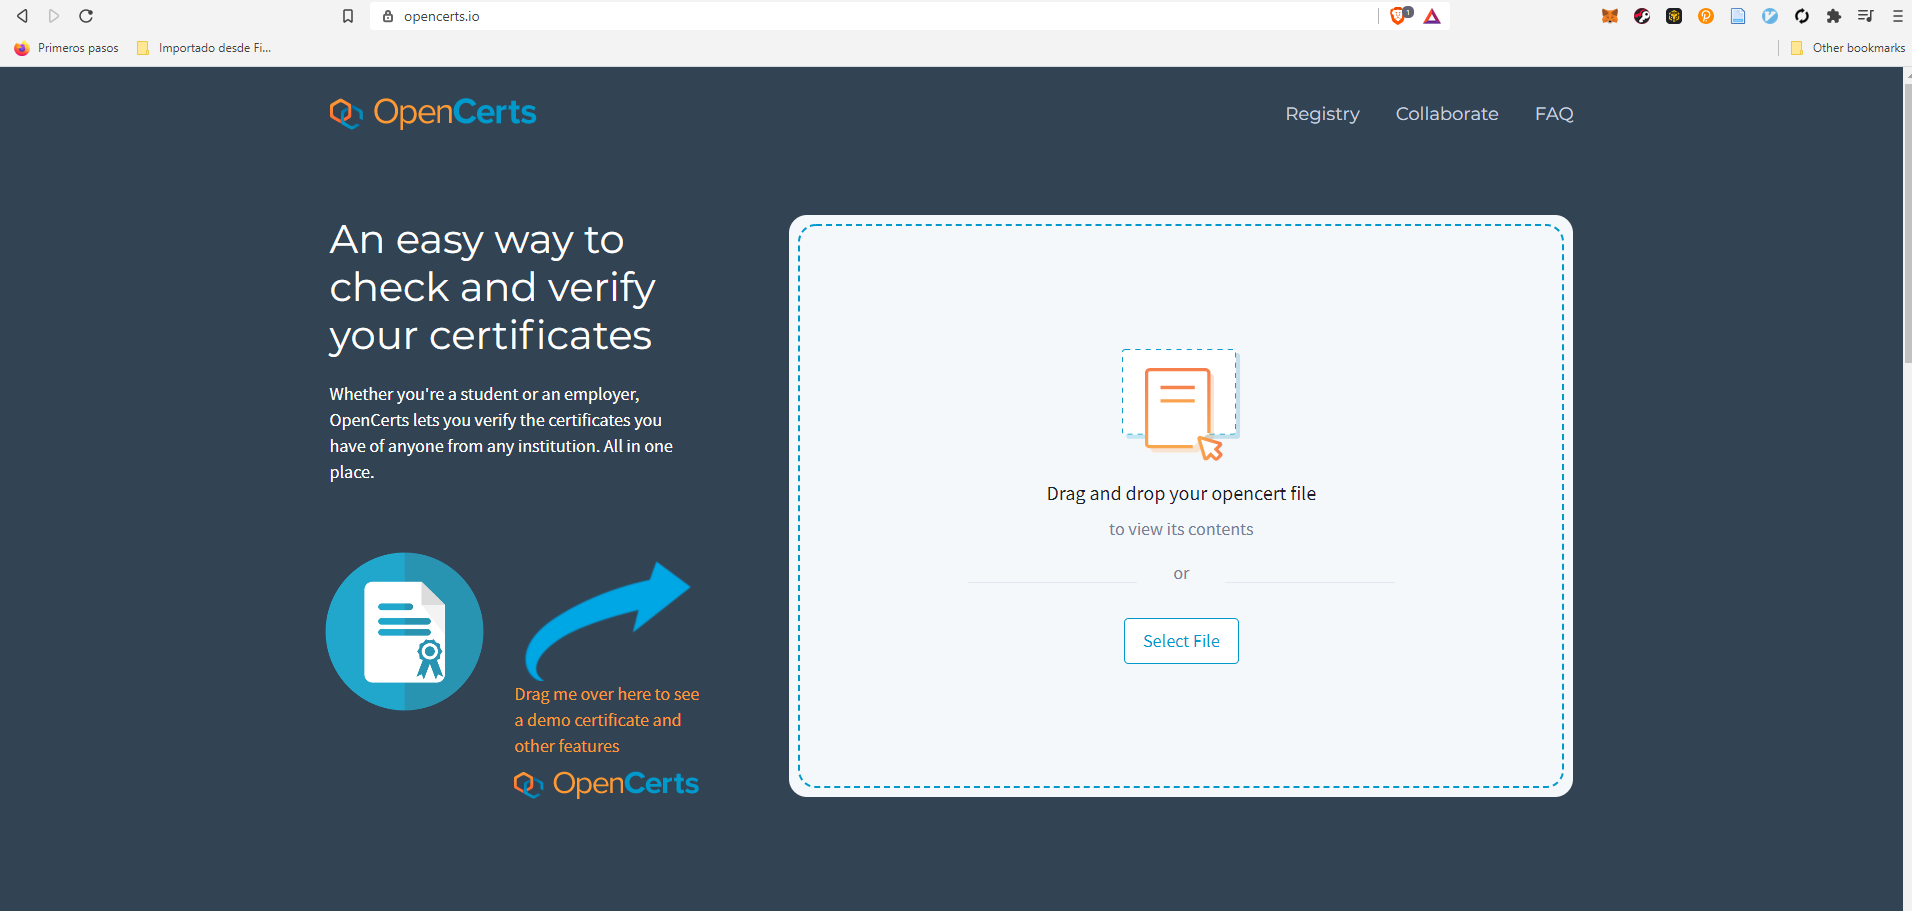
\includegraphics[scale=0.3]{OpenCerts_Home.png}}
  \caption{Página Web de OpenCerts}
  \label{img:opencerts_home}
\end{figure}

En la imagen \ref{img:opencerts_home} se puede observar lo sencillo que es verificar un documento. Simplemente se arrastra el  archivo 
de extensión“.opencerts”
y se buscará en la  Blockchain si realmente fue emitido por alguna entidad.
OpenCerts utiliza los smart contract en la  Blockchain de Ethereum. También utiliza tecnologías como Ract.js, Metamask, Web3.js, entre otros. 
Lo que permite desarrollar
un sistema de certificados totalmente descentralizado \cite[]{opencerts_gestion_nodate}. 
\subsection{BlockCerts}
Se define a si mismo 
como un estándar abierto   desarrollado por el MIT Media Lab y Learning Machine, para la construcción  de  aplicaciones que emiten y verifican registros oficiales basados
en la Blockchain. Pueden incluir certificados de registros civiles, académicos, licencias profesionales y más. 
Consiste en una librería con herramientas y apps móviles habilitando un ecosistema descentralizado, basado en estándar y habilitando verificación sin necesidad de la confianza mediante la tecnología  Blockchain \cite[]{blockcerts_introduction_nodate}.
Algunas universidades como el Instituto Tecnológico de Massachusetts (MIT), Tecnológico de Monterrey, la Universidad Harvard, la Universidad de California en Berkeley lo aplican. El 
estándar plantea que los certificados puedan ser compatibles a un nivel global, sin importar
la  Blockchain que se utilice pudiendo ser Bitcoin, Ethereum u otra \cite[]{edublocs_nueve_2019,criptomonedas_tv_entrevista_2018}. 

\begin{figure}[H]
  \centering
  {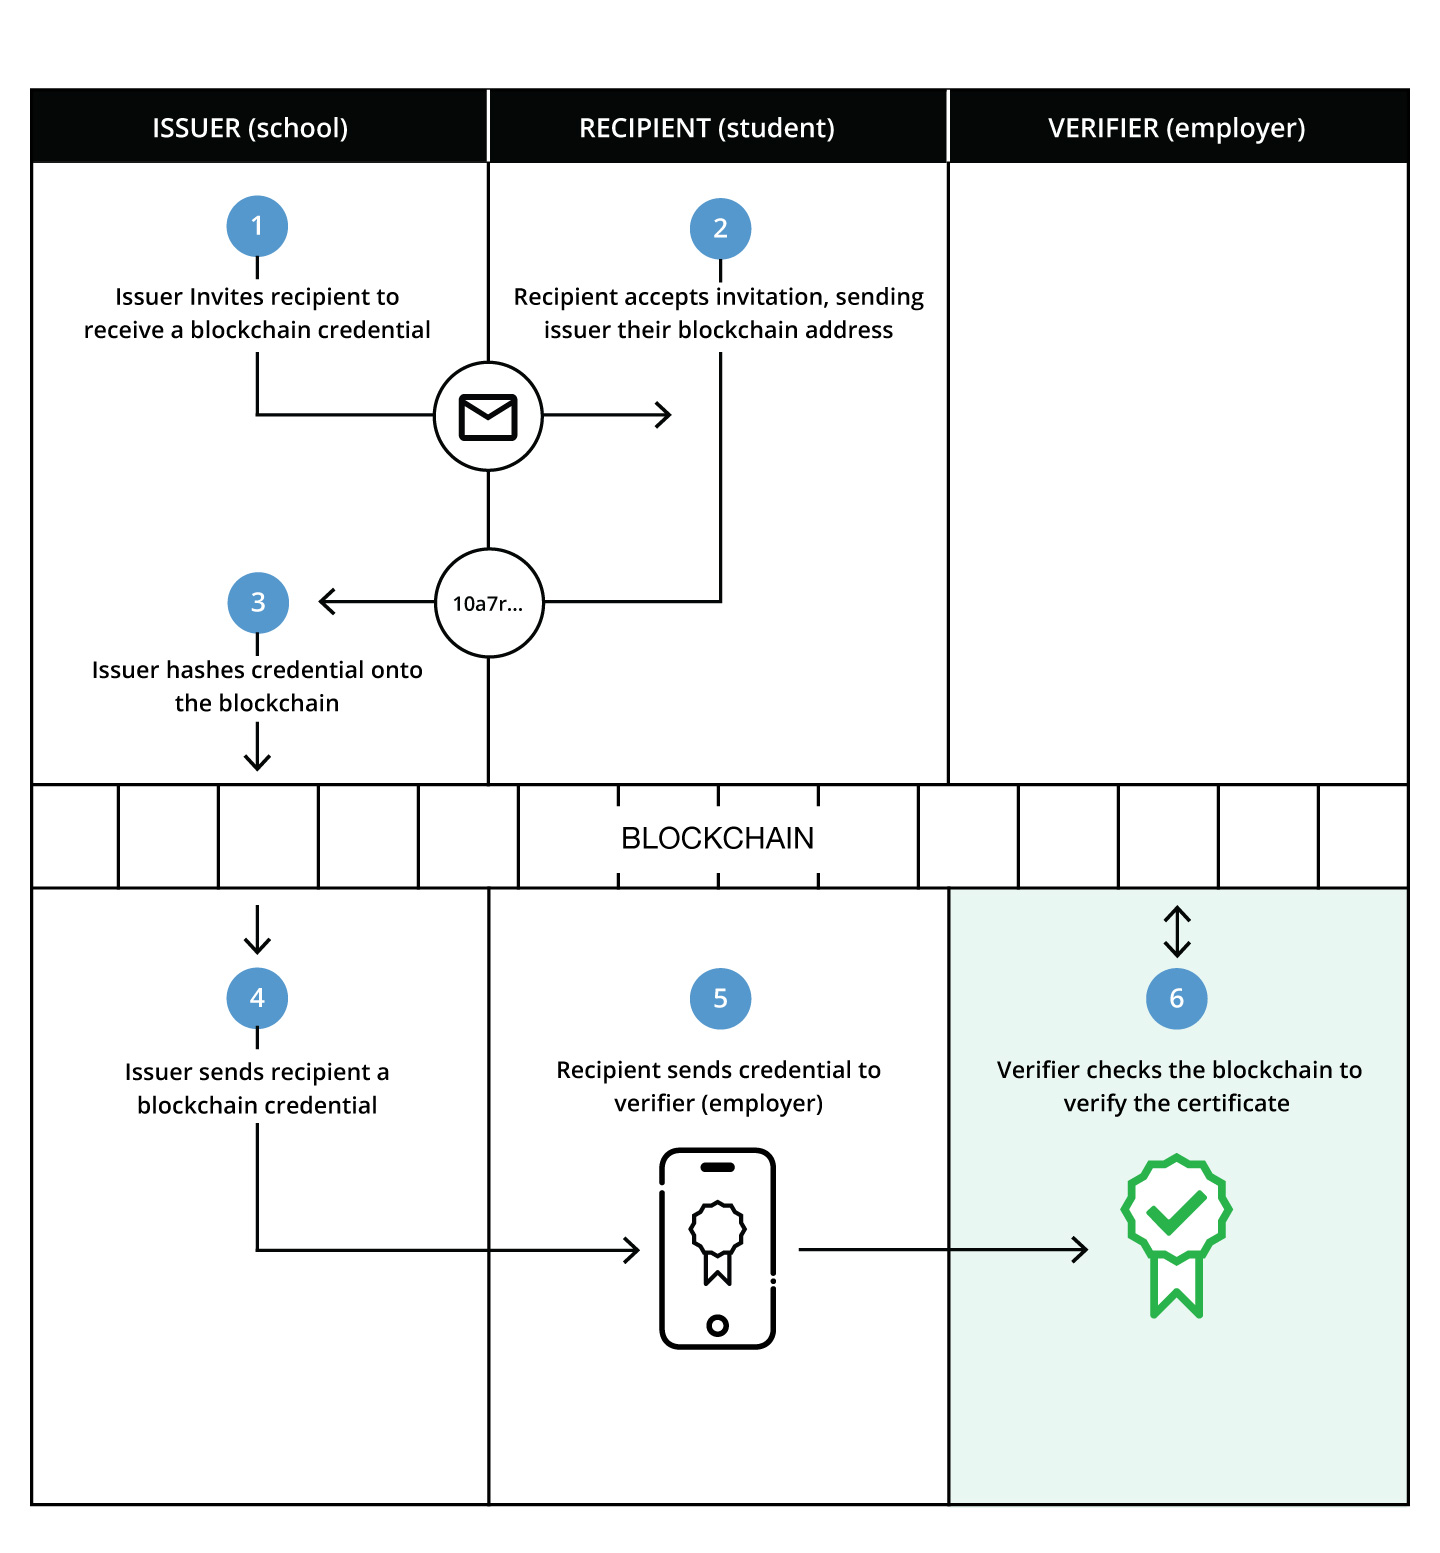
\includegraphics[scale=0.3]{blockcerts_how_it_works.jpg}}
  \caption{Imagen extraída de la página oficial de BlockCerts}
  \label{img:blockcerts_how_it_works}
\end{figure}

El flujo básico que se visualiza en  la figura \ref{img:blockcerts_how_it_works}   para comprobar que
un certificado se encuentra almacenado en la  Blockchain y es validado por un instituto se explica a continuación:

En el paso 1, el emisor o institución invita a un usuario a que brinde su dirección de cuenta o su clave pública creada 
descargando, la aplicación movil que provee BlockCerts. En el paso 2, el usuario envía al emisor su clave pública.
El paso 3 y 4, el emisor crea el hash a partir del certificado y lo almacena en la  Blockchain para luego enviar un archivo de tipo JSON 
\footnote{JavaScript Object Notation es un formato basado en texto estándar para representar datos estructurados \cite[]{mozilla_trabajando_json}.}, que contiene
la información sobre el documento del estudiante o dueño del certificado. En el paso 5, puede enviar este documento a cualquier empresa o individuo que desee.
 En el paso 6 el usuario que posee el archivo puede verificarlo en el sitio web de  BlockCerts \cite[]{blockcerts_introduction_nodate}.

 



 

%------------------ Antecedentes y tendencias --------------------
%% antecedentes de certificados digitales con  Blockchain y si existe alguna moda o tendencia actual.
\chapter{Antecedentes y Tendencias}
En el capítulo actual se exponen los antecedentes de la tecnología  Blockchain utilizándola como soporte para 
la validación, así como las tendencias del uso de la tecnología en distintos niveles como el internacional, nacional y local.

\section{Nivel Internacional}

\subsection{Antecedentes}
Tras la presentación de Bitcoin a partir del año 2008 \cite[]{alice_blockchain_2021}, como una solución al problema del doble gasto y un medio de pago puramente electrónico \cite[]{nakamoto_bitcoin_2008},
surgen copias de esta red con mejoras en cuanto a la escalabilidad y velocidad de transacciones. Cuando Ethereum hizo presencia  con
un enfoque diferente a Bitcoin, expande el uso de la Blockchain
con la incorporación de los smart contract \cite[]{ethereum_que_2020}.  %Estos son programas alojados en la Blockchain,
No tardaron en surgir otras  Blockchain similares a la de Ethereum, como EOS, 
NEO,  cada una de ellas  tiene su particularidad en sus objetivos, la manera de utilizarlos y sus protocolos.

Desde el surgimiento de Ethereum, se  desarrollaron aplicaciones que permiten
representar activos del mundo real, siendo estos: títulos de automotores, terrenos o propiedades inmuebles,
títulos académicos, u otros instrumentos que representen valores para las personas.
Desde el despliegue de Ethereum 1.0 en el año 2015 se crearon  aplicaciones de video juegos,
financieras, redes sociales, arte digital, entre otros. El mundo del  Blockchain es un mar de proyectos e innovaciones,
por ende se hará foco en el área de educación académica, especialmente
en la validación de certificados, títulos o documentaciones relacionadas a esta
área \cite[]{drescher_Blockchain_2017,cheng_Blockchain_2018}.



La tecnología Blockchain es muy utilizada en la administración pública en países como Estonia, 
donde tienen un modelo de gobierno electrónico que es la identidad digital, con ella los estonios tienen sus datos
que lo identifican electrónicamente, permite  acceder a servicios del pais y viajar por la Unión Europea.   
Tienen un sistema de ciudadanía e-Residenc que permite a los extranjeros  viajar a distintos países con su
registro digital. Usan sus documentos de identidad electrónica para editar y revisar 
documentos fiscales, solicitar beneficios de seguridad social y obtener servicios bancarios \cite[]{brys_cadena_2019}.

Estonia no es el único país que se beneficia de la tecnología  Blockchain. Ucrania usa un sistema 
eAuction 3.0, usado para el alquiler o ventas de bienes del Estado para combatir 
la corrupción y disminuir la burocracia.
En Suecia hay un proyecto que permite almacenar transacciones inmobiliarias
de forma que todas las contrapartes: los bancos, los agentes, los compradores y vendedores  pueden 
tener la oportunidad de seguir el proceso de la implementación del acuerdo después de su finalización.
También  Georgia, Grecia y Honduras aplican la tecnología
Blockchain \cite[]{brys_cadena_2019}.

\subsection{Tendencias}


 La Blockchain  es utilizado cada día  por distintos sectores para respaldar 
documentos, así también en casos de agricultura, y cada vez surgen nuevos proyectos \cite[]{Blockchain_federal_argentina_trazabilidad_nodate}. 

Actualmente el mundo del  Blockchain está en crecimiento con los proyectos relacionados a los 
criptoactivos, ya que la gran mayoría de los consumidores de esta tecnología lo usan para generar ingresos con las distintas manera que  ofrecen los proyectos.
Existen sistemas web que publican las criptoactivos con mayor relevancia según el relevamiento que realizan ellos, 
dos de estos sistemas web son CoinMarketCap y CoinGecko.

Durante el desarrollo de la investigación, mediante  la utilización de la herramienta Google Trends,
se compararon los términos de búsquedas  Bitcoin, Ethereum, Blockchain, DApp y Cryptocurrency, desde  la figura  \ref{img:google_trends} 
 se puede observar según la tabla de interés que genera la herramienta en un rango de 0 a 100, donde Bitcoin es el 
término de búsqueda más popular inclusive que la Blockchain y el término Cryptocurrency o Criptomoneda. En comparación con la búsqueda DApp esta última
no parece ser muy conocida.  


\begin{figure}[H]
    \centering
    {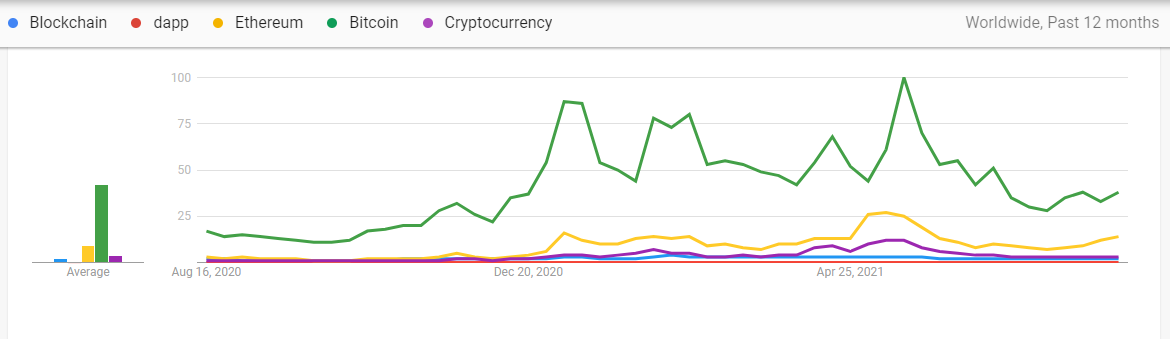
\includegraphics[scale=0.4]{google_trends.png}}
    \caption{Captura de pantalla de la  página Google Trends el dia 11/08/2021 } 
    \label{img:google_trends}
\end{figure}

En el mundo de la Blockchain las recientes tendencias fueron el uso de las Finanzas Descentralizadas (DeFi) y 
los Token No Fungibles (NFT). Las DeFi son muy consumidas en las últimas fechas por el retorno
de inversión que obtienen los usuarios a depositar sus criptoactivos. Y por el otro lado los NFTs
son unos criptoactivos que permiten representar la posesión de un elemento en particular, por ejemplo,
una obra de arte digital se puede comprar en el ecosistema de Blockchain, pero solo unos pocos usuarios serían dueños de ellos 
por en la escasez de ellos hacen que los NFT se han vendido a precios elevados \cite[]{brys_cadena_2019,cripto247_2021_2021}.


\section{Casos en Argentina}
\subsection{Antecedentes}


La \gls{bfa} \footnote{\href{https://bfa.ar/}{bfa.ar}} se describe a sí misma como una plataforma multiservicios, abierta y participativa, pensada para integrar servicios y aplicaciones 
sobre Blockchain.
Una iniciativa confiable y auditable que permita optimizar procesos y funcione como herramienta de empoderamiento para toda la comunidad
\cite[]{Blockchain_federal_argentina_que_nodate}.
Sobre esta plataforma se han creado diversas aplicaciones de distintos ámbitos como la publicación de documentos como el {Boletín Oficial de la República Argentina}, de empresas privadas, también aplicaciones de trazabilidad, y otras que se pueden relacionar a:
\begin{enumerate}
  
  \item El Ministerio de Educación, Cultura, Ciencia y Tecnología cuenta con el Registro Público de Graduados Universitarios que proporciona datos de egresados universitarios certificados por el Ministerio de Educación de toda la República Argentina. Gracias a la digitalización del trámite de certificación de diplomas y analíticos, y a la incorporación de  Blockchain  en el proceso, es posible autenticar la veracidad de la información contenida en el registro y que ésta sea accesible a la comunidad \cite[]{Blockchain_federal_argentina_aplicaciones_nodate}.
  
  \item  Sistema de Información Universitario (SIU). El SIU-Diaguita como el  Módulo de Compras y el de  Contrataciones y Patrimonio del SIU, son utilizados por más de 50 Universidades Nacionales y Organismos Públicos. Se incorporó el uso de  la \gls{bfa} a través  de la funcionalidad de recepción de ofertas. De esta manera, las fechas y horas de las ofertas de los proveedores  se registran en el sistema y queda certificada en la Blockchain 
\cite[]{Blockchain_federal_argentina_aplicaciones_nodate}.

\item En la Universidad Nacional de Córdoba gracias a la digitalización de los sistemas de gestión de alumnos utilizados en universidades para la carga y archivo de actas de examen, promoción y equivalencia, entre otros datos, es posible verificar dicha información por medio de  Blockchain, y garantizar al alumnado, personal administrativo y autoridades de las unidades académicas, que el sistema no puede presentar alteraciones en los registros sin que esas modificaciones sean detectadas \cite[]{Blockchain_federal_argentina_aplicaciones_nodate}.
\end{enumerate}


\subsection{Tendencias}
Por otro lado el gobierno Argentino impulsa un proyecto de ley relacionada a las criptomonedas y activos digitales,
el objetivo es crear un marco regulatorio integral, aplicable a las transacciones y operaciones civiles y 
comerciales de criptoactivos  y permitir
el crecimiento del ecosistema local  \cite[]{dagostino_exclusivo_nodate}.

El artículo describe que la promulgación de esta ley permitirá:
\begin{enumerate}
    \item El Estado pueda determinar qué \glsplural{proyecto_cripto} autoriza y cuáles no en base criterios legales que hoy no existen.

    \item Las empresas tengan modelos de negocios que cumplan con ciertos criterios, como una  Blockchain pública o casos de uso.

    \item Se puedan representar tenencias de acciones, una propiedad, etcétera.

\end{enumerate}

La definición de un criptoactivo posibilitará que las capitales de riesgos internacionales 
que pretenden invertir tengan  seguridad jurídica y la certeza destinado los fondos \cite[]{dagostino_exclusivo_nodate}. 


\section{Casos en Misiones}
\subsection{Antecedentes}

El proyecto Colmena está basado en la participación ciudadana para recuperar residuos y generar un nuevo modelo económico 
que recompensa a los ciudadanos con la criptomoneda JellyCoin por sus aportes a partir del aprovechamiento de los residuos. 
Iván Zubilewicz, director del Proyecto Colmena, explicó que es un modelo para recuperar 
los residuos a través de una economía colaborativa con la tecnología Blockchain. El modelo
integra al usuario que quiere recuperar los materiales residuales por medio de la plataforma y el recolector 
puede visualizar los residuos que la comunidad acumula para luego transportarlo a los emprendimientos industriales.
El modelo permite incentivar al ciudadano a cuidar el medio ambiente y a su vez obtener JellyCoin, la cual las empresas
deberán utilizar para comprar los residuos recolectados y formar un circuito de economía con la criptomoneda como muestra la figura \ref{img:colmena-movida}
extraída de la página noticiasdel6.com Proyecto Colmena: un modelo de recuperación de residuos \cite[]{noticiasdel6com_proyecto_2020,jimenez_proyecto_2020}. 

\begin{figure}[H]
    \centering
    {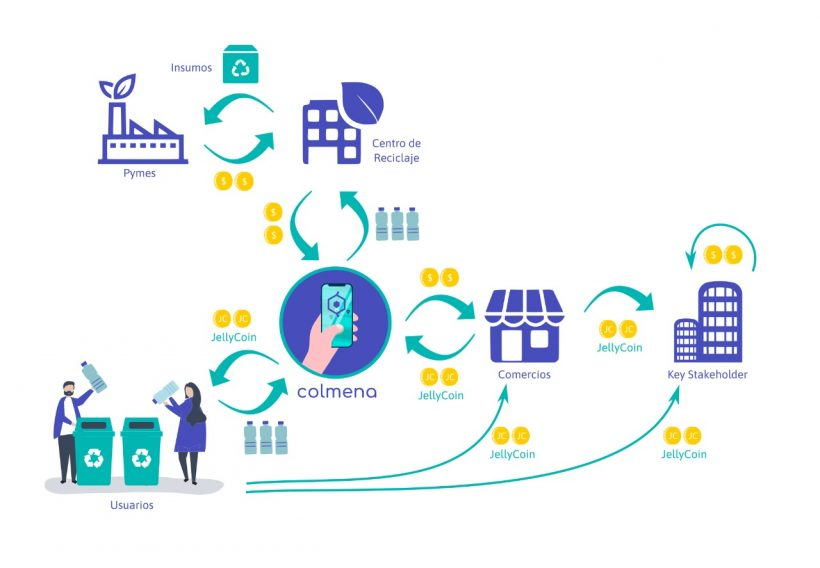
\includegraphics[scale=0.7]{colmena-movida.jpg}}
    \caption{Modelo del Proyecto Colmena extraída de la página noticiasdel6.com} 
    \label{img:colmena-movida}
\end{figure}

\subsection{Tendencias}

La Cámara de Diputados de la Provincia de Misiones de Argentina aprobó el proyecto denominado como 
Programa Misionero de Innovación Financiera con Tecnología Blockchain y Criptomoneda \cite[]{camara_de_representantes_de_la_provincia_de_misiones_programa_2020}. A partir del proyecto
la Provincia podrá emitir su propia Criptomoneda y almacenar datos de la administración pública en la Blockchain.
Los objetivos principales son emitir una propia StableCoin (Moneda Estable) que usará la Provincia como herramienta de financiación entre el sector público
y privado, otro uso es la gestión de datos para la administración pública y por último la emisión de certificados verdes con el uso de la tecnología 
usarlo para validar títulos o certificados \cite[]{clementin_provincia_2021}. 

% \section{Tendencias}

% \subsection{Diplomas Digitales Argentina }
% Las certificaciones digitales del ámbito académico aumentaron su uso en el último tiempo; un ejemplo de ello es  
% la Universidad de Buenos Aires (UBA), que expide sus títulos por un sistema online que acorta el tiempo 
% a dos meses generando un documento digital de  formato pdf encriptado. En el sitio web describen que los diplomas digitales 
% corresponden a carreras  de grado, acreditaciones parciales de una carrera de grado, carreras técnicas de nivel universitario, de 
% complementación curricular de una carrera de grado y  de posgrado también certificados de reválida expedidos 
% por la Universidad y certificados analíticos finales \cite[]{facultad_de_farmacia_y_bioquimica_universidad_de_buenos_aires_diploma_2020}.

% Asi mismo el Rectorado de la UBA, dispuso mediante la Resolución {RESCS}-2020-271-{E}-{UBA}-{REC}\cite[]{universidad_de_buenos_aires_resolucion_2020}  
% Define que "Los diplomas serán firmados digitalmente con dispositivo
% criptográfico por el o la Rectora y el o la Secretaria de Asuntos Académicos de esta
% Universidad; la/s o lo/s Decano/s y el o la Secretaria/s Académica/s de la/s
% Facultad/es. El Director o Directora General de la Dirección General de Títulos y
% Planes certificará con su firma digital toda la información que deba constar de
% acuerdo con el tipo de diploma expedido.
% Sin perjuicio de su firma digital, en el anverso de los diplomas se reproducirán las
% firmas ológrafas y se consignará los nombres, apellidos y cargo de las autoridades
% indicadas en el párrafo precedente. En el reverso, se reproducirá la firma ológrafa
% del Director o Directora General de la Dirección General de Títulos y Planes."\cite[]{universidad_de_buenos_aires_anexo1_2020}

% De esta forma, se observa que la universidad utiliza el método de firma digital para asegurar la integridad de los documentos digitales.
% En la resolución mencionada se muestran los modelos de los certificados y son considerados documentos digitales en sí. La Figura \ref{img:modelo1-certificado}  representa el 
% Modelo 1, este documento corresponde a una carrera técnica de nivel universitario o carrera de grado completa 
% dependiente de un Facultad  \cite[]{universidad_de_buenos_aires_anexo2_2020}. 

% \begin{figure}[hbt!]
%     \centering
%     {
\includegraphics[scale=0.7]{modelo1-certificado.png}}
%     \caption{Modelo 1 de Certificado} 
%     \label{img:modelo1-certificado}
% \end{figure}


% Los certificados digitales también son utilizados en  la Universidad Nacional De La Plata (UNLP) 
%  ya que la entrega de los títulos es completamente online y los primeros en recibirlos
% fueron estudiantes de la Licenciatura en Sistemas. El proceso de emisión del  título  hasta que lo reciben los egresados de las 
% carreras ha mejorado significativamente, ya que  testimonios de esperar 
% meses los títulos ahora lo reciben en cuestiones de días \cite[]{unlp_certificado_2020}.


% En cuanto a las tendencias de la tecnología Blockchain, resaltan 
% la creación de proyectos relacionados al ámbito financiero, mientras que en otras áreas como identidad digital, votos, sectores académicos 
% se la utiliza pero siguen siendo más consultada y en cantidad el uso financiero como creación
% de monedas digitales y ecosistemas que permiten a las personas utilizarlos.\cite[]{preukschat_Blockchain_2018,drescher_Blockchain_2017}

% \subsection{Las Tecnologías Digitales }
 La Blockchain  cada día es utilizado por distintos sectores para respaldar 
documentos, asi también en casos de agricultura, y cada vez se muestran nuevos proyectos \cite[]{Blockchain_federal_argentina_trazabilidad_nodate}. 

Actualmente el mundo del  Blockchain está en crecimiento con los proyectos relacionados a los 
criptoactivos, la gran mayoría de los consumidores de esta tecnología lo usan para generar 
ganancias o ingresos con las distintas manera que  ofrecen los proyectos.
Existen sistemas web que públican las criptoactivos con mayor relevancia según el relevamiento que realizan ellos, 
dos de estos sistemas web son CoinMarketCap y CoinGecko.

% \begin{figure}[hbt!]
%     \centering
%     {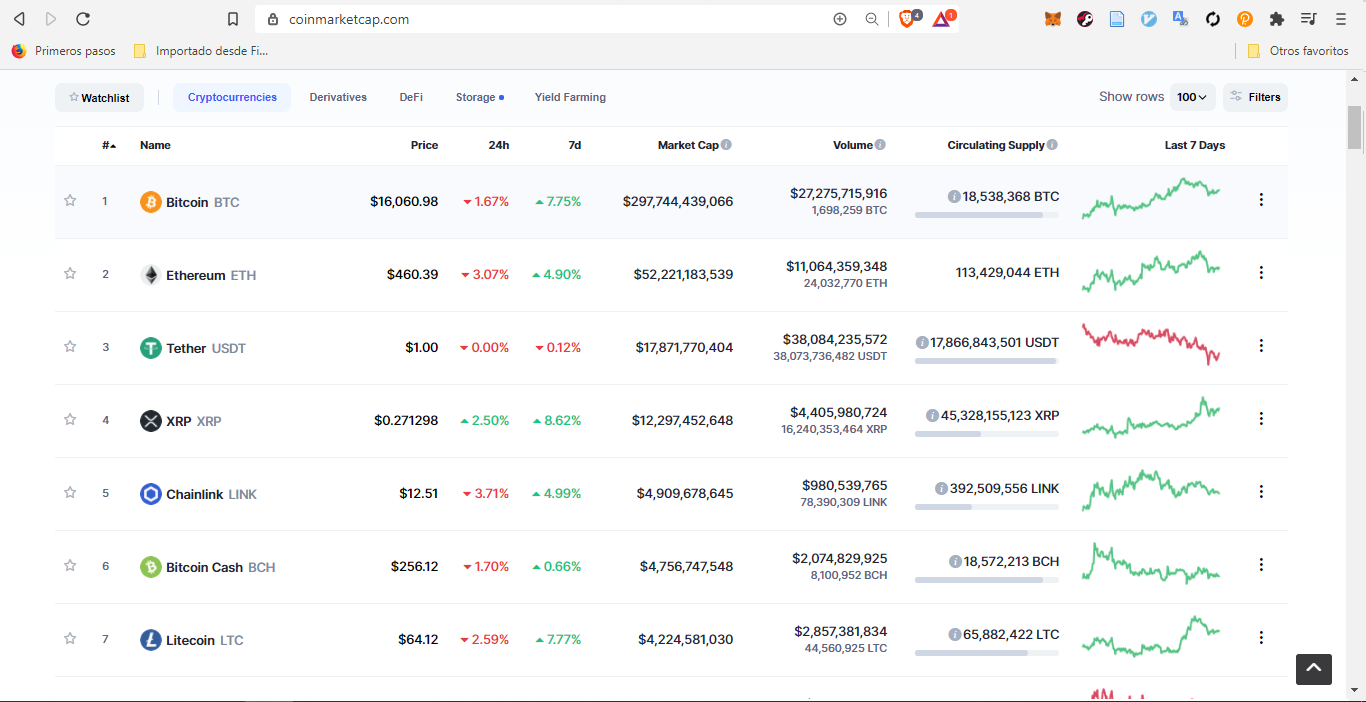
\includegraphics[scale=0.4]{coinmarketcap-valores.png}}
%     \caption{Captura de pantalla de la  página CoinMarketCap el 14/11/2020 a las 21:23 hs Argentina} 
%     \label{img:coinmarketcap-valores}
% \end{figure}

% \begin{figure}[hbt!]
%     \centering
%     {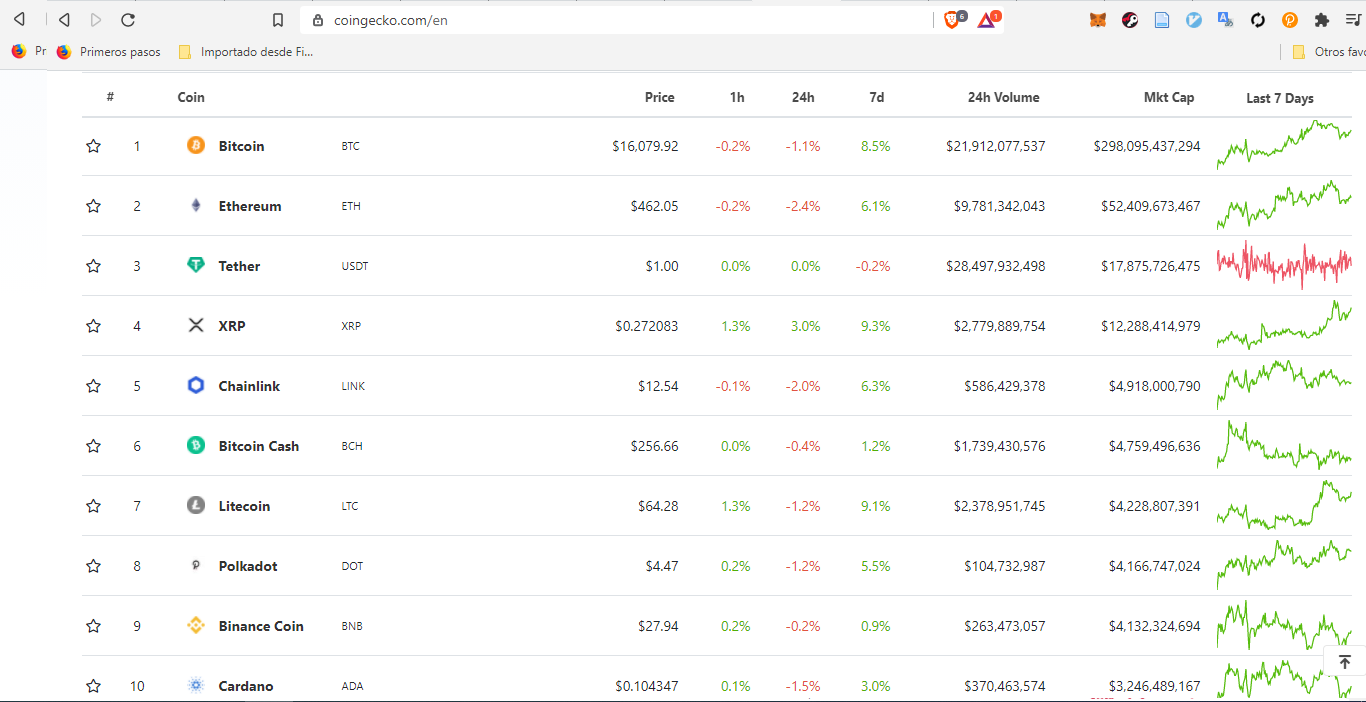
\includegraphics[scale=0.4]{coingecko-valores.png}}
%     \caption{Captura de pantalla de la  página CoinGecko el 14/11/2020 a las 21:23 hs Argentina} 
%     \label{img:coingecko-valores}
% \end{figure}

% En la  Figura \ref{img:coinmarketcap-valores} 
%  y 
% Figura \ref{img:coingecko-valores}     
% muestra una lista de los criptomonedas y los tokens con mayor capital de mercados.
Generalmente los  dos primeros puestos se están Bitcoin (BTC) y el Ether (ETH) que son criptomonedas nativa de su Blockchain. 
Asi como estas monedas digitales existen un sin numero de ellas y se crean constantemente, donde su valor reside en la oferta y demanda,
si no hay demanda por la obtención de un activo digital, no tiene valor \cite[]{joaquin_lopez_lerida_economiBlockchain_2016}.

Por otro lado el gobierno Argentino impulsa un proyecto de ley relacionadas a las criptomonedas y activos digitales,
el objetivo es crear un marco regulatorio integral, aplicable a las transacciones y operaciones civiles y 
comerciales de criptoactivos  y permitir
el crecimiento del ecosistema local  \cite[]{dagostino_exclusivo_nodate}.


El artículo \cite[]{dagostino_exclusivo_nodate} describe que la promulgación de esta ley permitirá:
\begin{enumerate}
    \item El Estado pueda determinar qué \glsplural{proyecto_cripto} autoriza y cuáles no en base criterios legales que hoy no existen.

    \item Las empresas tengan modelos de negocios que cumplan con ciertos criterios, como una  Blockchain pública o casos de uso.

    \item Se puedan representar tenencias de acciones, una propiedad, etcétera.

\end{enumerate}


La definición de un criptoactivo posibilitará que las capitales de riesgos internacionales 
que pretenden invertir tengan  seguridad jurídica y la certeza destinado los fondos \cite[]{dagostino_exclusivo_nodate}. 

% Esto no es nuevo, en países como EE.UU., China, Rusia se 
% encuentran operando con monedas digitales gubernamentales y expresan que será un punto de partida para crear nuevos servicios y obtener un liderazgo a nivel regional
% como global \cite[]{dagostino_exclusivo_nodate}.

La Cámara de Diputados de la Provincia de Misiones de Argentina aprobó el proyecto denominado como 
Programa Misionero de Innovación Financiera con Tecnología Blockchain y Criptomoneda. A partir del proyecto
la Provincia podra emitir su propia Criptomoneda y almacenar datos de la administración pública en la Blockchain.
Los objetivos principales son emitir una propia StableCoin (Moneda Estable) que usara la Provincia como herramienta de financiación entre el sector público
y privado, otro uso es la gestión de datos para la administración pública y por último la emisión de certificados verdes con el uso de la tecnología 
usarlo para validar titulo o certificados. \cite[]{clementin_provincia_2021}



% \section{Tendencias}

% \subsection{Diplomas Digitales Argentina }
% Las certificaciones digitales del ámbito académico aumentaron su uso en el último tiempo; un ejemplo de ello es  
% la Universidad de Buenos Aires (UBA), que expide sus títulos por un sistema online que acorta el tiempo 
% a dos meses generando un documento digital de  formato pdf encriptado. En el sitio web describen que los diplomas digitales 
% corresponden a carreras  de grado, acreditaciones parciales de una carrera de grado, carreras técnicas de nivel universitario, de 
% complementación curricular de una carrera de grado y  de posgrado también certificados de reválida expedidos 
% por la Universidad y certificados analíticos finales \cite[]{facultad_de_farmacia_y_bioquimica_universidad_de_buenos_aires_diploma_2020}.

% Asi mismo el Rectorado de la UBA, dispuso mediante la Resolución {RESCS}-2020-271-{E}-{UBA}-{REC}\cite[]{universidad_de_buenos_aires_resolucion_2020}  
% Define que "Los diplomas serán firmados digitalmente con dispositivo
% criptográfico por el o la Rectora y el o la Secretaria de Asuntos Académicos de esta
% Universidad; la/s o lo/s Decano/s y el o la Secretaria/s Académica/s de la/s
% Facultad/es. El Director o Directora General de la Dirección General de Títulos y
% Planes certificará con su firma digital toda la información que deba constar de
% acuerdo con el tipo de diploma expedido.
% Sin perjuicio de su firma digital, en el anverso de los diplomas se reproducirán las
% firmas ológrafas y se consignará los nombres, apellidos y cargo de las autoridades
% indicadas en el párrafo precedente. En el reverso, se reproducirá la firma ológrafa
% del Director o Directora General de la Dirección General de Títulos y Planes."\cite[]{universidad_de_buenos_aires_anexo1_2020}

% De esta forma, se observa que la universidad utiliza el método de firma digital para asegurar la integridad de los documentos digitales.
% En la resolución mencionada se muestran los modelos de los certificados y son considerados documentos digitales en sí. La Figura \ref{img:modelo1-certificado}  representa el 
% Modelo 1, este documento corresponde a una carrera técnica de nivel universitario o carrera de grado completa 
% dependiente de un Facultad  \cite[]{universidad_de_buenos_aires_anexo2_2020}. 

% \begin{figure}[hbt!]
%     \centering
%     {
\includegraphics[scale=0.7]{modelo1-certificado.png}}
%     \caption{Modelo 1 de Certificado} 
%     \label{img:modelo1-certificado}
% \end{figure}


% Los certificados digitales también son utilizados en  la Universidad Nacional De La Plata (UNLP) 
%  ya que la entrega de los títulos es completamente online y los primeros en recibirlos
% fueron estudiantes de la Licenciatura en Sistemas. El proceso de emisión del  título  hasta que lo reciben los egresados de las 
% carreras ha mejorado significativamente, ya que  testimonios de esperar 
% meses los títulos ahora lo reciben en cuestiones de días \cite[]{unlp_certificado_2020}.


% En cuanto a las tendencias de la tecnología Blockchain, resaltan 
% la creación de proyectos relacionados al ámbito financiero, mientras que en otras áreas como identidad digital, votos, sectores académicos 
% se la utiliza pero siguen siendo más consultada y en cantidad el uso financiero como creación
% de monedas digitales y ecosistemas que permiten a las personas utilizarlos.\cite[]{preukschat_Blockchain_2018,drescher_Blockchain_2017}

% \subsection{Las Tecnologías Digitales }
 La Blockchain  cada día es utilizado por distintos sectores para respaldar 
documentos, asi también en casos de agricultura, y cada vez se muestran nuevos proyectos \cite[]{Blockchain_federal_argentina_trazabilidad_nodate}. 

Actualmente el mundo del  Blockchain está en crecimiento con los proyectos relacionados a los 
criptoactivos, la gran mayoría de los consumidores de esta tecnología lo usan para generar 
ganancias o ingresos con las distintas manera que  ofrecen los proyectos.
Existen sistemas web que públican las criptoactivos con mayor relevancia según el relevamiento que realizan ellos, 
dos de estos sistemas web son CoinMarketCap y CoinGecko.

% \begin{figure}[hbt!]
%     \centering
%     {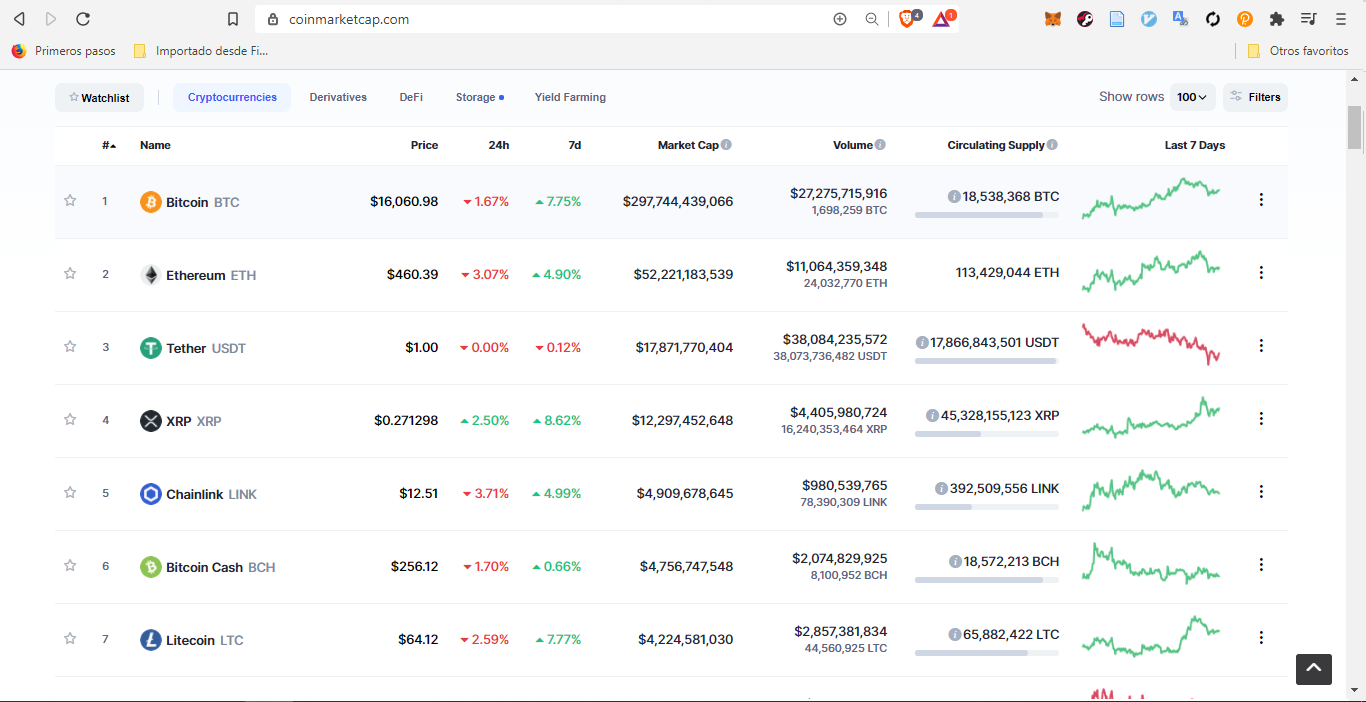
\includegraphics[scale=0.4]{coinmarketcap-valores.png}}
%     \caption{Captura de pantalla de la  página CoinMarketCap el 14/11/2020 a las 21:23 hs Argentina} 
%     \label{img:coinmarketcap-valores}
% \end{figure}

% \begin{figure}[hbt!]
%     \centering
%     {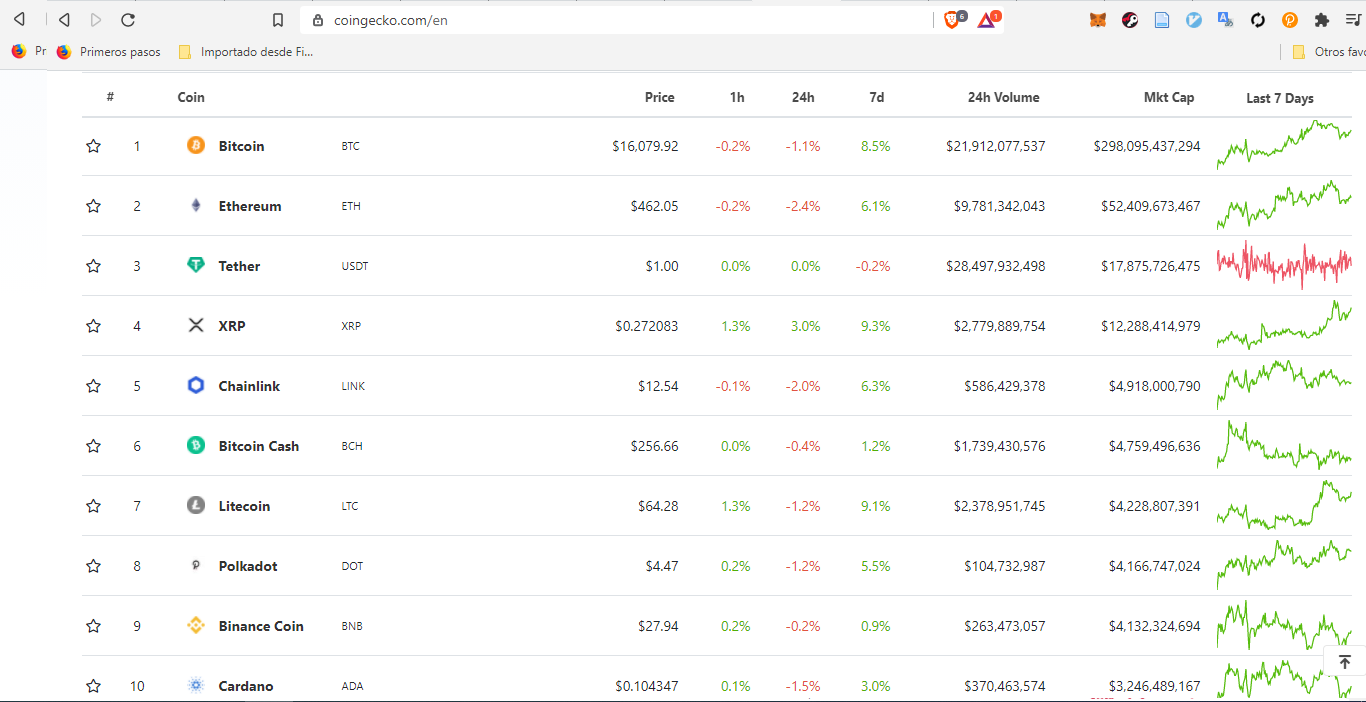
\includegraphics[scale=0.4]{coingecko-valores.png}}
%     \caption{Captura de pantalla de la  página CoinGecko el 14/11/2020 a las 21:23 hs Argentina} 
%     \label{img:coingecko-valores}
% \end{figure}

% En la  Figura \ref{img:coinmarketcap-valores} 
%  y 
% Figura \ref{img:coingecko-valores}     
% muestra una lista de los criptomonedas y los tokens con mayor capital de mercados.
Generalmente los  dos primeros puestos se están Bitcoin (BTC) y el Ether (ETH) que son criptomonedas nativa de su Blockchain. 
Asi como estas monedas digitales existen un sin numero de ellas y se crean constantemente, donde su valor reside en la oferta y demanda,
si no hay demanda por la obtención de un activo digital, no tiene valor \cite[]{joaquin_lopez_lerida_economiBlockchain_2016}.

Por otro lado el gobierno Argentino impulsa un proyecto de ley relacionadas a las criptomonedas y activos digitales,
el objetivo es crear un marco regulatorio integral, aplicable a las transacciones y operaciones civiles y 
comerciales de criptoactivos  y permitir
el crecimiento del ecosistema local  \cite[]{dagostino_exclusivo_nodate}.


El artículo \cite[]{dagostino_exclusivo_nodate} describe que la promulgación de esta ley permitirá:
\begin{enumerate}
    \item El Estado pueda determinar qué \glsplural{proyecto_cripto} autoriza y cuáles no en base criterios legales que hoy no existen.

    \item Las empresas tengan modelos de negocios que cumplan con ciertos criterios, como una  Blockchain pública o casos de uso.

    \item Se puedan representar tenencias de acciones, una propiedad, etcétera.

\end{enumerate}


La definición de un criptoactivo posibilitará que las capitales de riesgos internacionales 
que pretenden invertir tengan  seguridad jurídica y la certeza destinado los fondos \cite[]{dagostino_exclusivo_nodate}. 

% Esto no es nuevo, en países como EE.UU., China, Rusia se 
% encuentran operando con monedas digitales gubernamentales y expresan que será un punto de partida para crear nuevos servicios y obtener un liderazgo a nivel regional
% como global \cite[]{dagostino_exclusivo_nodate}.

La Cámara de Diputados de la Provincia de Misiones de Argentina aprobó el proyecto denominado como 
Programa Misionero de Innovación Financiera con Tecnología Blockchain y Criptomoneda. A partir del proyecto
la Provincia podra emitir su propia Criptomoneda y almacenar datos de la administración pública en la Blockchain.
Los objetivos principales son emitir una propia StableCoin (Moneda Estable) que usara la Provincia como herramienta de financiación entre el sector público
y privado, otro uso es la gestión de datos para la administración pública y por último la emisión de certificados verdes con el uso de la tecnología 
usarlo para validar titulo o certificados. \cite[]{clementin_provincia_2021}


 


%--------------- Situacion actual ------------------------------------
%%contar sobre como actualemte realizan la certificacion de los cursos de extension.
\chapter{Presentación del Caso} %% Analisis de como se trabaja en la UNAM Facultad de Extension.
%^%*************************************************************************
%% Presetacion 
%% Secretaría de extensión Que hacen, donde estan, que actividads realizan,.
%% Secretaría de extensión universitaria (SEU), (estatuto). 
\section{Contexto}

%Contar sobre la UNAM e ir acortando hasta llegar que la investigacion se realizara en laa Secretaria de extension de la Facultad de ciencias economicas.
% gestio documental dee la SE para cerrtificacion de documentos.
% explicar solo SE universitaria.

El estatuto describe a la \gls{unam} como una institución Universitaria de Derecho Público,
autónoma en lo académico e institucional y
autárquica en el sector económico y financiero. La institución 
tiene asiento en la provincia de Misiones de la República Argentina \cite[]{estatuto}. 

Impulsa la relación e integración con las instituciones afines,
gubernamentales y no gubernamentales de la provincia, regional,
nacional e internacional, que compartan o coincidan con sus fines 
y objetivos \cite[]{estatuto}.

Los fines de la \gls{unam} son descritos en el estatuto lo cual se
cita textualmente a continuación:

\begin{enumerate}
\item “La preservación promoción y difusión de la cultura universal con énfasis en lo nacional y
regional.”
\item “El resguardo acrecentamiento y difusión del conocimiento universal y del generado en su
propio ámbito.”
\item “La organización instrumentación y evaluación de la enseñanza-aprendizaje en los niveles de su
competencia y su articulación con los otros sectores del sistema educativo.”
\item “La aplicación del conocimiento a la solución de problemas del desarrollo humano en la provincia
, la región y el país.”
\item “El compromiso con la conservación y preservación del medio ambiente y los recursos naturales.”
\item “El de constituirse en un ámbito de formación ciudadana y ejercicio democrático.” \cite[]{estatuto}

\end{enumerate}

La \gls{unam} esta integrada por la \gls{fhycs}; \glsfirst{fce}; \gls{fceqyn}; \gls{fi} ; \gls{fayd};
\gls{fcf} 
\cite[]{estatuto}. Cada facultad de la \gls{unam} cuenta con las diferentes  Secretarías, Direcciones y Departamentos que necesiten gestionar información 
sobre los alumnos.

Prestando atención a las  secretarías las cuales varían sus nombres según la facultad, ellas son  la Secretaría Administrativa, 
Secretaría Académica, Secretaría de Investigación, Secretaría de Bienestar Estudiantil y Secretaría de Extensión.   

Todas  tienen en común  la gestión de  documentos y de información por ende deben generar nuevos documentos a partir de los 
hechos ocurridos, como ejemplo, la creación de un certificado de título académico por consecuencia de que un alumno de la facultad
finalizó el cien porciento (100\%) de su carrera. O la generación y gestión de cualquier otro documento que sea utilizado por 
la entidad como los planes de estudios, historia académica de los estudiantes, actas de exámenes, informes, entre otros (A.L., comunicación personal, 02/10/2020) \cite[]{estatuto}. 

% Se puede observar que en cada área de la universidad utilizan la gestión de información y documentación, es necesario por cuestiones 
% de optimización que la investigación límite el dominio en la cual sea aplicable el estudio por ello es recomendado realizarlo sobre un 
% área específica como la secretaría de extensión, la cual constantemente generan nuevos documentos \cite[]{larraburu_secretariextension_2020}.

La problemática que inicialmente impulsó la investigación es la validación de documentos relacionados a los estudiantes, sean certificados
o registros que puedan ser alterados. Dada la gran variedad de documentación que utiliza la universidad, se delimitó el alcance de la investigación en un área 
especifica, aún especificando un sector,
los documentos pueden ser variados, por lo tanto es necesario enfocarse en documentos relacionados a lo académico, con respecto a este tipo 
de documentación son considerados los que manejan datos de estudiantes, o participantes de eventos, excluyendo todo tipo de documentación 
relacionada al sector financiero  o asuntos administrativos (A.L., comunicación personal, 02/10/2020). %\cite[]{larraburu_secretariextension_2020}.

Las áreas seleccionadas para realizar la presente investigación son las Secretarías de Extensión de la \gls{unam} y sus respectivas facultades. 
Estas áreas tienen que gestionar documentaciónes de estudiantes y participantes de eventos por lo tanto, es un área adecuada para desarrollar el presente proyecto.

% las causas para la investigación pueden ser (relacionada a estadística) (por conveniencia explicar que solo se hace de una forma)

%% En la FCE se dictan carreras de gestion documental a la gestion. 
%  se presume (clave usar)



\section{Certificaciones de Actividades de Extensión en la \gls{fce} }
Las actividades universitarias de la \gls{unam} pretenden promover la interacción con el
medio en la cual integra, aportando al crecimiento social \cite[]{estatuto}. 

El estatuto \cite[]{estatuto} de la \gls{unam} describe que las actividades de extensión pueden implicar transferencia científico-tecnológica, 
educación permanente, difusión de actividades 
y producciones de la \gls{unam}, el desarrollo de las expresiones culturales y vinculaciones institucionales.




% \section{Secretaría de Extensión de la Facultad de Ciencias Económicas}

A un nivel jerárquico general está la  \gls{sgeu}, como lo define su nombre
es la secretaría general encargada de  gestionar y coordinar con las  secretarías de extensión de las distintas facultades \cite[]{estatuto}.

Por otra parte, la \gls{fce}  cuenta con su propia Secretaría 
de Extensión donde llevan a la práctica tareas como la generación de cursos, congresos, charlas, capacitaciones, eventos 
de cualquier características,
que permita cumplir con sus objetivos de expansión de conocimientos y crecimiento (A.L., comunicación personal, 02/10/2020).%\cite[]{larraburu_secretariextension_2020}.

El área administrativa de la Secretaría de Extensión es la encargada de realizar la gestión de las actividades que se planea efectuar.
Los eventos pueden ser iniciados por docentes, no docentes, funcionarios, secretarios o estudiantes pero el evento o actividad
debe  estar aprobada por algún instrumento.
Estos instrumentos pueden ser las disposiciones o resoluciones  que representan documentaciones que validan e impulsan 
la creación y ejecución de las actividades (A.L., comunicación personal, 02/10/2020).%\cite[]{larraburu_secretariextension_2020}.

Por otro lado, para que una actividad sea aprobada  es necesario que la 
propuesta tenga relación con los proyectos o programas planeados previamente. Esto quiere decir que las actividades deben estar justificadas y 
sus temas deben tener una relación estricta con los objetivos que la facultad propuso en sus proyectos o programas.
En el caso que se presente una propuesta de actividad que no se encuentra relacionado directamente a los proyectos o programas,
existe la posibilidad de presentarlo a las autoridades de la Secretaría de Extensión para evaluarlos y dictaminar su aprobación o rechazo (A.L., comunicación personal, 02/10/2020).% \cite[]{larraburu_secretariextension_2020}.

Una vez aprobada la actividad o el evento, el personal administrativo 
inicia con las preparaciones para relanzarlo. Se gestionan y reservan
las aulas necesarias o en caso que los participantes deban asistir 
físicamente una fecha y hora determinada, se prepara el registro
para quienes van dirigidos, ya que los eventos 
se realizan para un grupo selecto o también para todo el público interesado.
Se inicia toda la logística necesaria para el evento en particular (A.L., comunicación personal, 02/10/2020).%\cite[]{larraburu_secretariextension_2020}.

Para que los participantes de los eventos tengan un documento que constate
su presencia en las actividades,  se les entrega un certificado que dependiendo
de la situación son de asistencia al evento o exámenes aprobados (A.L., comunicación personal, 02/10/2020).%\cite[]{larraburu_secretariextension_2020}.

Depende de como se  organizó el evento y su magnitud, puede ocurrir que un evento
cuente con más de una charla y a su vez más de un curso. Por lo tanto
al planificar las actividades se opta cómo se entregarán los certificados:
uno por charla asistida o por asistencia total del evento sin detallar la actividad que realizó (A.L., comunicación personal, 02/10/2020).%\cite[]{larraburu_secretariextension_2020}. 

Los tipos de certificados académicos que se expiden en la secretaría de extensión de la \gls{fce}, son en formato papel, hojas tamaño A4 u oficio,
también certificados digitales como PDF e imágenes (A.L., comunicación personal, 02/06/2021).%\cite[]{larraburu_secretariextension_2020}. 



  
%^%*************************************************************************
\subsection{Proceso para Generar y Emitir  Certificados}

A continuación se describe el  proceso que se utiliza en la generación y emisión de los certificados 
relacionados a las actividades de la Secretaría de Extensión de la \gls{fce}; cabe aclarar que 
se explica el proceso para la certificación y no toda la gestión que se lleva a cabo
para que una actividad se realice. 

El proceso para la emisión y generación de los certificados para un evento está explicado en la entrevista de realizada al encargado de 
la Secretaría de Extensión de la \gls{fce} de la \gls{unam} (A.L., comunicación personal, 02/10/2020):%\cite[]{larraburu_secretariextension_2020} : 

\begin{enumerate}
    \item Días antes del evento se realiza el modelado de los certificados correspondiente a las actividades 
    que se planea realizar, dependiendo si los certificados serán solo por asistir al evento, se crea un modelo.
    Pero en el caso que se realice certificación por algún exámen aprobado o realizado, se crean 
    la cantidad de modelos de certificados según los exámenes a evaluar. 
  
    \item Una vez diseñados los modelos ideales para el evento se realiza el escaneo de las firmas de las autoridades de la facultad
    que representan a la institución académica, en este caso el secretario de extensión y otros responsables de ser necesarios.

    \item La firma escaneada de las autoridades se integra en los modelos de certificados, generando la documentación con la firma de las autoridades.


    \item El día del evento se registran los participantes que asisten, tomando los datos necesarios para los certificados.

    \item Al finalizar el evento se verifican los datos de las personas que se  registraron, y 
    las que asistieron a ellas. En este punto se determina quiénes de los participantes, recibirán 
    los certificados de asistencia.

    Con los datos de los participantes del evento se completan
    los certificados de asistencia de manera manual. Se agregaron los datos necesarios como 
    Apellido y Nombre, en otros casos otros datos extras como DNI, correo electrónico, 
    los datos del certificado dependerá de como se modeló el certificado.

    \item Cuando se finalizó con la carga de datos en los certificados de asistencias se entregan a los participantes.
    Depende de la planificación de la actividad, se entrega el certificado impreso en papel.
    O se envía el certificado digital por correo electrónico a cada participante.  
    
    
    
    \item Si la actividad contempla la certificación de aprobación de exámen, o 
    algún otro requerimiento específico. Se comprueba cuántos y quiénes de 
    los participantes  realizaron y aprobaron los requerimientos o el exámen.
   
    \item Una vez filtrados  los participantes que aprobaron los requerimientos o
    exámenes, se les crean manualmente (se ingresa el nombre y otros datos necesarios )
    el certificado perteneciente a cada participante que haya cumplido con las exigencias. 
    
    \item Finalizada la creación de los certificados de aprobación de exámen o 
    el requerimiento que se solicita para el certificado en particular se realiza
    la entrega del mismo modo que los certificados de asistencia. Mediante
    correo electrónico y en caso de ser físico, se contactan con los participantes para enviarles los certificados.
    
    Este último proceso de certificación se separa del certificado de asistencia.
    Porque de acuerdo al volumen de participantes y el criterio para evaluarlos, puede consumir más tiempo.
\end{enumerate} 

\subsection{Problemas Actuales}
Cuando  los participantes pretenden demostrar que asistieron o fueron parte de un evento de actualización, capacitación
o curso, ellos no tienen la manera de validar que sus documentos
digitales son los originales o si realmente fue emitido por la \gls{unam}, la única manera es con la impresión  del certificado 
y llevarlo a la Secretaría de Extensión de la \gls{fce} para  sellar  dando confirmación de que es un certificado emitido por la institución. Pero 
la validación de los mismos de manera digital no cuenta con un método definido para realizarlo (A.L., comunicación personal, 02/10/2020).%\cite[]{larraburu_secretariextension_2020}.

% En el caso que el participante desee demostrar que realizó los cursos, charlas o eventos específicos, la Secretaría de Extensión de la \gls{fce}
% debe hacerlo de manera física,  problema que no permite a los usuarios gestionar sus certificados digitales obtenidos a lo largo de todos los 
% eventos presenciados. 
% Las ventajas de realizar los certificados digitales es que el proceso de emisión y entrega es más rápido
% comparándolo al proceso físico a través de la impresión en soporte papel  de los certificados y entregándolo a cada uno de los participantes de los eventos.
% Mientras que la entrega de los certificados digitales se pueden hacer por otros medios más rápidos, como envío de correo electrónicos.

La Secretaría de Extensión de la \gls{fce} genera los certificados de manera física, lo sellan y entregan  físicamente; en los casos
que el participante de los eventos, charlas o cursos necesite demostrar que asistió a las actividades el 
proceso para validar sus certificados son lentos y con probabilidades de ser alterados. En comparación con
un proceso de validez digital que permite  ser automatizado, por lo tanto los medios de envíos son mas rápidos como por ejemplo
correos electrónicos y  brinda mayor velocidad en la validación de los certificados.
El método que utilizan para que los certificados digitales sean considerados válidos es incluir las firmas ológrafas de 
los responsables como el Secretario de Extensión o también los profesionales que son parte de la organización del evento, pero estas firmas
pueden ser copiadas y adaptadas a otros certificados de esta manera crear documentos que no fueron emitidos por la Secretaría de Extensión de la \gls{fce}.
Las entidades externas que desean averiguar si una persona realmente estuvo en el evento de interés, no tiene manera de 
comprobar la veracidad o autenticidad del certificado, por ende, el problema puede extenderse a dudar de la validez de los certificados (A.L., comunicación personal, 02/10/2020).%\cite[]{larraburu_secretariextension_2020}.
 


%------------------ Descripción del problema y solución--------------------
%% ser especifico cual es el problema y porque es un problema. Acordate que existe solucion para esto, pero no existe un sistema autonomo que certifique 

\chapter{Modelado de la Solución}
Como se mencionó en el capítulo anterior, el problema principal surge de la no utilización
de métodos que permitan validar los documentos digitales, emitidos por la Secretaría de Extensión de la \glsfirst{fce} de la \glsfirst{unam}.
En este capítulo se explica cómo abordar la solución a este problema.


Se propone un sistema que permita al usuario consultar la validez  de sus documentos digitales   por la entidad que los emitió
  y cuando se publicó, asimismo que permita a los gestores de la organizaciones subir  nuevos documentos o algún identificador  para comprobar
de manera inequívoca si fue emitido por ellos, aun cómo mostrar datos relacionados al evento de la institución u organización.
Con esta propuesta de sistema, se atenderían los aspectos mencionados en cuanto a las necesidades de brindar un medio por el cual
se pueda verificar que la documentación de las actividades desarrolladas por la  
Secretaría de Extensión de la \gls{fce} no fue adulterada, modificada o cambiada.


En cuestiones generales para solucionar los problemas se propone realizar un sistema que permita a la 
Secretaría de Extensión de la \gls{fce} de la \gls{unam} :

\begin{enumerate}
    \item Dar validez a un documento por tiempo determinado y gestionar sus estados.
    \item Definir qué entidades externas puedan validar la integridad de documentos digitales emitido por la Universidad.
    \item Permitir acceso a todo público al sistema para la validación.
    \item Proteger la privacidad de los datos que pertenecen a los documentos.
\end{enumerate}

A tales efectos los ítems recientemente expuestos se pueden lograr con la utilización de la tecnología Blockchain, 
otorgando inmutabilidad a los datos almacenados y que ellos sean accesibles a todo público.
En cuanto a protección de la privacidad es necesario utilizar, algún método criptográfico 
para que los datos sean leídos,  solo por las partes autorizadas.
Y por último, para que las entidades o cualquier individuo pueda validar el documento digital, si es el mismo
que emitió la Secretaría de Extensión de la \gls{fce}. 

\section{Procesos para la Construcción del Sistema}
Serán necesarios para el diseño, modelado y desarrollo de la solución definir las herramientas a utilizar,
y los pasos.
\begin{enumerate}
    \item Definición de métodos y tecnologías a utilizar.
    \item Diseño de la solución.
    \item Desarrollo del diseño propuesto.
    \item Ensayos y validaciones del funcionamiento.
\end{enumerate}


\subsection{ Análisis de Tecnologías y Métodos para Validaciones}
Para poder realizar la propuesta de sistema, hay que determinar métodos y tecnologías  necesarias para llevarla a cabo.
Existen distintos tipos de métodos para validar los certificados con la  Blockchain como el estándar BlockCerts, OpenCerts y la \gls{bfa}.

% BlockCerts es un estándar abierto  que permite  almacenar y verificar documentos en la Blockchain,
% generar el hash a partir de un certificado o documento y  almacenarla en una transacción de la red de Bitcoin o Etherum u otra Blockchain.
% El estándar es muy útil y cuenta con una aplicación movil para poder verificar los documentos digitales, 
% donde los usuarios pueden obtener una cuenta propia. Su funcionamiento está descrito en el propio sitio web.

% \begin{figure}[H]
%   \centering
%   {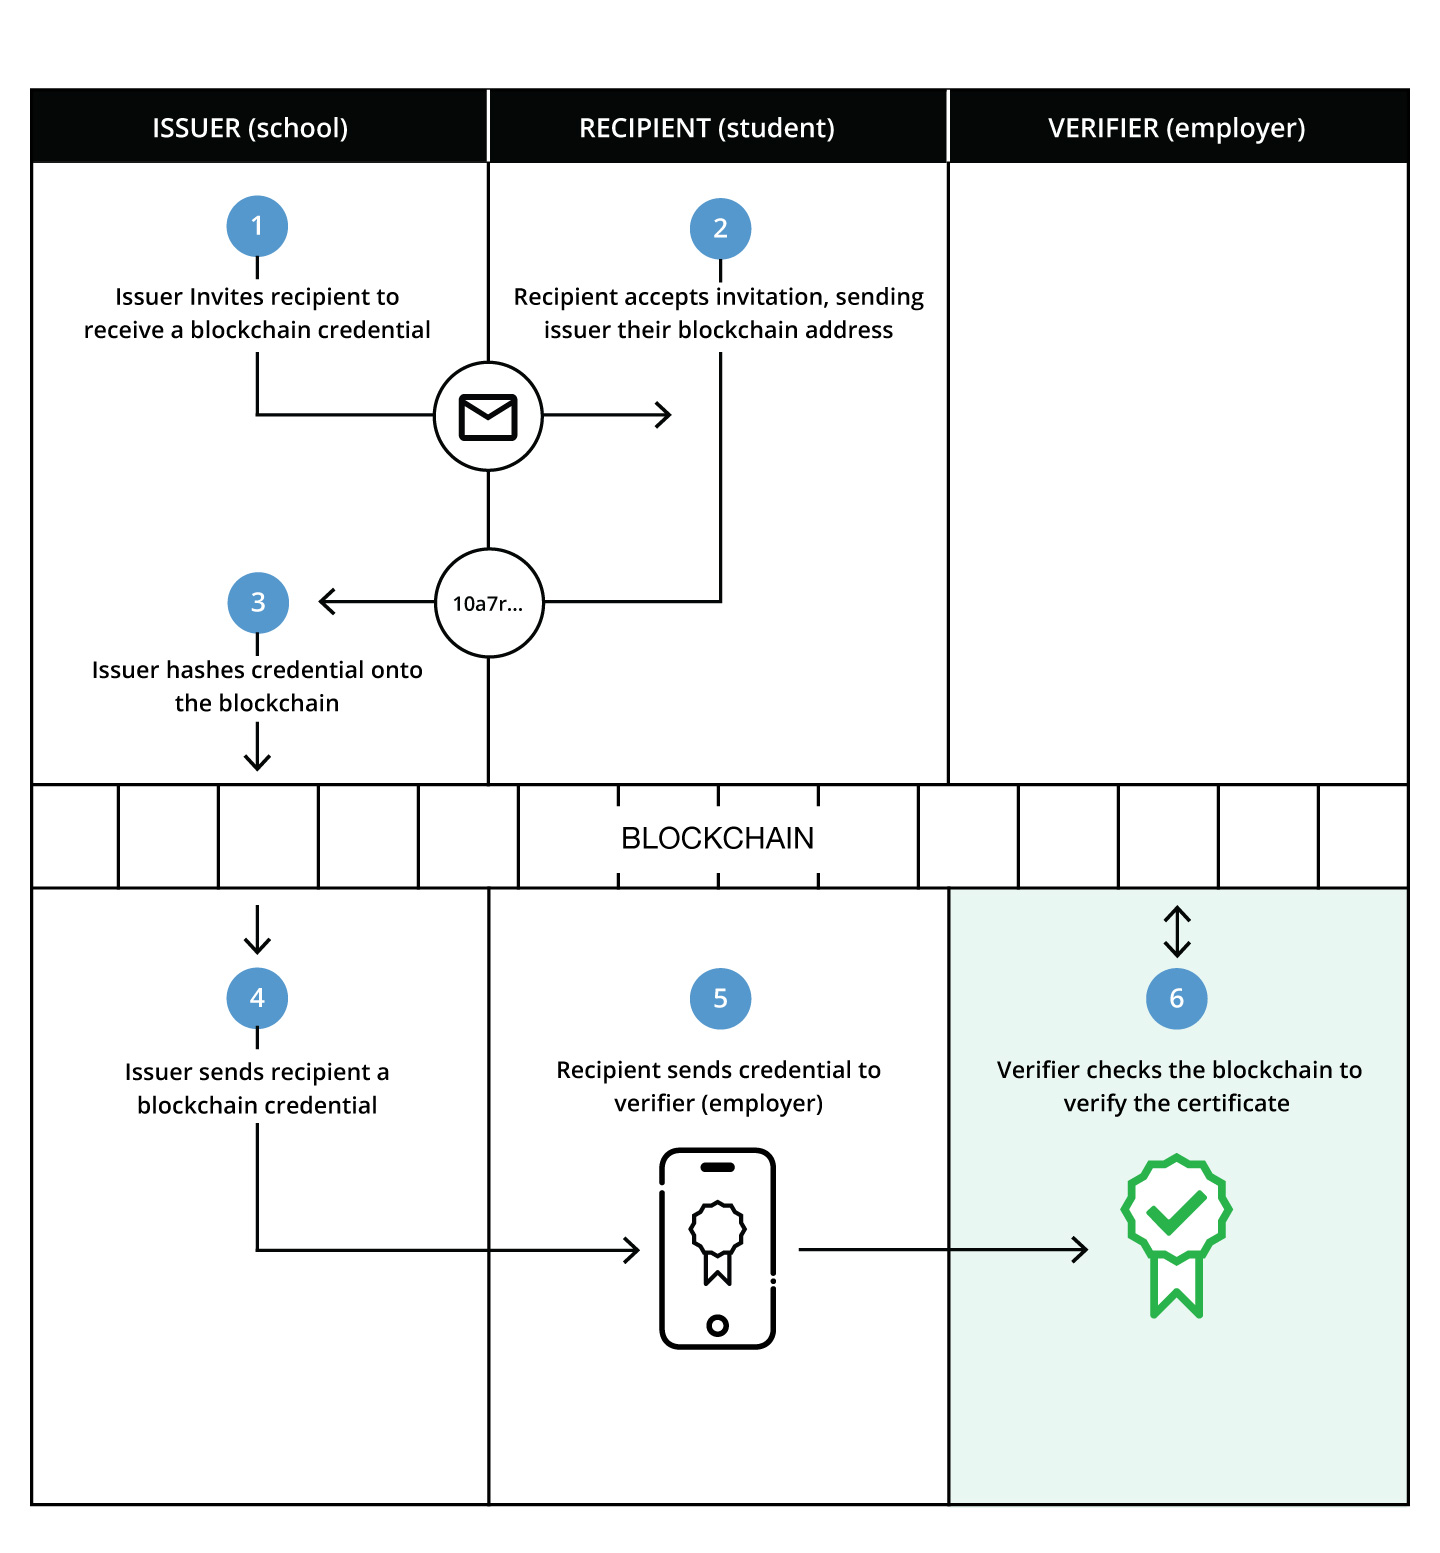
\includegraphics[scale=0.3]{blockcerts_how_it_works.jpg}}
%   \caption{Imagen extraída de la página oficial de BlockCerts}
%   \label{img:blockcerts_how_it_works}
% \end{figure}

% Este es el flujo básico que también se 
% puede visualizar en  la figura \ref{img:blockcerts_how_it_works}   para comprobar que
% un certificado se encuentra almacenado en la  Blockchain y es validado por un instituto.

% En el paso 1, el emisor o institución invita a un usuario a que brinde su dirección de cuenta o su clave pública creada 
% descargando, la aplicación movil que provee BlockCerts. En el paso 2, el usuario envía al emisor su clave pública.
% El paso 3 y 4, el emisor crea el hash a partir del certificado y lo almacena en la  Blockchain para luego enviar un archivo de tipo json \footnote{JavaScript Object Notation es un formato basado en texto estándar para representar datos estructurados \cite[]{mozilla_trabajando_json}.}, que contiene
% la información sobre el documento al estudiante o dueño del certificado. En el paso 5, puede enviar este documento a cualquier empresa o individuo que dese.
%  En el paso 6 el usuario que contiene el archivo puede verificarlo en el sitio web de  BlockCerts \cite[]{blockcerts_introduction_nodate}. 

% Este estándar es muy completo y permite a los usuarios gestionar sus propios certificados, pero lo que se busca en la investigación, 
% es desarrollar una propuesta de sistema donde un usuario puede abstraer el concepto de  Blockchain sin controlar una cuenta, enfoncadonce solamente en mantener guardados
% sus certificados.


% Otra sistema es OpenCerts que funciona generando 
% un código único a partir del certificado e información extra considerada como necesaria para validar el documento en el futuro, y luego se crea un archivo con extensión  “.opencerts ”;
% Dicho archivo se al sitio web de OpenCerts y compara el contenido con el almacenado en la  Blockchain para verificar si a existido el certificado en cuestión.
% Para dar de alta los certificados usa smart contract donde también crean los métodos para emitir o revocar un documento.

% \begin{figure}[H]
%   \centering
%   {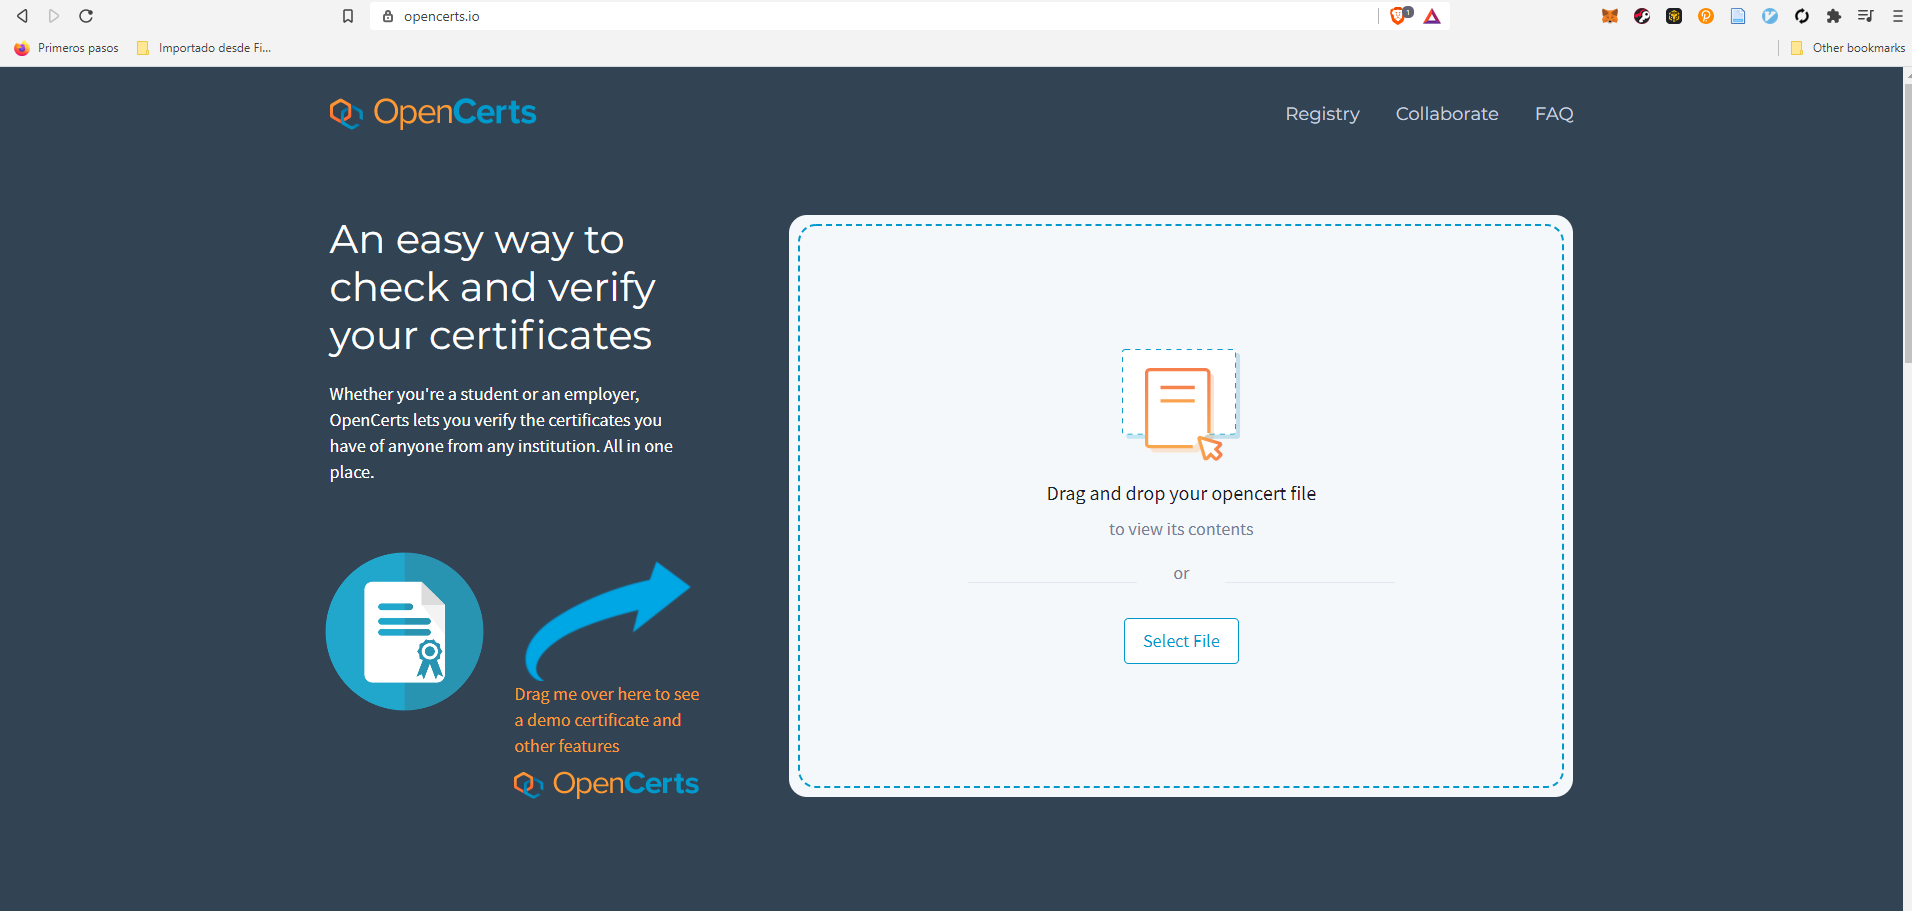
\includegraphics[scale=0.3]{OpenCerts_Home.png}}
%   \caption{página Web de OpenCerts}
%   \label{img:opencerts_home}
% \end{figure}

% En la imagen \ref{img:opencerts_home} se puede observar lo sencillo que es verificar un documento. Simplemente se arrastra el  archivo de extensión“.opencerts”
% y se buscará en la  Blockchain si realmente fue emitido por alguna entidad.
% OpenCerts utiliza los smart contract en la  Blockchain de Etherum. También utiliza tecnologías como Ract.js, Metamask, Web3.js, entre otros. Lo que permite desarrollar
% un sistema de certificados totalmente descentralizados \cite[]{opencerts_gestion_nodate}. 


 La \gls{bfa}, la cual es una  Blockchain que utiliza el protocolo de consenso llamado  prueba de autoridad. El sitio web cuenta con una herramienta llamada sello de tiempo 2.0, que permite verificar cuándo se  selló un archivo y en qué bloque,
permite confirmar que (desde esa fecha) el archivo en cuestión no sufrió modificaciones. Utiliza el mismo método que las anteriores tecnologías, 
crear un hash a partir de un archivo y almacenar el hash en la Blockchain \cite[]{Blockchain_federal_argentina_bfa_2020}.

Estas tecnologías, permiten demostrar que una secuencia de bits o cualquier tipo de archivo (puede ser
 un documento o certificado) se mantuvo inalterable a partir del día que se almacenó su hash en la Blockchain o identificador único. Algunas de ellas 
cuentan con un flujo y trabajo más elaborado, pero al fin todas cumplen con el objetivo de asegurar a los interesados si existió algún cambio en datos
del documento o archivo en cuestión. 
Luego de analizar el funcionamiento de éstas, se pretende realizar una propuesta de sistema, que permita a una institución principalmente 
a la \gls{fce} emitir sus certificados validados y los participantes de los eventos  demostrar que sus 
 documentos digitales son totalmente auténticos y correspondiente  a su persona \cite[]{opencerts_gestion_nodate,blockcerts_faq_nodate,Blockchain_federal_argentina_bfa_2020}. 

\subsection{ Análisis de Tecnologías para Desarrollar en Blockchain}

Existen diferentes tecnologías para elaborar un sistema que necesita comunicarse con una red de peer to peer y leer o escribir en la Blockchain.
Primero hay que definir cómo se almacenará la información en la Blockchain, si hacerlo en una transacción de cualquier  Blockchain (como lo hace
BlockCerts) o realizar una lógica y almacenarla en una  Blockchain que soporte contratos inteligentes.
La ventaja de los smart contract es que permiten almacenar información específica como ser el nombre de una institución, sus participantes o
cualquier dato que se desee en una sola transacción o invocación a un método del smart contract ( mientras que el primer método se necesitará 
almacenar diferentes datos en diferentes transacciones, o realizar un hash que representará que un documento sigue inalterable).



Por conveniencia de esta investigación se almacenarán datos en los smart contact, permite obtener información directamente de 
la  Blockchain, como ser el nombre, áreas, eventos de la institución. Esta diferencia da lugar a la creación de aplicaciones, por la 
conveniencia de almacenar datos que pueden ser recuperados y leídos, permitirá tener seguridad par evitar cambios no autorizados y asegurar que la información este disponible,
, en comparación con el estándar de BlockCerts que permite hacer lo mismo, pero se necesita el archivo que almacena toda la información del emisor \cite[]{opencerts_gestion_nodate,blockcerts_introduction_nodate}.
A partir de este punto se enumeran las diferentes herramientas necesarias, para el desarrollo de un sistema de validación de certificados usando Blockchain.


Lo más importante es elegir la  Blockchain que se utilizará para las pruebas y desarrollo. Existen 
las  Blockchain locales y online, también Blockchains principales y de pruebas.
Están las  Blockchain de Ethereum, Binance Smart Chain, EOS, como redes principales y online; redes de pruebas como
Ropsten, Rinkeby, entre otros.  Una de las herramientas es Ganache \footnote{\url{https://www.trufflesuite.com/ganache}}, que permite
levantar una  Blockchain  local con configuraciones personalizadas.
La diferencia entre las  Blockchain serán los algoritmos de consenso propios de la red, la cantidad de nodos, pero 
para el desarrollo de la propuesta de sistema esas característica no son necesarias, mientras que la red se comporte similar a la de una red principal, la
cual estas últimas son más seguras.
Dependerá seleccionar la  Blockchain según las necesidades de la propuesta, si se utiliza los smart contract o otra manera \cite[]{truffle_suite_ganache_nodate}.

\subsubsection{Comunicación con Blockchain}
Es necesario un método o herramienta para comunicar las transacciones que se deben realizarse 
en la Blockchain, para ello se precisa de una wallet o billetera que permita enviar las transacciones 
y comunicarse con los smart contract, en este caso existen diferentes wallet, pero una de las usadas por desarrolladores
es Metamask, permite gestionar las cuentas de los usuarios de manera local, conectarse con diferentes Blockchain, 
recibir y enviar dinero e interactuar con los Smart Contract.
Se instala como una extensión del navegador en Google Chrome o Firefox,  es usado como puente entre una aplicación y la Blockchain \cite[]{dannen_introducing_2017,metamask_introduction_2021}. 
La herramienta se puede observar en la figura \ref{img:metamask_wallet}.
\begin{figure}[H]
  \centering
  {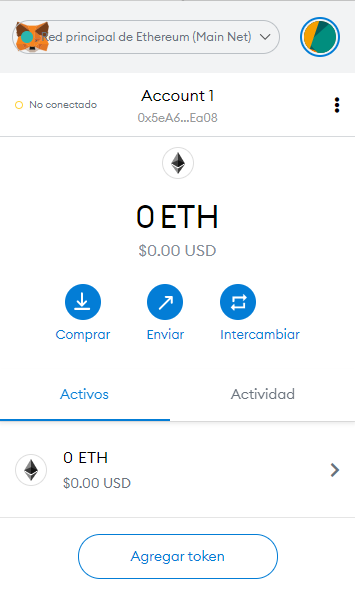
\includegraphics[scale=0.7]{MetaMask_Wallet.png}}
  \caption{MetaMask Plugin imagen extraída}
  \label{img:metamask_wallet}
\end{figure}
Por otro lado para la invocación de los métodos del contrato inteligente, se usa web3.js, que aporta las funcionalidades
necesarias para realizar las llamadas de procedimientos remotos a los nodos de la Blockchain, por la cual se pueden leer y escribir datos  abstrayendo la comunicación directamente 
y la creación de las transacciones, mientras la gestión de la cuenta de lo usuarios se realiza con MetaMask \cite[]{dannen_introducing_2017}.



\subsubsection{Programación en Blockchain}

Se deberá  decidir en qué  Blockchain se trabajará, porque los smart contract se escriben en un lenguaje específico,
en el caso de Etherum es Solidity, pero existen un gran número de  Blockchain que utilizan la misma estructura de Etherum para generar 
su propia  Blockchain con algunas diferencias, pero en cuanto al lenguaje de programación  para el desarrollo de los smart contract 
es el mismo. En este caso se utilizará Solidity porque existen documentaciones que describen su uso y es la más usada para el desarrollo de smart contract \cite[]{dannen_introducing_2017,ethereum_solidity_nodate}

\subsubsection{Publicación de Smart Contract}
Es necesario utilizar una herramienta  que permita enviar el código escrito con el lenguaje Solidity a la Blockchain, para 
ello existen herramientas tales como Remix o Truffle, las que permiten compilar y almacenar el smart contract en una red de prueba local como online.
En el caso de Remix es una herramienta que puede usarse de manera online o local. Permite desplegar el código en una  Blockchain de prueba local o 
de prueba online como Ropsten o una Mainnet como Etherum \cite[]{remix_deploy_nodate}.
 Truffle es un entorno de desarrollo, marco de pruebas y canalizados de activos para cadenas de bloques que utilizan la máquina virtual Ethereum (EVM), con el objetivo de facilitar el desarrollo
de proyectos con Blockchain, permite desplegar también de manera pública o privada, así mismo provee otras facilidades como gestión de paquetes,
automatización de pruebas, entre otras \cite[]{truffle_truffle_nodate}. 






\subsubsection{Desarrollo del font-end}
Se deben seleccionar las  herramientas que se necesitan para la creación de la interfaz de los usuarios 
que pretenden gestionar la información relacionada a la documentación digital y a la institución.
Al utilizar las tecnologías mencionadas, es necesario  un desarrollo web, donde se puede obtener  un servidor central o descentralizado
para almacenar datos de usuario, y conectando 
el front-end con la  Blockchain directamente. Esta última es conveniente para evitar manejar datos sensibles 
porque serían visibles a todo público, puede verificar la existencia de los datos y 
el servidor central no es necesario para la validación de documentos.
Para el desarrollo de un front-end es necesario la utilización de  tecnologías como  HTML, javascript y CSS o utilizar un framework como
ReactJS, VueJS o AngularJS, para desarrollar el sistema de manera organizada incluyendo todo lo requerido para la interfaz de usuario \cite[]{dannen_introducing_2017,educacionit_carrera_nodate}.

Para la creación de un sistema de validación de documentos digitales es conveniente utilizar los puntos importantes   del estándar BlockCert y  la utilización de los smart contract 
como lo hace OpenCert, también existen códigos fuentes que pueden ser reutilizados. Uno de ellos
son las herramientas que provee la  \gls{bfa}, por ejemplo la interfaz para que un usuario valide o selle un documento, este
código se encuentra escrito en VueJS, por lo que se optará
su uso para el desarrollo de la vista del usuario. Cabe aclarar que se puede realizar con cualquier otro framework (esto se puede
demostrar encontrando los diferentes proyectos existentes con diferentes tecnologías usadas o en cursos de desarrollo de  Blockchain con ReactJS 
% \footnote{\href{https://codeburst.io/build-a-cryptocurrency-dashboard-with-react-d9e476de91ef?gi=854fd33c74d7}{Ejemplo par Desarrolar con React}}.
o AngularJs \cite[]{Blockchain_federal_argentina_bfa_2020}. 
% \footnote{\href{https://medium.com/Blockchain-developer/learn-how-to-create-your-own-dapp-with-angular-part-i-688f24e0ad9e}{Ejemplo de como Desarrollar con Angular.}}).

\subsubsection{Criptografía}
La función hash es necesaria como parte de cualquier proyecto de documentos digitales visto, como lo usan BlockCert y OpenCert, también
las propias  Blockchain la usan para crear las direcciones de los bloques. Asimismo la \gls{bfa} usa esta función hash. 
Existen diferentes tipos como MD5, SHA y sus variaciones  por lo general en las Blockchains y 
en los sistemas o aplicaciones utilizan SHA-256, por su uso extendido  se elije esta última \cite[]{satoh_asic-hardware-focused_2007}.



\section{Análisis de la Propuesta de Sistema de Validación de Documentos Digitales}

Para que el sistema permita validar documentos digitales sin almacenar la información contenida en ella y 
evitar acceder a datos sensibles de un individuo, se utilizarán los métodos de los estándares o sistemas (BlockCerts y OpenCerts). En otras palabras, genera
un hash a partir de una secuencias de caracteres como valores de entrada y  se obtiene una salida de longitud fija, de este modo se  aumenta la dificultad
para conocer el contenido del documento y se genera un identificador único, el hash asegura que el documento no fue modificado y puede ser verificado usando nuevamente 
el mismo archivo original \cite[]{blockcerts_introduction_nodate,jirgensons_Blockchain_2018}.
Luego se necesitará información adicional, como ser el día en el cual el documento se creó, o si esta relacionado a algún evento de la organización que la emitió,
nombre de la organización, el nombre del Área o Departamento encargado de generar el documento y los datos extras que se necesiten. Por otro lado 
permitir a los encargados de emitir los certificados poder cambiar los estados de los documentos, por ejemplo, si pasado un tiempo un documento
ya no tiene validez, se puede cambiar el estado del documento a no válido, o darle una fecha de expiración si se necesitara.
Con esta información se creará   un smart contract que permita almacenar estos datos en la Blockchain, manteniéndolos inmutable 
a menos que se permita roles a usuarios específicos, con permisos para modificarlos.

\subsection{Bases del Sistema}\label{ss:basesistema}
La base del sistema es  mantener los documentos digitales o el hashes inalterables, para asegurar
que el contenido no cambió.

En primer lugar es gestionar los tipos de documentos que se manejan, definir cómo se almacenarán y asignarán  el/los
responsable/s de hacerlo, con la  posibilidad de cambiar algunas características de los documentos digitales \cite[]{opencerts_gestion_nodate}.
Por ejemplo, manejar estados de los documentos, que permita a los interesados de validar si el documento
fue emitido por la universidad o una institución. Los estados sirven para 
que el interesado pueda observar si la documentación venció o si está en algún estado específico.   
Los datos usados por los estándares como BlockCert y OpenCert son el hash del documento, que una vez almacenado
no se permite cambiarlo, cambiar estados, definir una fecha de creación y una fecha de expiración.

Los estándares  almacenan información relacionada con el lugar donde se emitió el documento \cite[]{opencerts_gestion_nodate}, esto se logra 
agregando información como el evento  que lanzó el certificado, por ejemplo, un cursado, un examen, etc, cualquier situación que pueda 
generar una documentación digital \cite[]{mit_media_lab_what_2016}.
El evento puede suceder en un lapso de tiempo o puede ser indeterminado, por ejemplo, 
un evento de un curso que su duración son 3 días, o un evento que inicia una fecha pero no se conoce cuando finalizará.

Los eventos suceden en algún sitio o área, al observar  la \glsfirst{fce} de la \glsfirst{unam} 
la Secretaría de Extensión es la encargada de realizar los eventos o actividades como cursos, o 
actividades externas, por ende, el  área encargada es la Secretaría de Extensión (A.L., comunicación personal, 02/10/2020).%\cite[]{larraburu_secretariextension_2020}.

Se podrá almacenar información como el nombre y las áreas de la institución, con  estos datos se obtiene qué área almacenó el documento digital, conocer el evento que 
se generó en una fecha determinada o indeterminada, si el documento puede caducar, y por último, 
si el documento fue generado por la institución, dando una validez de que existe en la Blockchain.

Estas informaciones, se obtuvieron de   relevamientos que explican  el funcionamiento de las aplicaciones para certificados digitales y las informaciones que son usadas
frecuentemente. Por  ejemplo, el estándar BlockCerts que almacena el hash del documento e información relacionada
al emisor \cite[]{blockcerts_faq_nodate}.

% \subsection{Diseño de la lógica}
% A continuación se muestra un diagrama de flujo de datos.

% \begin{figure}[hbt!]
%   \centering
%   {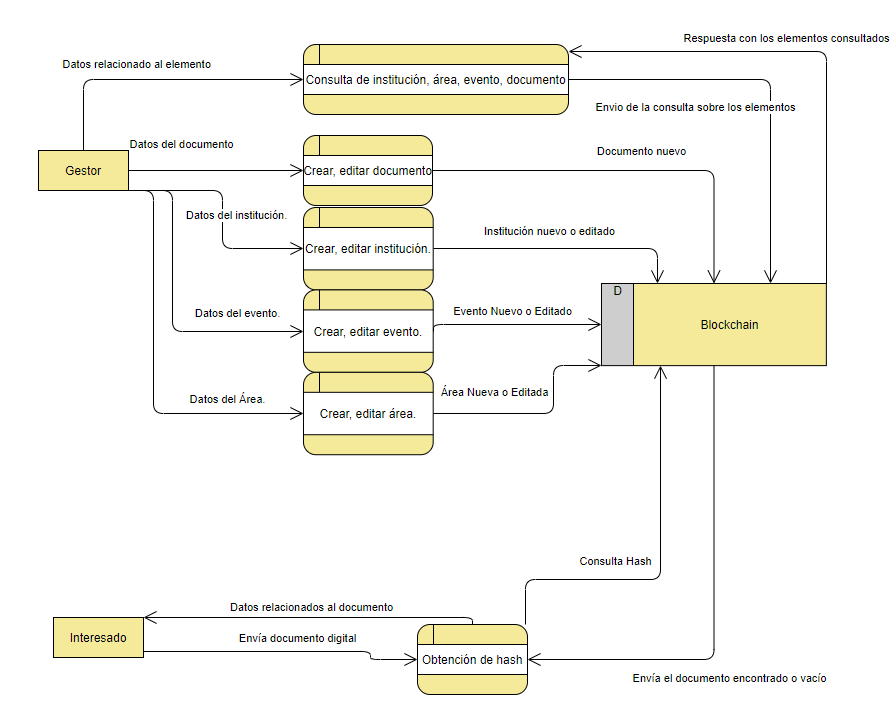
\includegraphics[scale=0.7]{Diagrama_Validacion_Documento.png}}
%   \caption{Diagrama de Flujos de datos, elaboración del Autor}
%   \label{img:flujo-datos}
% \end{figure}

% En la figura \ref{img:flujo-datos} se puede observar cómo fluyen los datos, el diagrama es una solución genérica sin entrar a los detalles.
% Pero el flujo de los datos serían principalmente almacenar los datos relacionados a un documento digital especifico. A partir de 
% uno o algunos responsables, ya que si cualquier individuo puede almacenar esta información, no tendría ninguna validez,
% por lo tanto solo los documentos almacenados mediante el uso del smart contract  serán válidos.

% Los interesados en el diagrama representan a cualquier individuo (como el propio dueño del documento digital, o una autoridad de la organización o persona externa de ella)
%, pudiendo obtener datos relacionado con el documento quién fue el emisor o si el documento fue realmente subido por la organización. 
% Pero para poder realizar tal verificación debe tener el documento digital en su posesión; de esta forma comprobar si 
% el contenido del documento no fue modificado y que fue emitido por la organización.

% Los gestores son los encargados de almacenar la información y serían personas que recae la responsabilidad
% de los documentos que se emiten.

\subsection{Solución Propuesta}
Para validar los documentos digitales de la Secretaría de Extensión de la \gls{fce} de la \gls{unam}, se propone crear un sistema,
basado en los protocolos definidos para la validación de documentos se utilizada tecnología Blockchain, 
para ello se realizará un smart contract que tendrá la lógica necesaria para almacenar datos relacionados
al documento, sin exponer datos sensibles de los intervinientes, y permite la validación del documento que permaneció sin cambios. 
También gestionar información de los documentos y cambiar estados futuros de ellos, almacenar 
el documento en la  Blockchain permite crear una relación única entre una cuenta y la información guardada,
habilita  seguir consultando los datos en el futuro. 

















 












%---------------- Elaboración de solución ------------------------
%% Diseñar un modelo teorico enfocnadome en todas las referencias bibliograficas

%% -------------- Desarrollo de la solución -----------------------------------
% Realizar el proceso de como se construye el sistema propuesto para la certificaciones.
\chapter{Desarrollo del Sistema Propuesto}
En este capítulo se desarrolla la solución al problema de la falta de validacion de documentos digitales emitidos por la Secretaría 
de Extensión de la \gls{fce} de la \gls{unam}.
Se realiza el diseño teórico que se pretende aplicar y se define su funcionamiento y las relaciones entre las
herramientas y tecnologías en la implementación. 

\section{Tecnologías y Herramientas Seleccionadas}
Las tecnologías y herramientas seleccionadas para el desarrollo de la propuesta son:
\begin{enumerate}
    \item La red de prueba llamada Ropsten, esta  Blockchain de prueba  permite publicar los smart contract
    y la emisión de su token de prueba es de forma gratuita, cuenta con pocos nodos pero el objetivo 
    de su uso es hacer pruebas en esta red, su comportamiento es similar a otra  Blockchain con maquina virtual de Ethereum \cite[]{dannen_introducing_2017}.
    \item Solidity como lenguaje de programación para los contratos inteligentes \cite[]{dannen_introducing_2017,bragagnolo_smartinspect_2018}.
    \item Node JS con su gestor de paquetes para instalar las librerías necesarias.
    \item Web3.js una librería de javascript que permite conectarse a la  Blockchain de una manera más rápida y abstrayendo la complejidad de la comunicación
    con la Blockchain \cite[]{dannen_introducing_2017}.
    \item SHA-256 un algoritmo de hash, pero también existen diferentes  librerías de  javascript que permite generar un hash a partir de caracteres.
    \item Vue.js un framework de javascript, para facilitar el desarrollo del front-end, reutilizando partes de otros proyectos open sources.\cite[]{vuejs_introduction_nodate}
    \item Para la publicación de los contratos inteligente se usará Remix, es una de las tecnologías ya mencionadas y su uso 
    es intuitivo \cite[]{remix_deploy_nodate}.

\end{enumerate}

Estas tecnologías permitirán crear el sistema para validar los documentos de la Secretaría de Extensión de la \gls{fce} de la \gls{unam}, dando el beneficio 
a terceros de verificar que el contenido de un documento  es correcto y no fue alterado \cite[]{brys_cadena_2019}. 

\section{Diseño de la Lógica}
A continuación se muestra un diagrama para comprender los datos  esenciales para el diseño del sistema.

\begin{figure}[H]
  \centering
  {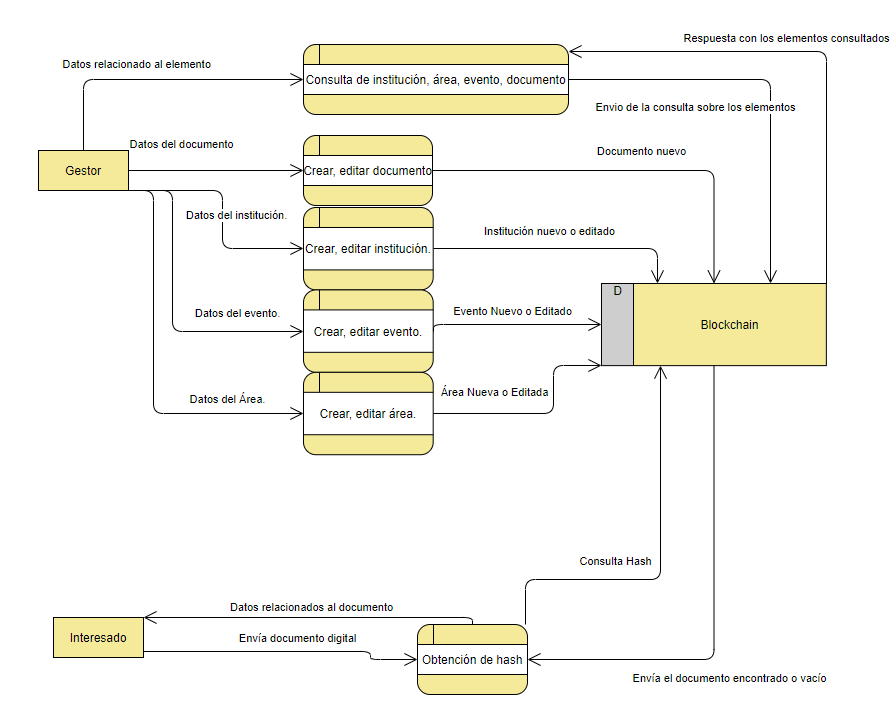
\includegraphics[scale=0.6]{Diagrama_Validacion_Documento.png}}
  \caption{Diagrama de Flujos de datos, Fuente: producción propia.}
  \label{img:flujo-datos}
\end{figure}

En la figura \ref{img:flujo-datos} se observa el flujo de los datos que se manejan en una validación de certificados, principalmente se almacenan los datos en la Blockchain y son leidos por las personas interesadas. Los responsables 
de sus áreas deben  almacenar los datos en la Blockchain, esto permitirá validar que los documentos almacenadas solamente
serán cargados por personal autorizado.    

% El flujo de los datos de la figura \ref{img:flujo-datos} será principalmente almacenar los datos relacionados a un documento digital específico. Por parte de 
% uno o algunos responsables, ya que si cualquier individuo puede almacenar esta información, no tendría ninguna validez,
% por lo tanto solo los documentos almacenados mediante el uso del smart contract  serán válidos.

Los interesados en el diagrama representan a cualquier individuo (como el propio dueño del documento digital, o una autoridad de la organización o persona externa de ella), 
se puede obtener datos relacionados con el documento quién fue el emisor o si el documento fue realmente subido por la organización. 
Pero para poder realizar tal verificación debe tener el documento digital en su posesión; de esta forma comprobar si 
el contenido del documento no fue modificado y que fue emitido por la organización.

Los gestores son los encargados de almacenar la información y serían las personas responsables 
de los documentos emitidos.

\section{Diseño de Sistema}\label{s:system_design}

En la sección \ref{ss:basesistema}  se explica de manera genérica, los datos necesarios 
para validar un documento digital en base a los estándares BlockCert y OpenCert.
Para ello se diseña un diagrama de la figura \ref{img:diagrama_clases} para la propuesta del sistema para validación de documentos:  

\begin{figure}[H]
    \centering
    {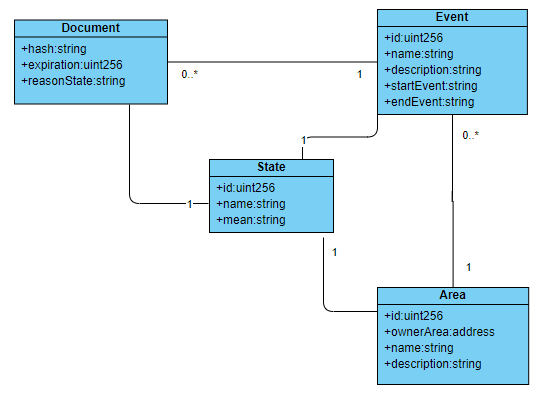
\includegraphics[scale=0.7]{diagrama_clases.png}}
    \caption{Diagrama de domino, Fuente: producción propia.}
    \label{img:diagrama_clases}
  \end{figure}

  En la figura \ref{img:diagrama_clases} se puede observar la propuesta de  construcción del sistema basándose 
  en el estándar de BlockCerts donde se almacenan los hashes del documento e información relacionada a ella \cite[]{blockcerts_introduction_nodate,criptomonedas_tv_entrevista_2018,blockcerts_faq_nodate}, 
  el diagrama muestra un área que es la responsable 
  de emitir los certificados, sin revelar datos de personas o contenido del documento. Por lo tanto el objetivo
  de no incluir  datos sensibles quedan cubiertos. 

  Se analizaron los requerimientos de la universidad y en conjunto a la entrevista (A.L., comunicación personal, 02/10/2020) para poder diseñar la lógica del sistema. Se incluyeron administradores o los propietarios (owner) 
  de las áreas, serían los responsables de almacenar los hashes de  documentos que se generen en los Eventos de las Áreas,
  cuando se habla de los eventos, se los trata como  genéricos, un evento puede ser una clase, una charla, un congreso o inclusive
  una determinada hora del día, de esta manera los documentos pueden estar relacionados a los eventos que ocurren.

  La construcción, el almacenamiento  y lectura  de datos de una aplicación  en la  Blockchain es diferente a una 
  aplicación centralizada, por ejemplo, los datos almacenados no se consultan mediante lenguaje SQL, tampoco se puede agregar nuevas
  variables una vez almacenado en la Blockchain, en cambio en una base de datos centralizada si se pueden agregar nuevos atributos \cite[]{dannen_introducing_2017,mayor_Blockchain_2017}.

 En resumen el dominio comprende áreas, eventos, estados y los documentos cada uno de ellos
 almacena datos representativos y básicos para validar la existencia de un documento digital en la Blockchain. 

  \subsection{Estructura del Smart Contract}
  Definir  los datos necesarios para la propuesta del sistema, permite dar forma a 
  la estructura del smart contract, ya que éste no cambiará una vez que sea publicado en la Blockchain, pero no significa
  que se pueda publicar otras versiones. La propuesta es utilizar una  Blockchain de prueba  para realizar todos los intentos necesarios 
  hasta obtener el funcionamiento del sistema. 

  La estructura del smart contract será como se refleja en la figura \ref{img:smart_contract_structure}, a continuación se explican cada parte de ella:

  
\begin{figure}[hbt!]
    \centering
    {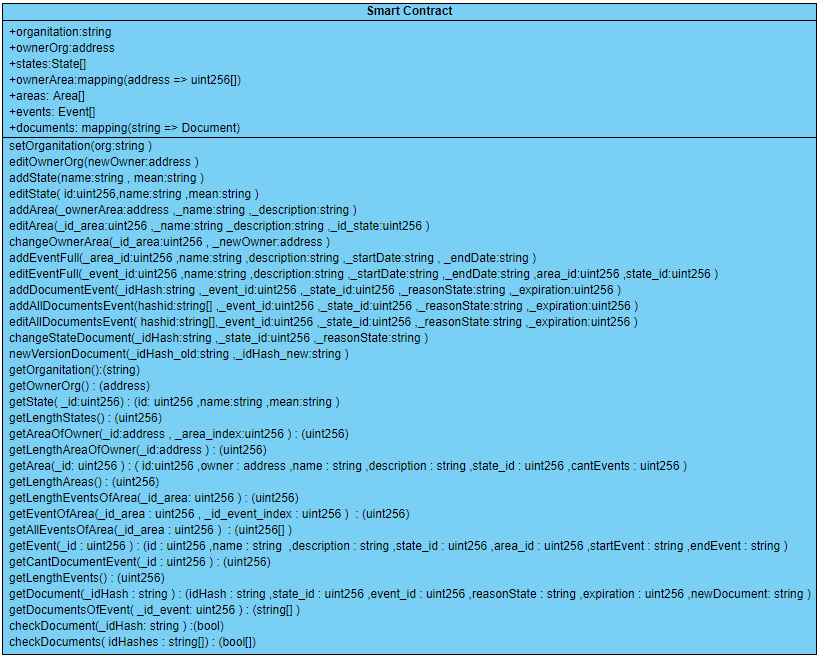
\includegraphics[scale=0.5]{smart_contract_abstract.png}}
    \caption{Smart Contract estructura, Fuente: producción propia.}
    \label{img:smart_contract_structure}
  \end{figure}
Los atributos (de la figura \ref{img:smart_contract_structure} ) que almacenarán los datos necesarios serán los siguientes :
  \begin{itemize}
    \item \textit{\textbf{ organitation: string}}, se almacenará el nombre de la organización responsable de las áreas, eventos y todos los documento digitales.
    \item \textit{\textbf{ownerOrg: address}}, la dirección de la cuenta del único responsable para manejar todos los datos del smart contract.
    \item \textit{\textbf{states: State[]}}, los posibles estados que maneja el sistema, como ser estado revocado, el cual el estándar BlockCert y OpenCert lo usan \cite[]{blockcerts_faq_nodate,opencerts_gestion_nodate}.
    \item \textit{\textbf{ownerArea:mapping(address => uint256[])}}, son el conjunto de direcciones que están encargadas de manejar una o varias áreas especificas. Estos owner deberían ser agregados por el owner de la organización para evitar que un individuo desconocido tenga el poder de modificar datos.
    \item \textit{\textbf{areas: Area[]}}, el conjunto de áreas de la organización.
    \item \textit{\textbf{events: Event[]}}, los eventos que pueden surgir en un área especifica y encargados de generar los documentos digitales.
    \item \textit{\textbf{documents: mapping(string => Document)}}, los hashes de documentos asociado a la información del documento.
    \end{itemize}

    La notación que se utilizó para el diagrama \ref{img:smart_contract_structure} para los tipos de datos son de la misma manera
    en la que se definen en Solidity,
    como por ejemplo la definición de mapping(string => Document). Esto sirve para definir  una variable  que recibe como
    índice un string por ejemplo “A”  referencia un documento almacenado en la Blockchain. El string se creó como índice para 
    que el usuario pueda usar cualquier tipo de algoritmo de hash y el sistema permita almacenar en la  Blockchain sin tomar en cuenta la función hash
   , esta idea es usada por los estándares ya mencionados \cite[]{opencerts_gestion_nodate,blockcerts_introduction_nodate,blockcerts_faq_nodate}. 

    Los métodos para realizar cambios en los datos del sistema:
    \begin{itemize}
      \item \textit{\textbf{setOrganitation(org:string)}}, el método permite cambiar el nombre de la organización, sólo debe ser ejecutado por el propietario de la organización.
      \item \textit{\textbf{editOwnerOrg(newOwner:address)}}, permite cambiar al único usuario que podrá ejecutar todos los métodos.
      \item \textit{\textbf{addState(name:string, mean:string)}}, name es el nombre del estado y mean el significado o para qué se usaría. El método agrega un nuevo estado que podrá ser usado por las áreas, eventos y documentos.
      \item \textit{\textbf{editState( id:uint256, name:string, mean:string)}}, edita el nombre y el significado del estado.
      \item \textit{\textbf{addArea(ownerArea:address, name:string, description:string)}}, crea un nuevo estado y pasa por parámetros la dirección del dueño o responsable del área a crear, el nombre, y una descripción como dato extra. El único que puede ejecutar este método es la dirección que concuerde con la ownerOrg
      \item \textit{\textbf{editArea(id\_area:uint256, name:string description:string, id\_state:uint256)}}, el id que representa el área a editar, los datos a modificar como el nombre, la descripción y el estado actual.
      \item \textit{\textbf{changeOwnerArea(id\_area:uint256, newOwner:address)}}, permite cambiar el propietario de un área específica.
      \item \textit{\textbf{addEventFull(area\_id:uint256, name:string, description:string, startDate:string, endDate:string)}}, agrega un evento a la  Blockchain relacionándolo, con un área especifica.
      \item \textit{\textbf{editEventFull(event\_id:uint256, name:string, description:string, startDate:string, endDate:string, area\_id:uint256, state\_id:uint256)}}, edita la mayoría de los atributos de un evento.
      \item \textit{\textbf{addDocumentEvent(idHash:string, event\_id:uint256, state\_id:uint256, reasonState:string, expiration:uint256)}}, crea un documento nuevo con relación a un evento particular y una fecha de vencimiento para el documento digital. La fecha
      es representada por un valor numérico o \gls{TimeStamp}.
      \item \textit{\textbf{addAllDocumentsEvent(hashid:string[], event\_id:uint256, state\_id:uint256, reasonState:string, expiration:uint256)}}, permite almacenar muchos documentos enviando un array de hashes y 
      los atributos iguales que tendrán los documentos, por ejemplo todos los documentos serán del mismo evento, tendrán el mismo estado  y fecha de vencimiento.
      \item \textit{\textbf{editAllDocumentsEvent(hashid:string[], event\_id:uint256, state\_id:uint256, reasonState:string, expiration:uint256)}}, edita todos los documentos que se encuentran en el array de hashes.
      \item \textit{\textbf{changeStateDocument(idHash:string, state\_id:uint256, reasonState:string)}}, cambia el estado de un solo documento.
      \item \textit{\textbf{newVersionDocument(idHash\_old:string, idHash\_new:string)}}, se le asigna una nueva versión a un documento antiguo, idHash\_old es el documento antiguo o idHash\_new es el hash del nuevo documento,
      esto sirve para mantener versiones de un solo documento. 
    \end{itemize}

    Y por último, los métodos para lectura de los datos son:

    \begin{itemize}
      \item \textit{\textbf{getOrganitation():(string)}}, retorna un string que es el nombre de la organización.
      \item \textit{\textbf{getOwnerOrg() : (address)}}, devuelve la dirección del dueño o propietario, el cual podrá ejecutar todos los métodos.
      \item \textit{\textbf{getState( id:uint256) : (id: uint256, name:string, mean:string )}}, retorno los atributos del estado que tenga el id pasado por un parámetro.
      \item \textit{\textbf{getLengthStates() : (uint256)}}, obtiene la cantidad de estados almacenados.
      \item \textit{\textbf{getAreaOfOwner(id:address, area\_index:uint256 ) : (uint256)}}, obtiene el id de un área de un propietario de área.
      \item \textit{\textbf{getLengthAreaOfOwner(id:address ) : (uint256)}}, obtiene la longitud o la cantidad de areas de un propietario de área.
      \item \textit{\textbf{getArea(id: uint256 ) : ( id:uint256,owner : address,name : string,description : string,state\_id : uint256,cantEvents : uint256 )}}, obtiene un área a partir de un id.
      \item \textit{\textbf{getLengthAreas() : (uint256)}}, obtiene la cantidad de áreas que hay almacenado en la Blockchain.
      \item \textit{\textbf{getLengthEventsOfArea(id\_area: uint256) : (uint256)}}, la cantidad de eventos que están relacionado a un área.
      \item \textit{\textbf{getEventOfArea(id\_area : uint256, id\_event\_index : uint256)  : (uint256)}}, obtiene el id un evento relacionado a un área.
      \item \textit{\textbf{getAllEventsOfArea(id\_area : uint256 )  : (uint256[])}}, trae todos los id de eventos de un área.
      \item \textit{\textbf{getEvent(id : uint256) : (id : uint256,name : string ,description : string,state\_id : uint256,area\_id : uint256,startEvent : string,endEvent : string )}}, obtiene los atributos de un evento.
      \item \textit{\textbf{getCantDocumentEvent(id: uint256) : (uint256)}},   la cantidad de documentos relacionado a un evento.
      \item \textit{\textbf{getLengthEvents() : (uint256)}}, cantidad de eventos que existen almacenados.
      \item \textit{\textbf{getDocument(idHash : string) : (idHash : string,state\_id : uint256,event\_id : uint256,reasonState : string,expiration : uint256,newDocument: string )}}, obtiene todo los atributos de un documento a partir de su hash.
      \item \textit{\textbf{getDocumentsOfEvent(id\_event: uint256) : (string[])}}, obtiene todos los hashes de los documentos relacionado a un evento.
      \item \textit{\textbf{checkDocument(idHash: string) :(bool)}}, devuelve true si el hash del documento esta almcenado en la Blockchain.
      \item \textit{\textbf{checkDocuments(idHashes : string[]) : (bool[])}}, a partir de un array de hashes de documentos devuelve en el mismo orden true o false dependiendo si existe o no en la Blockchain
      respectivamente.
    \end{itemize}

    \subsection{Roles y Permisos}
    En la propuesta de sistema se utiliza un smart contract para el código almacenado en la Blockchain. Para ello también es necesario definir los responsables de gestionar los datos.
    Se establecen dos niveles, el primero es un usuario que pueda gestionar todo los datos, como un administrador. 
    Por ende, se debe definir el rol de un usuario o propietario del smart contract, que sea el único que tenga el poder de crear nuevas áreas,
    cambiar en nombre a la organización, editar los datos de las áreas, agregar o quitar responsables de cada área. 
    El otro nivel son los usuarios encargados de una o muchas  áreas, los cuales tienen la responsabilidad de gestionar los documentos y eventos de un área especifica,
    para ello el administrador o el propietario del smart contract decide quiénes son los operarios o encargados de crear los documentos digitales y almacenarlos en la  Blockchain mediante
    su hash.
    Esto es importante para evitar que usuarios externos a la organización controlen los documentos emitidos por la entidad. Para ello se crean los roles o niveles de seguridad.
    También habrá un usuario que no tiene el poder de modificar los datos almacenados, simplemente podrá consultar 
    acerca de los documentos y validaciones, es el individuo que requiere conocer la validez del documento y comprobar que es emitido por la organización. 
    En resumen se definen dos niveles: nivel de administrador es el encargado y responsable de todo los datos almacenados, por otro lado un nivel de encargados de  áreas.
  \subsubsection{Estructura de permisos}
  Todos los usuarios tendrán acceso a leer sus datos, por eso desde el inicio   se evita almacenar datos sensibles relacionados
  a los dueños de los documentos, mientras que los datos de la organización son públicos y pueden ser almacenados. 
  En esta sección se definirán qué comportamiento tendrán los roles y qué permisos según los niveles de usuarios. Al analizar los datos sobre los métodos y las necesidades 
  a satisfacer, se parte de tres niveles: 
  \begin{enumerate}
    \item Nivel público: el usuario podrá consultar datos almacenados, (cómo verificar si un documento existe en la Blockchain).
    \item Nivel de propietario de área: son los encargados de almacenar y crear los eventos relacionado a sus áreas, también de gestionar los documentos digitales, cambiando sus estados,
    agregando nuevas versiones.
    \item Nivel de propietario del smart contract: es la única dirección que tiene permiso de ejecutar todos los métodos. Puede cambiar el nombre de la organización,
    asignar nuevos propietarios de áreas, crear áreas, y hacer lo mismo que los demás niveles. 
  \end{enumerate}
  


\section{Desarrollo del Smart Contract}
A continuación se detallan las herramientas y las manera de utilizarlas para el desarrollo 
del Smart Contract.

\subsection{Instalación de Metamask}

Como primer paso, hay que instalar el plugin de Metamask de la  página web oficial   el navegador que se usará de prueba (en este proceso, es  Google Chrome) 
tal como se muestra en la  figura \ref{img:metamask_install}.
\begin{figure}[H]
  \centering
  {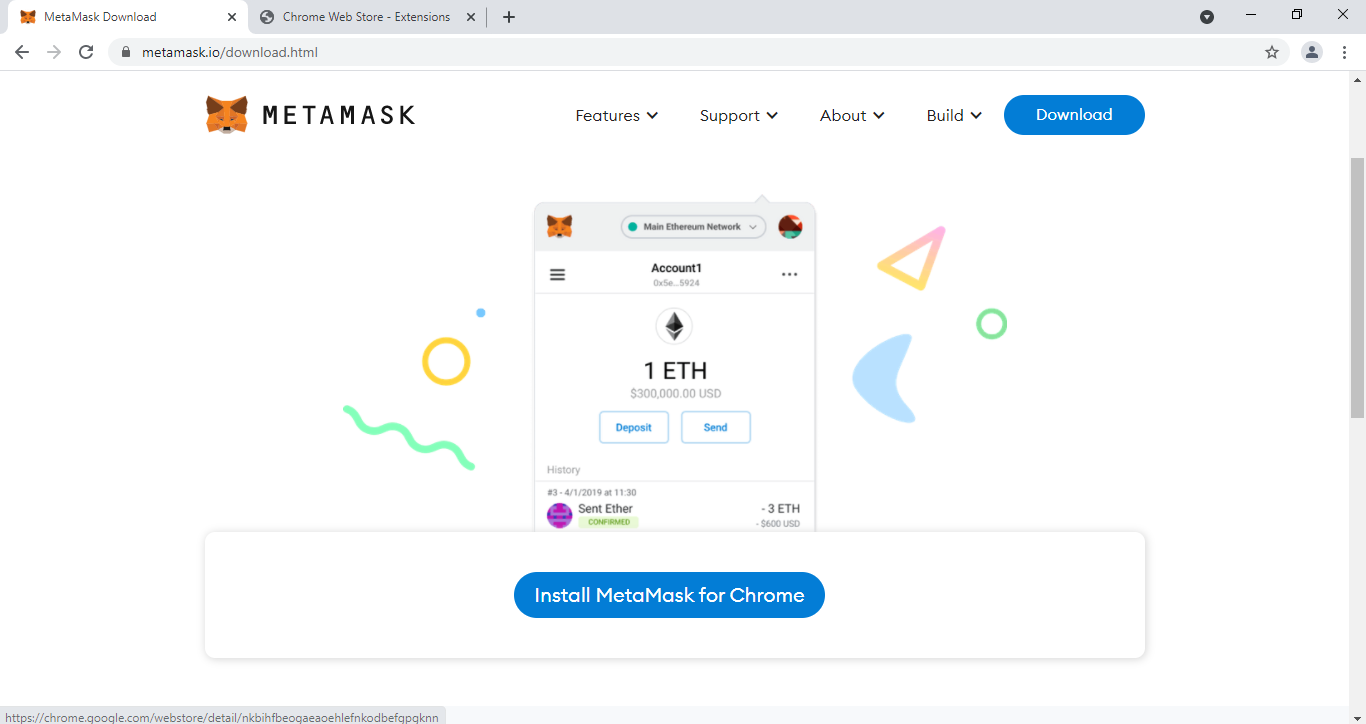
\includegraphics[scale=0.4]{metamask_install.png}}
  \caption{Página para descargar Metamask, Fuente: captura de pantalla.}
  \label{img:metamask_install}
\end{figure}

Se agrega el plugin al navegador como se ve en la figura \ref{img:metamask_add}, luego
se abrirá una nueva pestaña o en caso que no aparezca deberá buscar Metamask en sus extensiones del navegador 
para hacer clic donde este le redirigirá a una nueva pestaña para crear o importar su wallet.
Los pasos son hacer clic en Get Stated visto en la figura \ref{img:metamask_getstarted}.



\begin{figure}[H]
  \centering
  {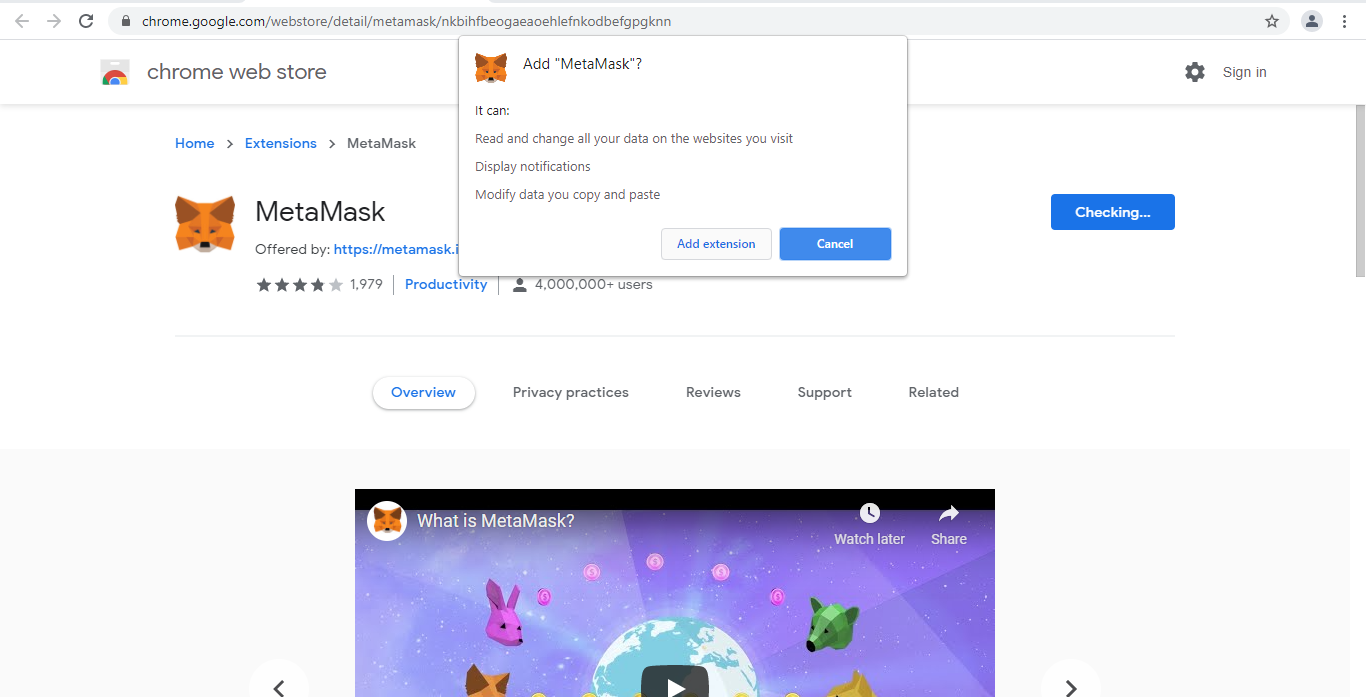
\includegraphics[scale=0.4]{metamask_addplugin.png}}
  \caption{Agregando el plugin, Fuente: captura de pantalla. }
  \label{img:metamask_add}
\end{figure}

\begin{figure}[H]
  \centering
  {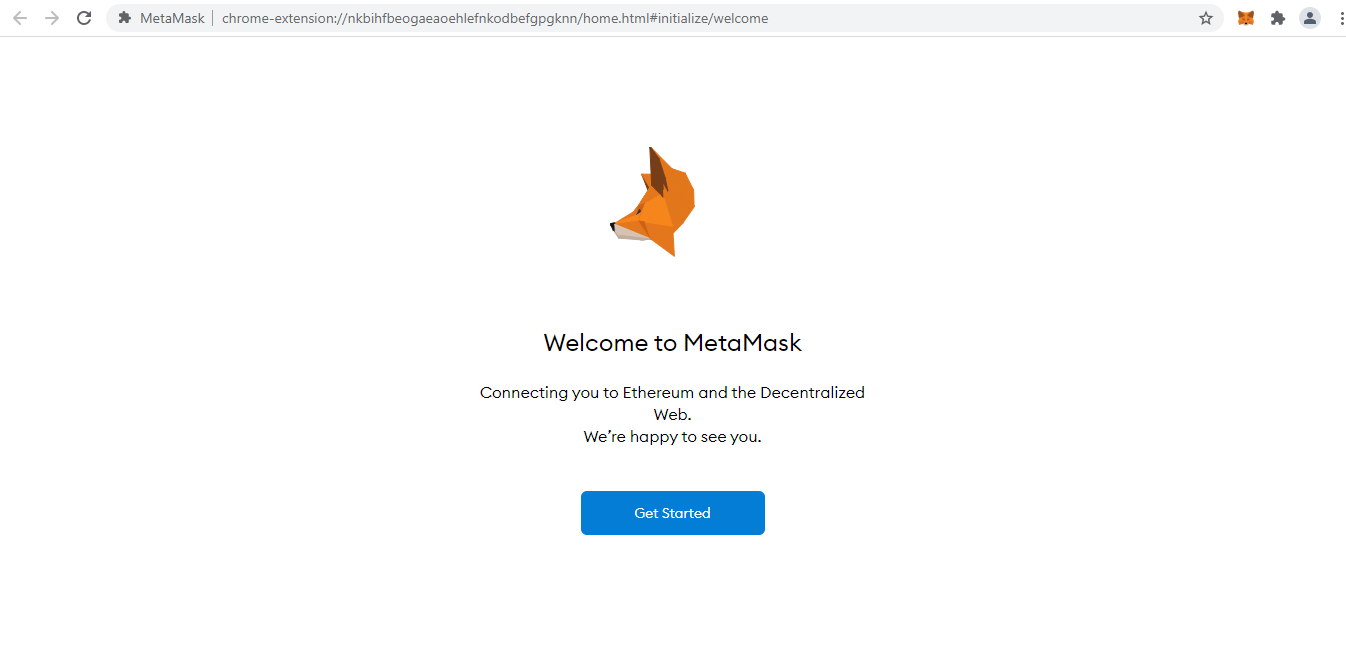
\includegraphics[scale=0.4]{metamask_getstarted.png}}
  \caption{Inicio para crear o importar una wallet, Fuente: captura de pantalla.}
  \label{img:metamask_getstarted}
\end{figure}

Como siguiente paso hay que crear una wallet. Esto es importante para poder interactuar con el sistema
(específicamente con los smart contract). Leer los términos y condiciones si están de acuerdo aceptarlos,
el siguiente paso es crear una contraseña, esta sirve para acceder a Metamask en el computador local, evita que otro usuario pueda acceder si no conoce la contraseña y agrega un nivel más de seguridad, ya que  se pueden realizar diferentes operaciones.

\begin{figure}[H]
  \centering
  {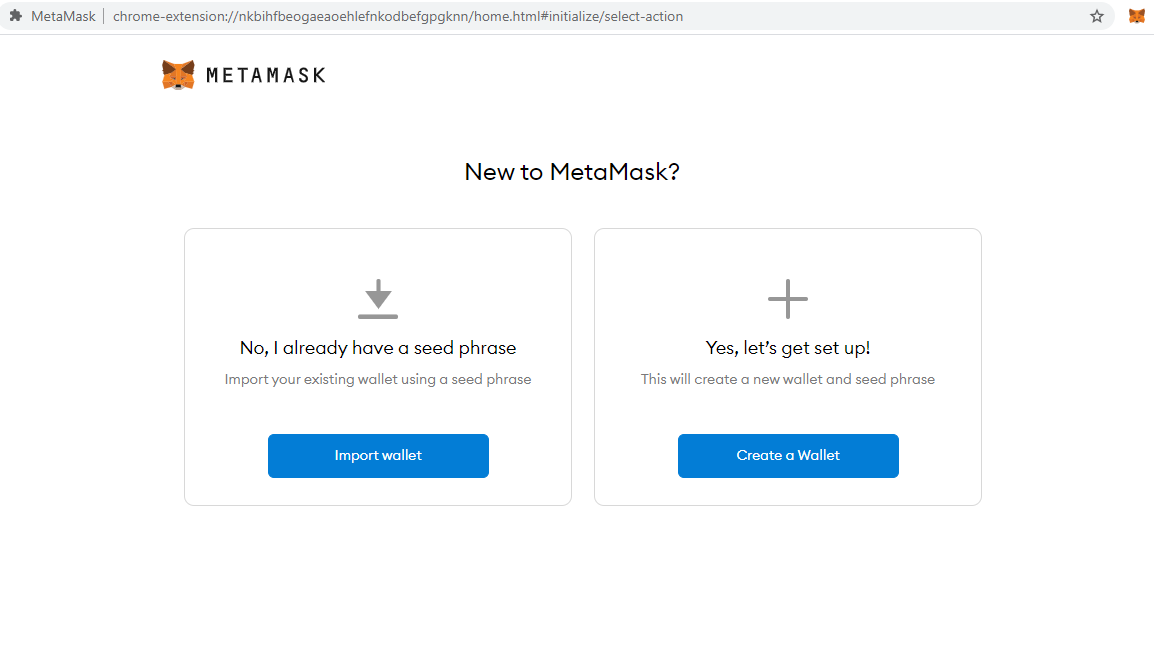
\includegraphics[scale=0.4]{metamask_create.png}}
  \caption{Menú crear wallet,  Fuente: captura de pantalla. }
  \label{img:metamask_create}
\end{figure}

\begin{figure}[H]
  \centering
  {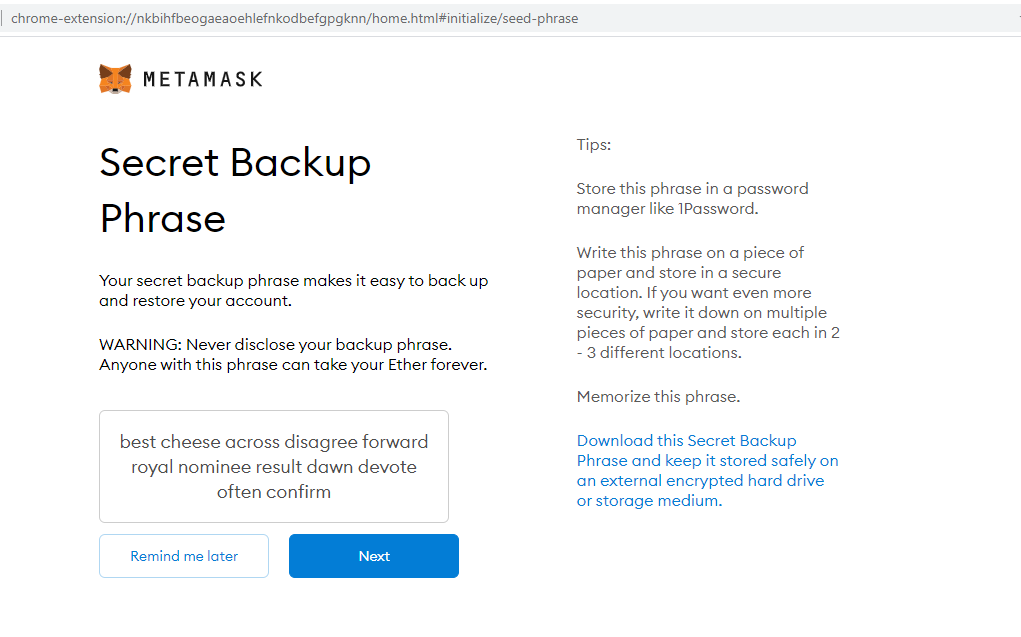
\includegraphics[scale=0.4]{metamask_semilla.png}}
  \caption{Frases semillas,  Fuente: captura de pantalla. }
  \label{img:metamask_semilla}
\end{figure}

Un vez ingresada la contraseña se mostrará su frase semilla de su wallet, 
Tal como se observa en la figura \ref{img:metamask_semilla}, la frase se muestra de modo didáctico 
pero la misma nuca debe ser compartida bajo ningún término, ya que el usuario
que conozca la frase semilla podrá abrir la wallet desde otro metamask y hacer lo que desee con ella,
la única manera que otro usuario no pueda intervenir o manejar su wallet es que no conozca la frase semilla, 
por ello es muy importante guardarla en un sitio que solo la personas dueña de la frase semilla conozca,  
a partir de esta frase se genera la llave privada.
La frase semilla generada para esta investigación será rechazada y se usarán otras.
Finalizada la creación de la wallet, se podrá fijar en la parte derecha como se muestra en la figura \ref{img:metamask_new}
\begin{figure}[H]
  \centering
  {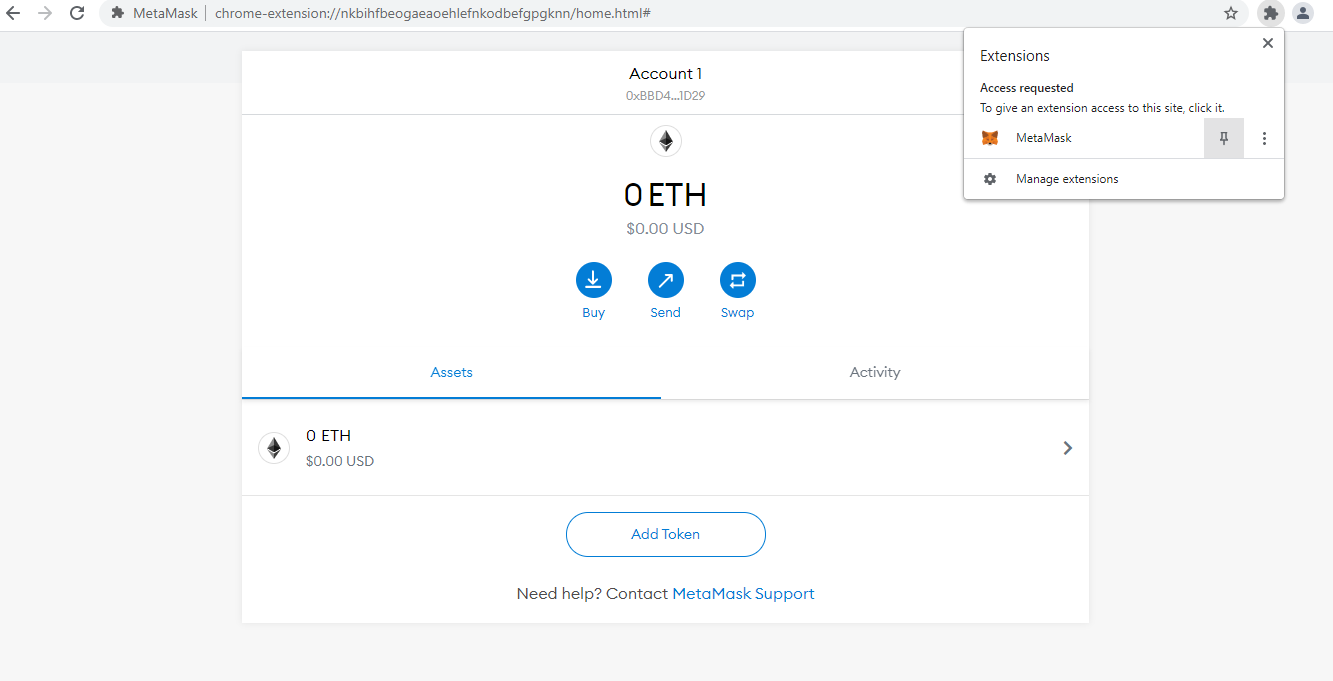
\includegraphics[scale=0.4]{metamask_new.png}}
  \caption{Creación de la wallet finalizada,  Fuente: captura de pantalla. }
  \label{img:metamask_new}
\end{figure}


\subsection{Desarrollo del Smart Contract}
Se utilizó Remix para  la edición del código fuente escrito en Solidity, este programa 
permite compilar el código para probarlo de manera local y también es una herramienta para publicarlo de manera online en otras Blockchain.
En este caso se publicó en Ropsten.

El código del smart contract se desarrolló siguiendo las definiciones de la sección \ref{s:system_design}, se encuentra en el anexo \ref{as:codigo_smart_contract}
En él se definieron los métodos ya mencionados y se agregaron reglas para que métodos en particulares puedan ser ejecutados solo por el propietario del smart contract y otros 
solo para los propietarios de las áreas.

El código desarrollado, cumple con los principios descriptos en otras secciones, 
y sigue algunas pautas de los estándares de certificados ya mencionados como BlockCerts y OpenCerts.
Algunas pautas son: almacenar información del emisor, almacenar el hash del documento, no relacionar datos
personales del propietario del documento digital.

 

% \begin{figure}[hbt!]
%   \centering
%   {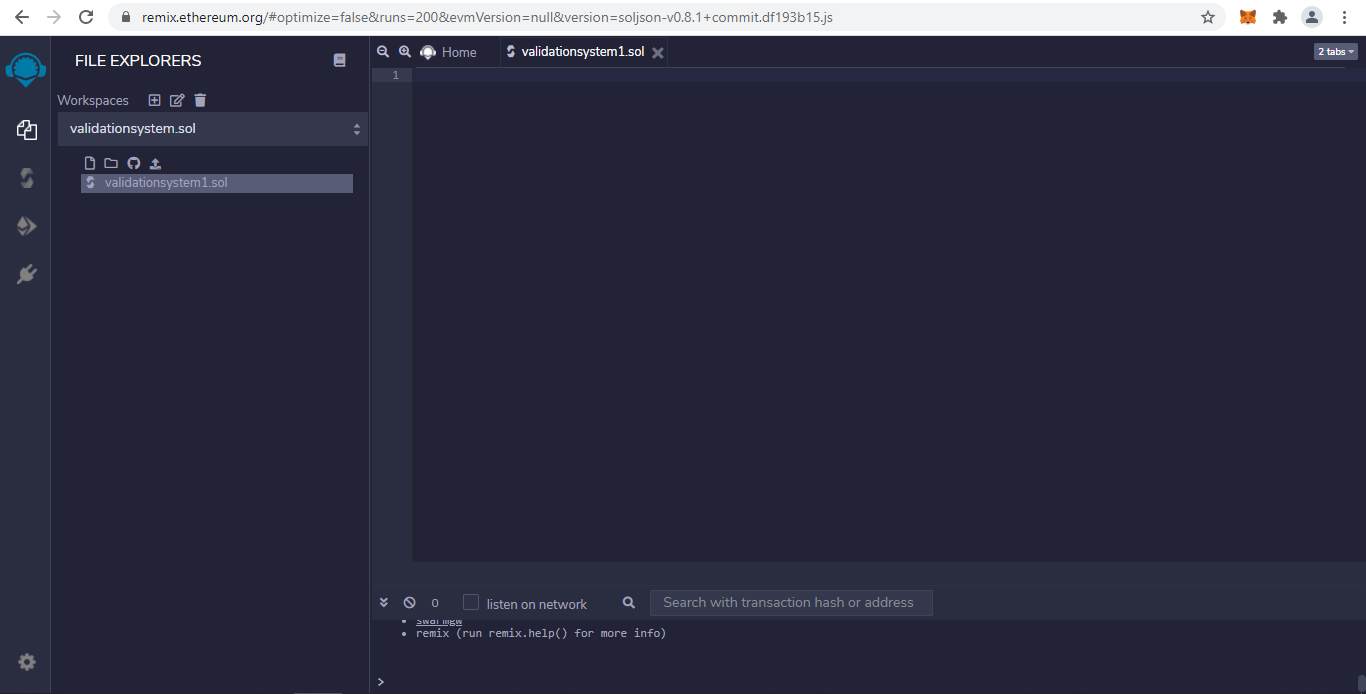
\includegraphics[scale=0.4]{validationSystem.png}}
%   \caption{Creando el smart contract con extensión “.sol”, Fuente: captura de pantalla. }
%   \label{img:valdationSystem}
% \end{figure}

Se desarrolla el código dentro del archivo “validationsystem.sol”, que tiene toda la lógica
del sistema con los comportamientos que se pueden realizar.
Una vez que el código está finalizado, hay que compilarlo, la figura   \ref{img:smart_contract_compile} muestra un ejemplo.
\begin{figure}[H]
  \centering
  {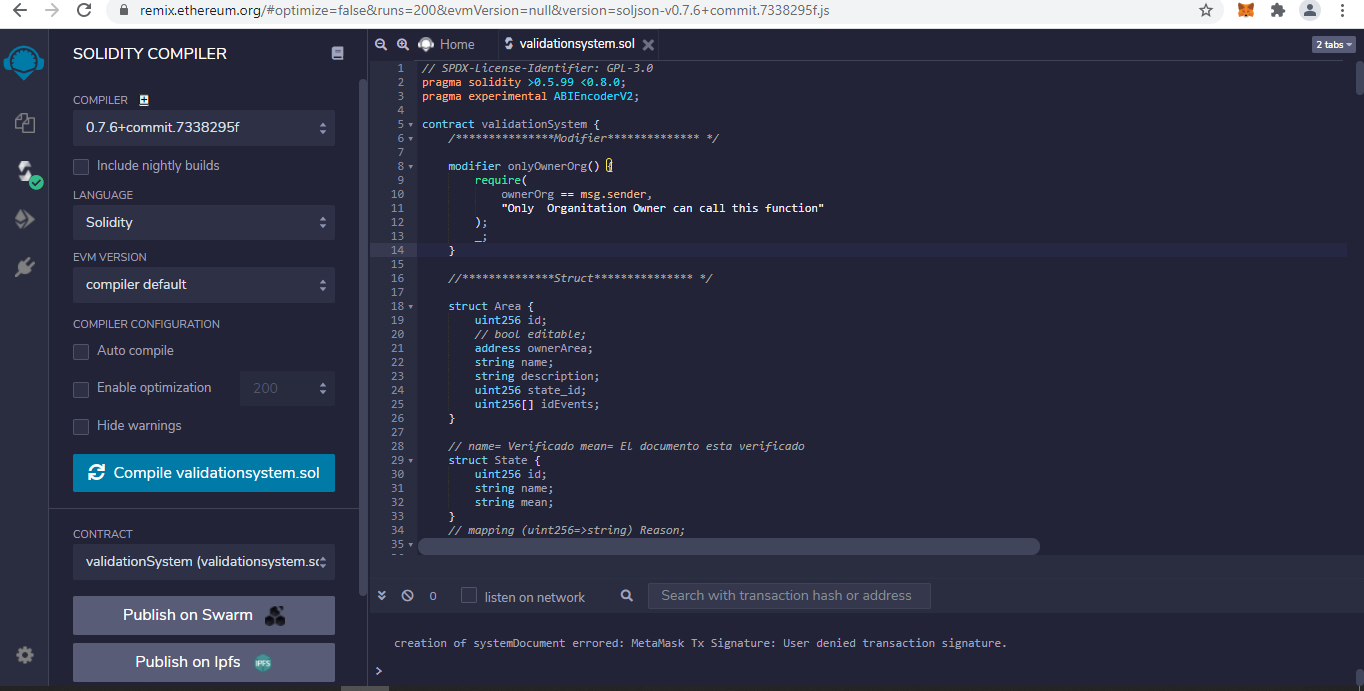
\includegraphics[scale=0.4]{smart_contract_compile.png}}
  \caption{Vista como compilar el contrato, Fuente: captura de pantalla. }
  \label{img:smart_contract_compile}
\end{figure}


Por otra parte es un requisito publicar el smart contract en alguna Blockchain, para ello hay que ejecutar Metamask y seleccionar la red de Ropsten 
como se muestra en la figura \ref{img:ropsten_selected}.
Luego es necesario conseguir la criptomoneda nativa de la Blockchain, 
para ello hay que acceder  a los sitios web denominados como \gls{faucet}, estos sitios 
web facilitan obtener las criptomonedas nativas. Para Ropsten se puede acceder al sitio web 
proporcionado por \href{https://faucet.metamask.io/}{Metamask}  o 
proporcionado por \href{https://faucet.ropsten.be/}{Ropsten} ambos sirven para obtener las criptomonedas para la red de prueba.  
\begin{figure}[H]
  \centering
  {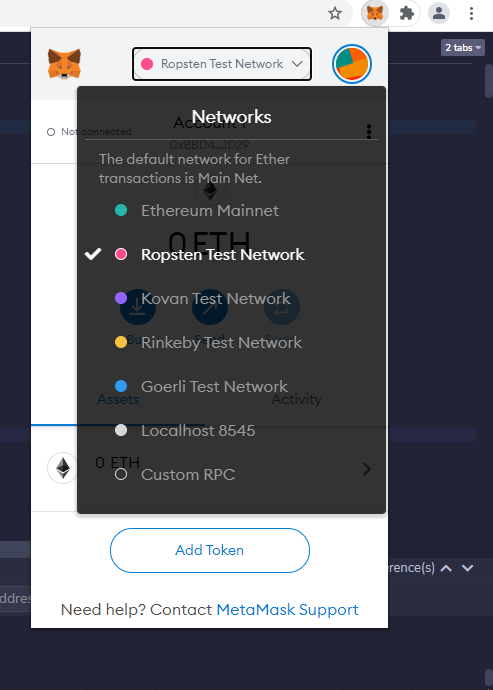
\includegraphics[scale=0.7]{Ropsten_seleteced.png}}
  \caption{Seleccionando la Red de Ropsten, Fuente: captura de pantalla. }
  \label{img:ropsten_selected}
\end{figure}

En este caso se utilizó el sitio web de la figura \ref{img:faucet_metamask} haciendo clic en el  botón verde,
suma 1 ETH a la cuenta.
\begin{figure}[H]
  \centering
  {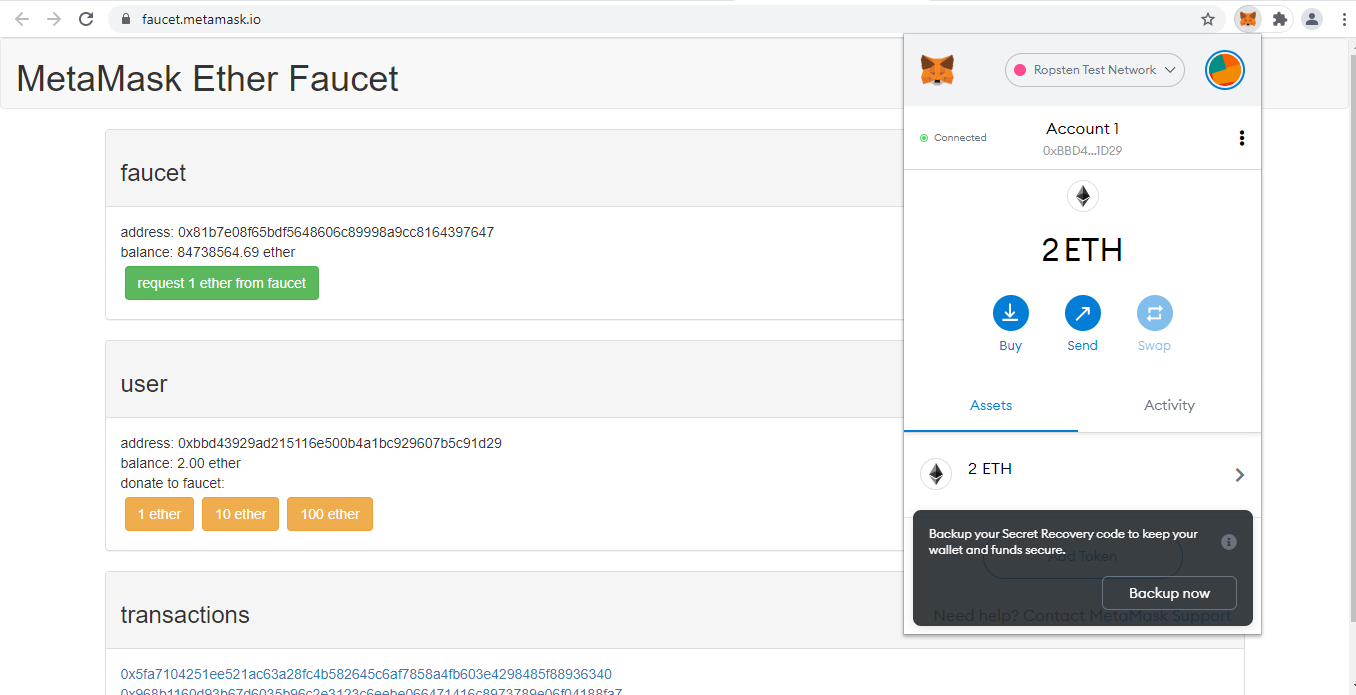
\includegraphics[scale=0.4]{FaucetMetamask.png}}
  \caption{Grifo de MetaMask, Fuente: captura de pantalla. }
  \label{img:faucet_metamask}
\end{figure}

A partir de ahora, se cuentan con todas las condiciones para publicar el código en la  Blockchain de Ropsten.
Para ello en el menú izquierdo de Remix  seleccionar la opción de  deploy, dentro de ella ir en la opción de “enviroment”  y seleccionar  “inject web3”, 
lo que abrirá Metamask requiriendo conectar la wallet con el sistema de Remix. Luego hacer clic al botón de color naranja (deploy) que se observa en la Figura \ref{img:remix_compile}

\begin{figure}[H]
  \centering
  {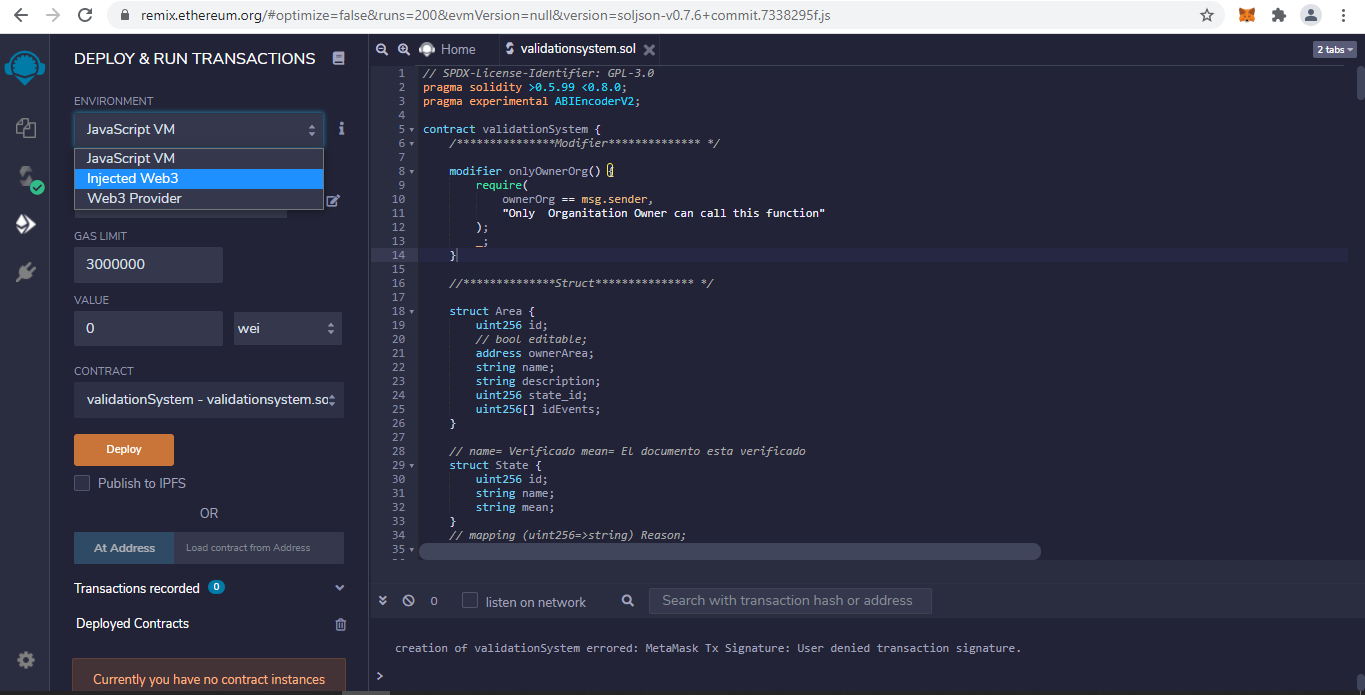
\includegraphics[scale=0.4]{remix_compile.png}}
  \caption{Menú deploy Remix, Fuente: captura de pantalla. }
  \label{img:remix_compile}
\end{figure}

\begin{figure}[H]
  \centering
  {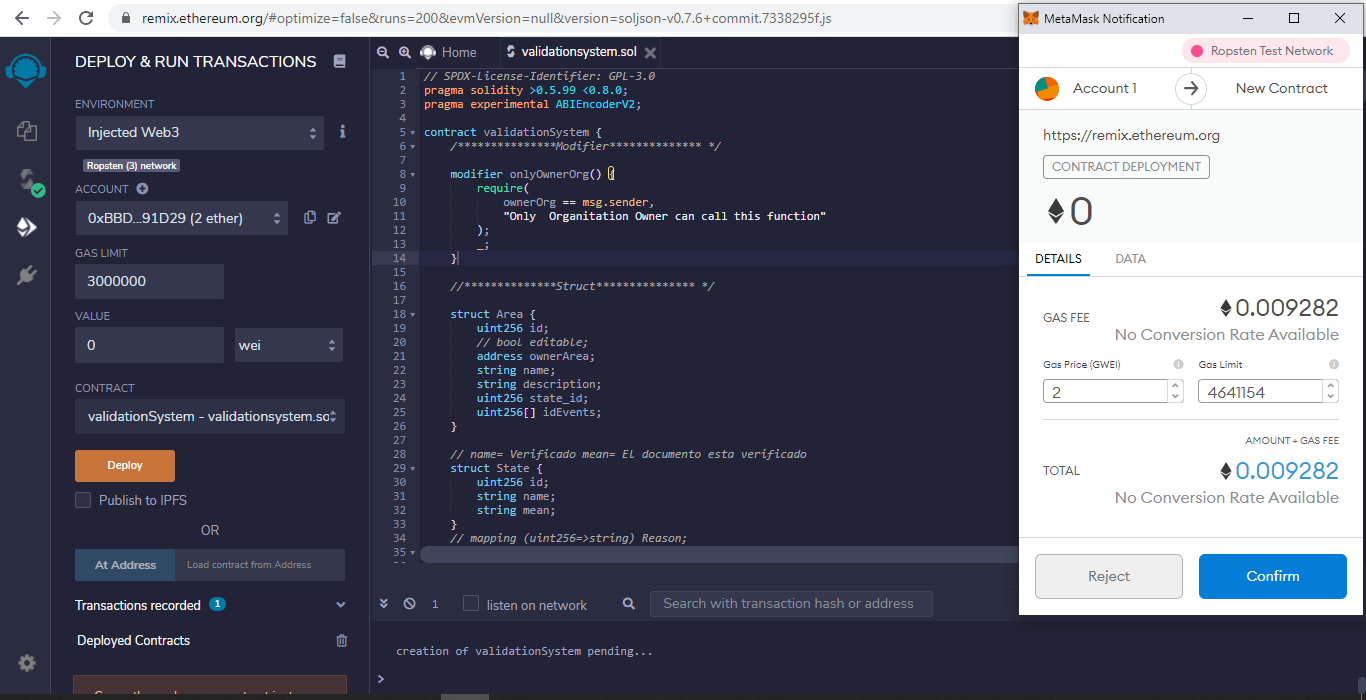
\includegraphics[scale=0.4]{remix_deploy.png}}
  \caption{Deploy Contrato Inteligente, Fuente: captura de pantalla. }
  \label{img:remix_deploy}
\end{figure}

Se abrirá una ventana de Metamask (Figura \ref{img:remix_deploy}), que pedirá la confirmación para gastar una cantidad de ETH, que es la criptomoneda
que se obtuvo mediante  la pagina web de grifo o faucet de Ropsten, la cual se utiliza para pagar las transacciones en la Blockchain.
Se confirma la transacción, y quedará en pendientes hasta ejecutarse, una vez finalizada el smart contract estará en la  Blockchain lista para
usarla.
En la figura \ref{img:metodos_contract_deploy} se muestran los métodos del contrato que se pueden ejecutar en la Blockchain, la interfaz
Remix también sirve para llamar a los diferentes métodos creados.
\begin{figure}[hbt!]
  \centering
  {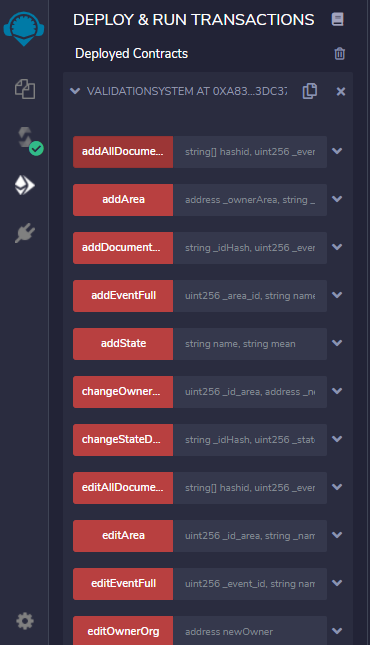
\includegraphics[scale=0.7]{Metodos_contract_deploy.png}}
  \caption{Contrato en la  Blockchain de Ropsten, Fuente: captura de pantalla. }
  \label{img:metodos_contract_deploy}
\end{figure}


\section{Desarrollo de la Interfaz de Usuario}
El desarrollo se realizó con el sistema operativo Windows 10 Home, pero
las herramientas pueden usarse en distribuciones de GNU/Linux.
Como primer paso se requiere instalar NODE JS desde su sitio oficial; también se utilizará Visual Studio Code como editor de texto.

Otro punto, es instalar  VUE JS CLI para facilitar la instalación de todos los paquetes y tener una estructura más organizada \cite[]{vue_cli_overview_2019},
para ello previamente se requiere instalar  NODE JS, en cmd o la consola de comandos del Visual 
Studio Code se ejecuta el comando “npm install -g @vue/cli”, para instalarlo de manera global,
en la figura \ref{img:INSTALL_VUE_CLI} se realiza utilizando Visual Studio Code.

\begin{figure}[H]
  \centering
  {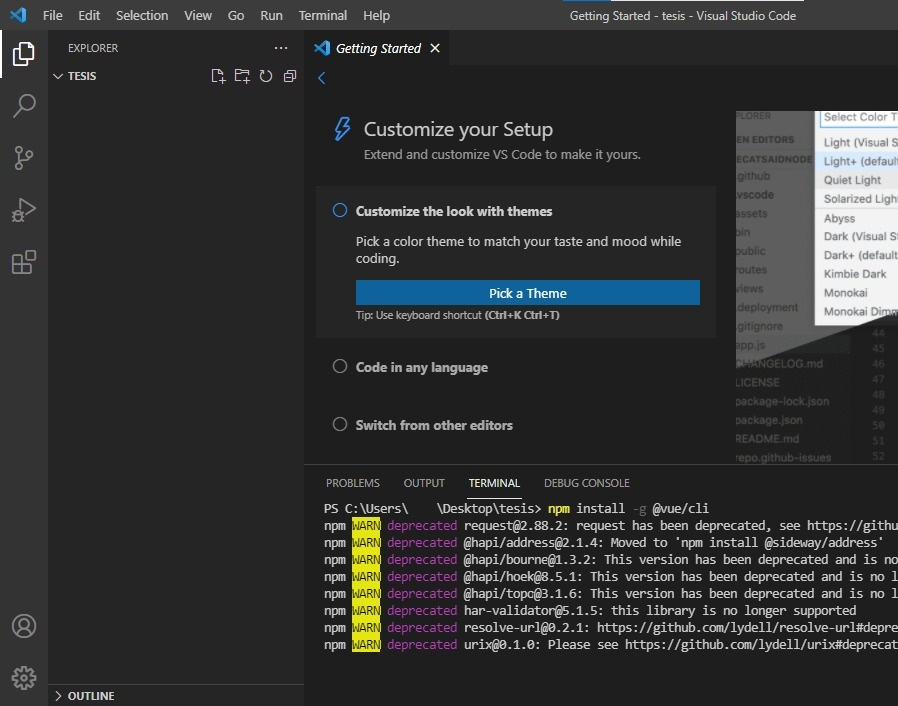
\includegraphics[scale=0.7]{INSTALL_VUE_CLI.jpeg}}
  \caption{Comando para instalar VUE CLI, Fuente: captura de pantalla. }
  \label{img:INSTALL_VUE_CLI}
\end{figure}

Luego en la consola de comandos hay que ubicarse en el directorio que se desea instalar el proyecto. Una vez hecho, ejecutar el comando 
“vue create nombre\_proyecto”, en este caso se usó “vue create validation\_system” esto abre unas opciones de configuraciones en consola, 
para el proyecto se utiliza router, vuex, babel; seleccionados estos ítems continuar con la instalación, en la figura \ref{img:vue_config} se muestra
las opciones necesarias para la creación del proyecto.
\newpage
\begin{figure}[H]
  \centering
  {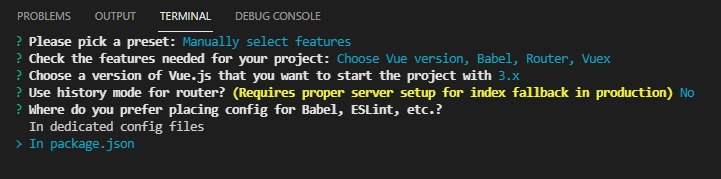
\includegraphics[scale=0.6]{VUE_Config.jpeg}}
  \caption{Configuración de proyecto, Fuente: captura de pantalla. }
  \label{img:vue_config}
\end{figure}

Como siguiente paso se debe ingresar dentro del directorio del proyecto creado en el cual se usarán dos librerías ya mencionadas ( web3 \cite[]{web3js_web3js_2016}, y sha256 \cite[]{satoh_asic-hardware-focused_2007}), 
también se usará un componente
que facilita la creación y carga de los select múltiples, mediante VUE. La instalación de estos se realiza con los comandos mostrados en la figura \ref{img:libreria}

\begin{figure}[hbt!]
  \centering
  {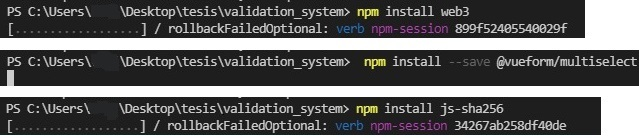
\includegraphics[scale=0.7]{librerias.jpeg}}
  \caption{Instalación de librerías y componente, Fuente: captura de pantalla. }
  \label{img:libreria}
\end{figure}

A partir de este punto comienza el desarrollo de la interfaz gráfica con las librerías y herramientas instaladas.

\subsection{Desarrollo de la Vista del Sistema}
Inicialmente, con la carpeta del proyecto generada se crean unos archivos extras, en este caso dentro de la ruta del proyecto “nombre\_proyecto/src/” se crea manualmente una carpeta con el nombre \/app donde
se almacenarán archivos que permitirán conectar con la Blockchain.

\begin{figure}[H]
  \centering
  {\includegraphics[scale=0.7]{ruta_archivo_Blockchain.png}}
  \caption{Archivos para conexión con la Blockchain, Fuente: captura de pantalla. }
  \label{img:ruta_archivo_Blockchain}
\end{figure}
El archivo abi.js define todos los métodos o funciones que se pueden usar en el smart contract creado, y  para eso 
hay que dirigirse a Remix, compilar nuevamente el código del smart contract y copiar el \gls{abi} creado. Por ejemplo, 
en la figura \ref{img:abi_copy} se resalta con un circulo rojo, el botón para copiar el \gls{abi}; este código se almacena 
dentro del archivo abi.js, ya que es utilizada para  las llamadas a los métodos.

\begin{figure}[H]
  \centering
  {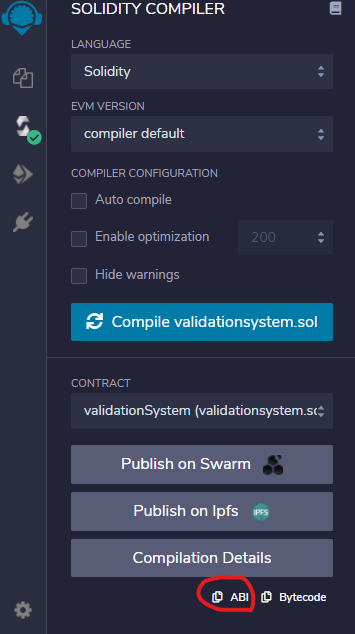
\includegraphics[scale=0.7]{ABI_Copy.png}}
  \caption{Copiar el ABI del código, Fuente: captura de pantalla. }
  \label{img:abi_copy}
\end{figure}

Posteriormente se crean una serie de archivos como app.js, document.js, parameters.js que contendrán la lógica para conectar la vista frontal con la Blockchain.
El último archivo parameters.js almacena la dirección del smart contract, la dirección se crea en el momento que se publicó el código con Remix,
la dirección generada es “\textbf{0x7006882779C21D8246 C82989F813237f78A781b1}”.


Las vistas desarrolladas  con VUE JS:
\begin{enumerate}
  \item \textit{Gestión de Área}: permite crear  Áreas, asignar un propietario mediante una dirección o clave pública, un nombre, descripción,
  a partir de él se pueden crear eventos.

  \begin{figure}[H]
    \centering
    {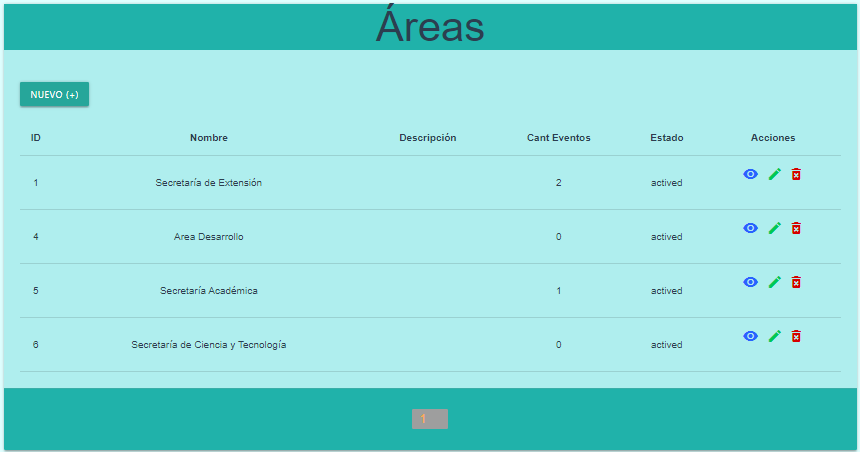
\includegraphics[scale=0.7]{Front_Area.png}}
    \caption{Vista de Áreas,  Fuente: captura de pantalla. }
    \label{img:front_area}
  \end{figure}

  \item \textit{Gestión de Evento}: se crean los Eventos encargados de generar los documentos, los datos para crear un evento son el nombre, 
  área relacionada, descripción, fecha de cuando inicio el evento, fecha cuando finaliza el evento y un estado. 
  Las fechas sirven para saber en que período se crearon los documentos, ya que cada documento está relacionado  a un evento.
  
  \begin{figure}[H]
    \centering
    {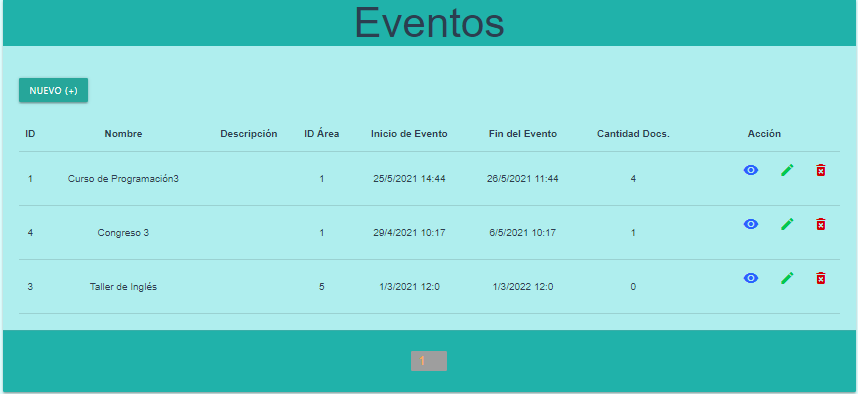
\includegraphics[scale=0.7]{Front_event.png}}
    \caption{Vista de Eventos,  Fuente: captura de pantalla. }
    \label{img:front_event}
  \end{figure}     
  
  \item \textit{Gestión de Documentos}: Se verifican o validan los documentos, si el usuario tiene el rol para crear documentos 
  también se utiliza como carga del mismo, si no tiene un rol solamente puede verificar si el documento fue registrada por la organización. 
  Un usuario propietario del área ve como se muestra en la figura \ref{img:front_document_owner}.

  \begin{figure}[H]
    \centering
    {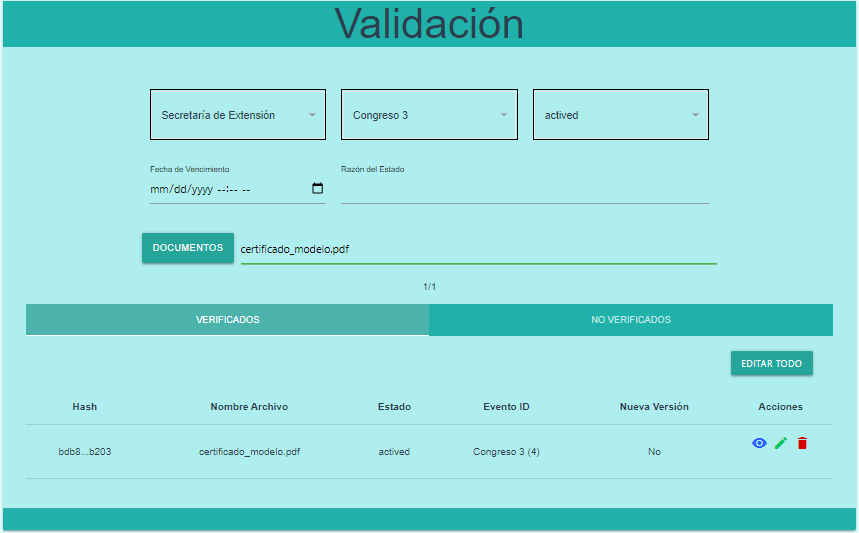
\includegraphics[scale=0.7]{Front_document_owner.png}}
    \caption{Vista de Documentos como propietario,  Fuente: captura de pantalla. }
    \label{img:front_document_owner}
  \end{figure}
  Y en el caso de una dirección pública que 
  no está registrada como propietario de un área o de la organización visualiza los documentos como en la figura \ref{img:front_document_public}.
  \begin{figure}[H]
    \centering
    {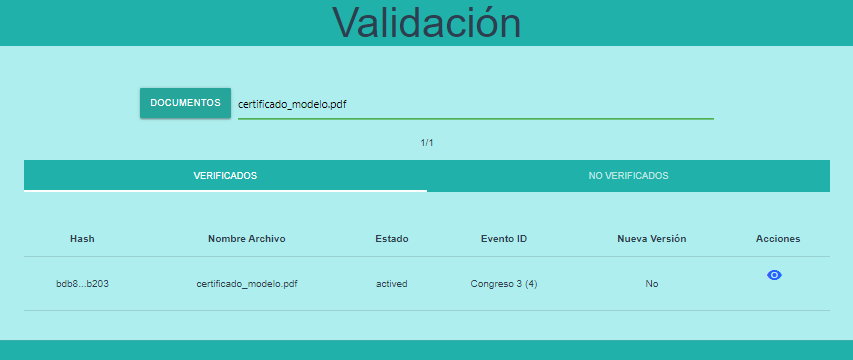
\includegraphics[scale=0.7]{front_document_public.png}}
    \caption{Vista de Documentos como usuario público,  Fuente: captura de pantalla. }
    \label{img:front_document_public}
  \end{figure}

  \item \textit{Gestión de Organización}: Mantiene los datos de la Organización, permite cambiar el nombre, cargar nuevos estados y cambiar al propietario de la organización, que 
  en este caso es el usuario que tiene permitido todas las acciones creadas.
  Los estados cargados por defecto son “deleted”, “actived”, “expired” y no pueden ser eliminados en el sistemas  ni modificados excepto “expired”. 

  \begin{figure}[H]
    \centering
    {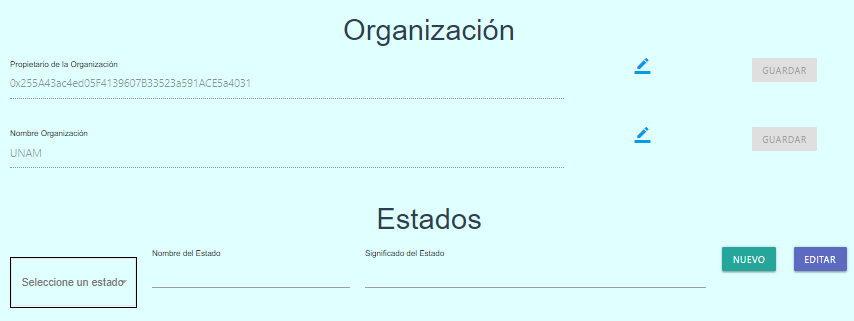
\includegraphics[scale=0.7]{front_org.png}}
    \caption{Vista de Organización,  Fuente: captura de pantalla. }
    \label{img:front_org}
  \end{figure}
\end{enumerate}


% El código completo del front end se encuentra en el repositorio de git \footnote{\url{https://github.com/agustinbritez/Sistema_Validacion.git}}.

%%%-------------------------Ensayos  validacion------------------------
\chapter{Ensayos de Validaciones} \label{c:ensayo_validacion}
Los ensayos se realizarón con certificados emitidos por la  Secretaría de Extensión de la \gls{fce} de la \gls{unam}, por una cuestión
de conveniencia en el acceso de los documentos digitales de la Universidad, pero los ensayos se podrían realizar sin importancia del área.


El ensayo inicia con la cuenta o dirección del propietario del smart contract, quien  carga los datos base, como el nombre de la Organización, las áreas, los eventos en donde se emitirán los certificados.
Partiendo de un smart contract desplegado como se muestra en otras secciones, el administrador o propietario de la organización es la misma   dirección que se encargó  
de publicar el contrato inteligente, pero el usuario administrador puede cambiar su dirección por otra.
\section{Preparación Inicial}
Los siguientes pasos se realizan con la cuenta del propietario del Smart Contract.
Primero se ingresa el nombre de la organización a “Universidad Nacional de Misiones Facultad de Ciencias Económicas”, esto sirve para identificar el nombre de la organización 
que es dueño del Smart Contract, se 
crean estados nuevos como “en espera”, “on hold” \ref{img:cambio_org}.
Se crean las Áreas de la Organización, es este caso “Secretaría de Extensión”, con el propietario del área con dirección  “0x255A43ac4ed05F41396 07B33523a591ACE5a4031”
y el estado “actived”, conforme a la figura \ref{img:nuva_area}. El propietario del área puede crear las actividades o eventos y realizar la validación de los 
documentos.

\begin{figure}[H]
  \centering
  {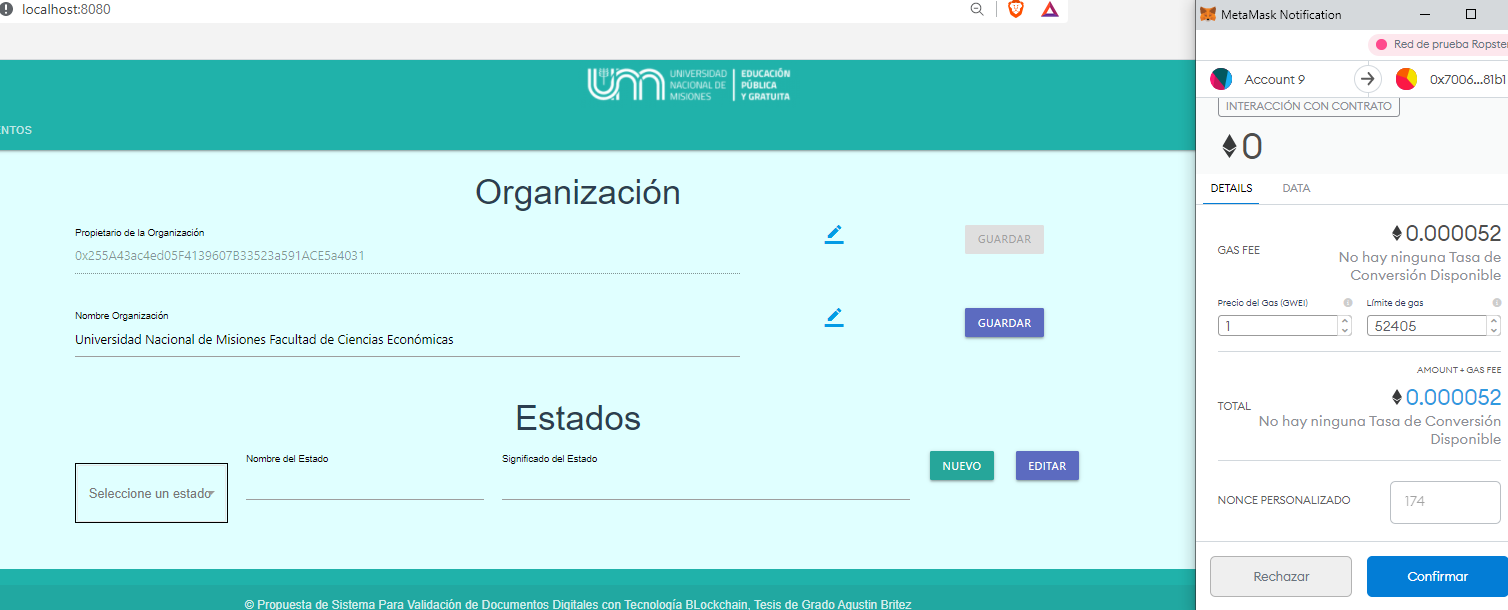
\includegraphics[scale=0.4]{cambio_organizacion.png}}
  \caption{Cambio de nombre de la organización,  Fuente: captura de pantalla. }
  \label{img:cambio_org}
\end{figure}

\begin{figure}[H]
  \centering
  {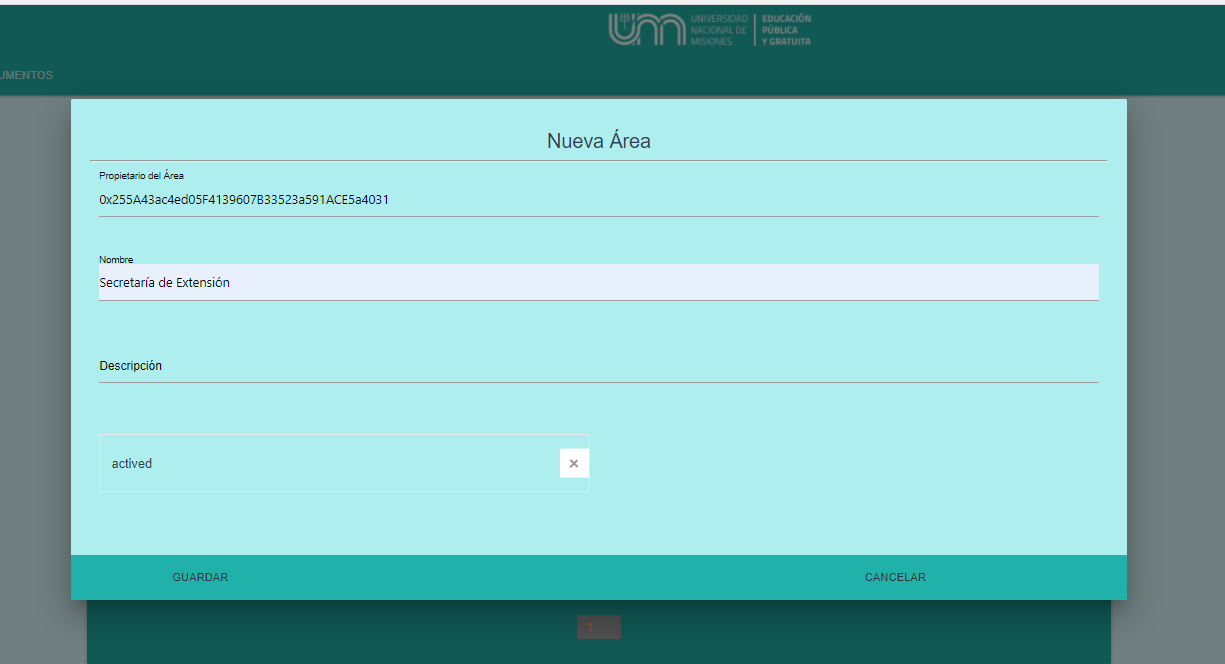
\includegraphics[scale=0.4]{nueva_area.png}}
  \caption{Creación de nueva área en el sistema,  Fuente: captura de pantalla. }
  \label{img:nuva_area}
\end{figure}


Se  crean los  eventos “Fondos Buitres”, “Geogebra” y “Taller  Liquidación”, que se relacionan al área recién mencionada que es 
“Secretaría de Extensión”.
% \begin{figure}[H]
%   \centering
%   {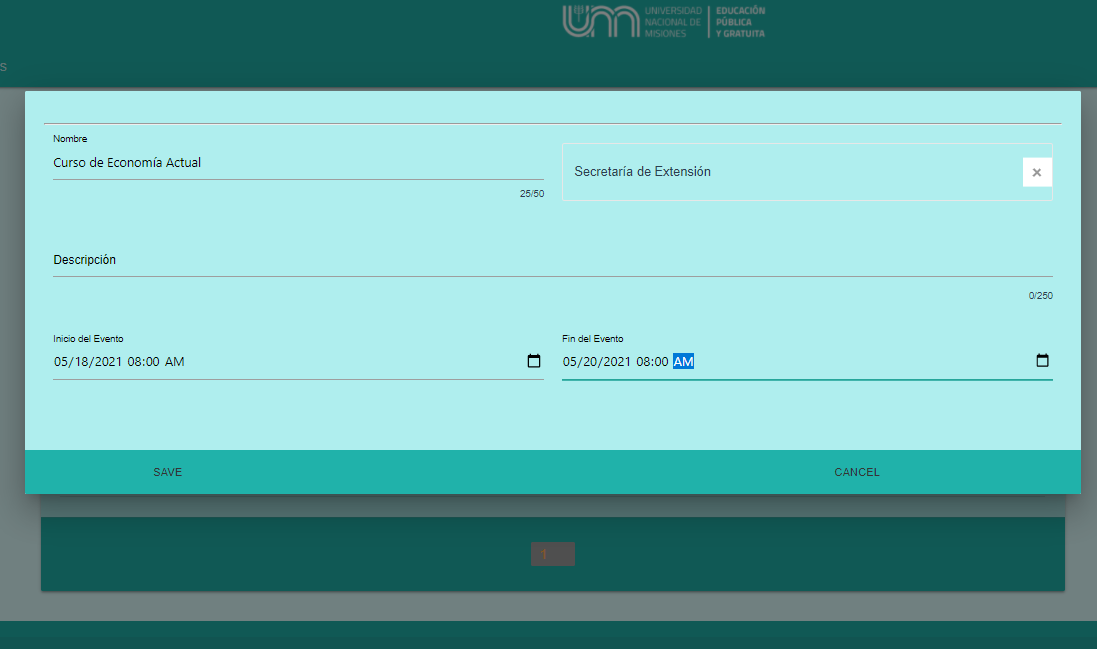
\includegraphics[scale=0.4]{nuevo_evento.png}}
%   \caption{Creación de nueva área en el sistema,  Fuente: captura de pantalla. }
%   \label{img:nuevo_evento}
% \end{figure}


Los ensayos serán realizados con la cuenta del propietario del Smart Contract.

\section{Ensayo A}
Se ensayó en un flujo habitual de la Secretaría de Extensión de la \glsfirst{fce}, 
siguiendo los circuitos normales de una actividad realizada por esta área. En base a la información recaudada en la entrevistas (A.L., comunicación personal, 02/10/2020),
  comenzando el flujo desde el momento que se crea un documento digital para entregar 
al participante de una actividad.

Una vez que el evento haya finalizado y se deben entregar los certificados, estos tiene que ser subidos al sistema de validación de la siguiente manera.
%%aca explicar con el primer certificado como se sube y en que vista o roles estoy
\begin{figure}[H]
  \centering
  {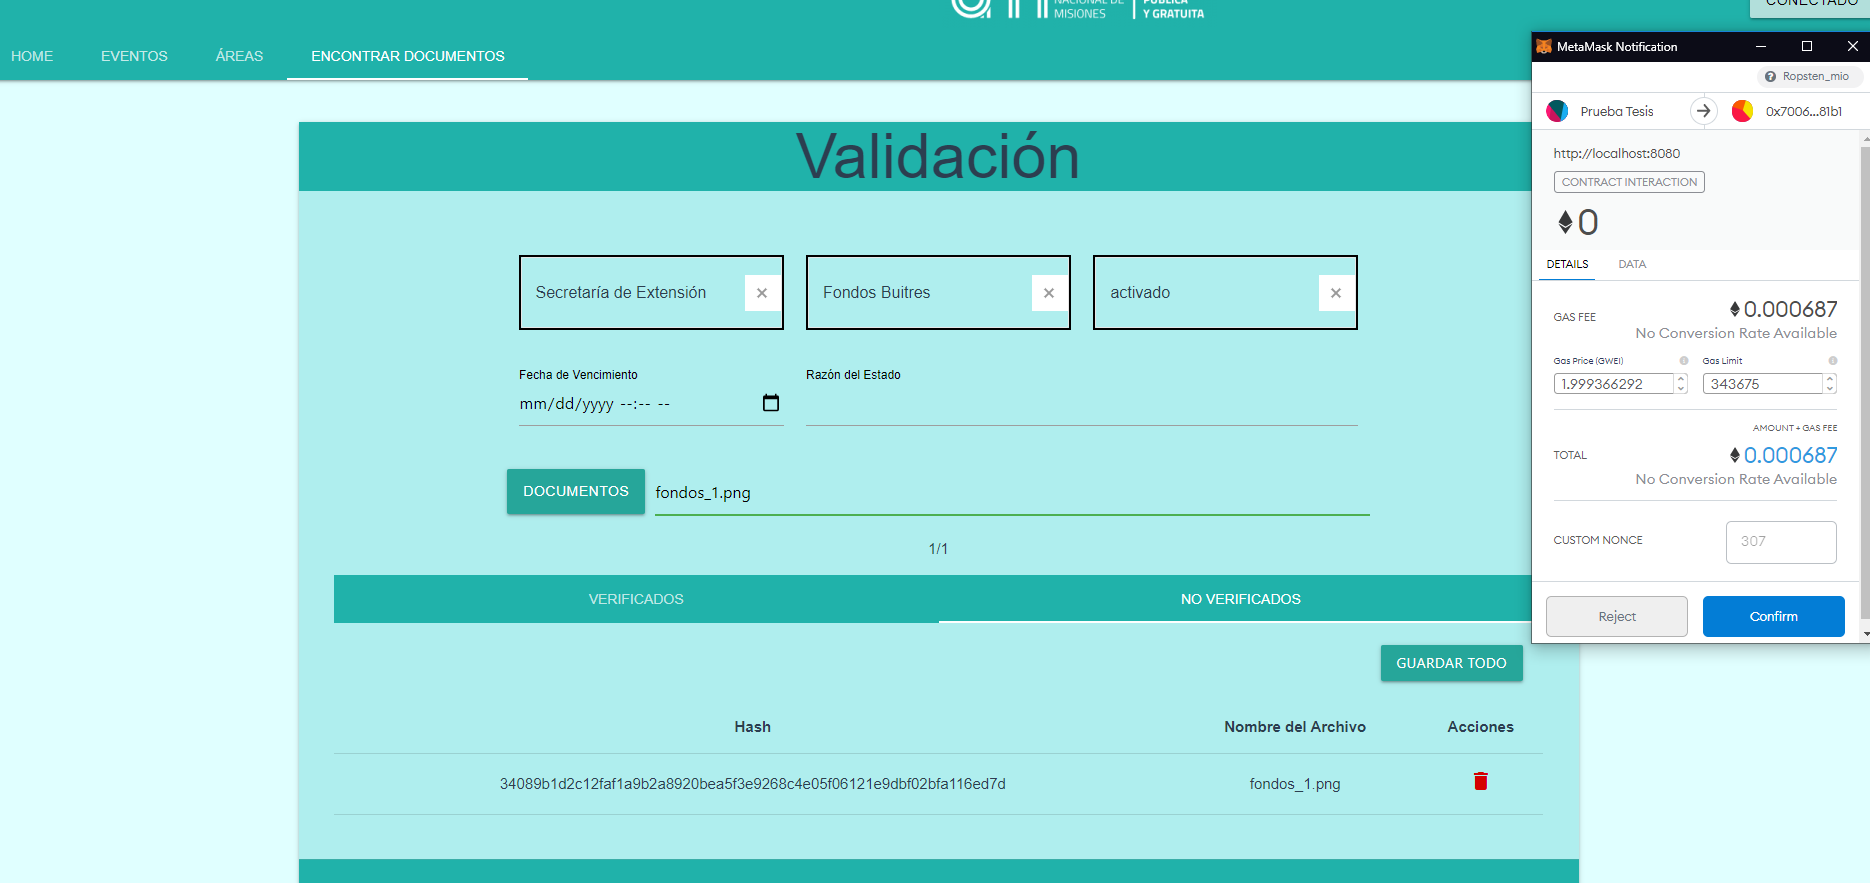
\includegraphics[scale=0.3]{paso_1_subir_documento.png}}
  \caption{Carga de certificado Fondos Buitres,  Fuente: captura de pantalla. }
  \label{img:paso_1}
\end{figure}

\begin{enumerate}
  \item Ingresar al sistema con la cuenta de administrador del área que organiza el evento y dirigirse a la vista “encontrar documento”, en la parte superior del sistema se puede observar en la figura \ref{img:paso_1}.
  \item Seleccionar el área que en este caso es la Secretaría de Extensión.
  \item Seleccionar el evento, en el caso actual es Fondos Buitres y seleccionar el estado que se requiere para los documentos a subir, por ejemplo  el estado “activado”.
  \item Hacer clic en el botón  “documentos” y se busca el certificado a subir en este caso es llamado fondos\_1.png, el certificado se muestra en la figura \ref{img:fondos_1}.
  \item En la figura \ref{img:paso_1} muestra el momento antes de generar el hash y almacenarlo en la Blockchain, cuando el propietario del área presiona el botón “GUARDAR TODO”,el sistema
  genera el hash de  los documentos
  seleccionados que están en la parte de “NO VERIFICADOS” y lo almacena en la Blockchain.
  \item A partir del punto cualquier individuo que consulte la Blockchain podrá verificar que el certificado actual fue emitido por la Secretaría de Extensión de la \gls{fce}. 
\end{enumerate}

\begin{figure}[H]
  \centering
  {
\includegraphics[scale=0.5]{Certificados Originales/fondos_1.png}}
  \caption{Certificado Original de fondos buitres,  Fuente: captura de pantalla. }
  \label{img:fondos_1}
\end{figure}

En el caso que un interesado desea comprobar que el PDF o documento que esta tiene en su poder fue emitido por la Secretaría de Extensión de la \gls{fce} de la \gls{unam}.
Debe ingresar al sistema en el caso de no ser propietario del área o del smart contract la vista aparece como la figura \ref{img:front_document_public},
luego seleccionar el botón “DOCUMENTOS” y subir el certificado que se quiere validar que es fondos\_1.png 

\begin{figure}[H]
  \centering
  {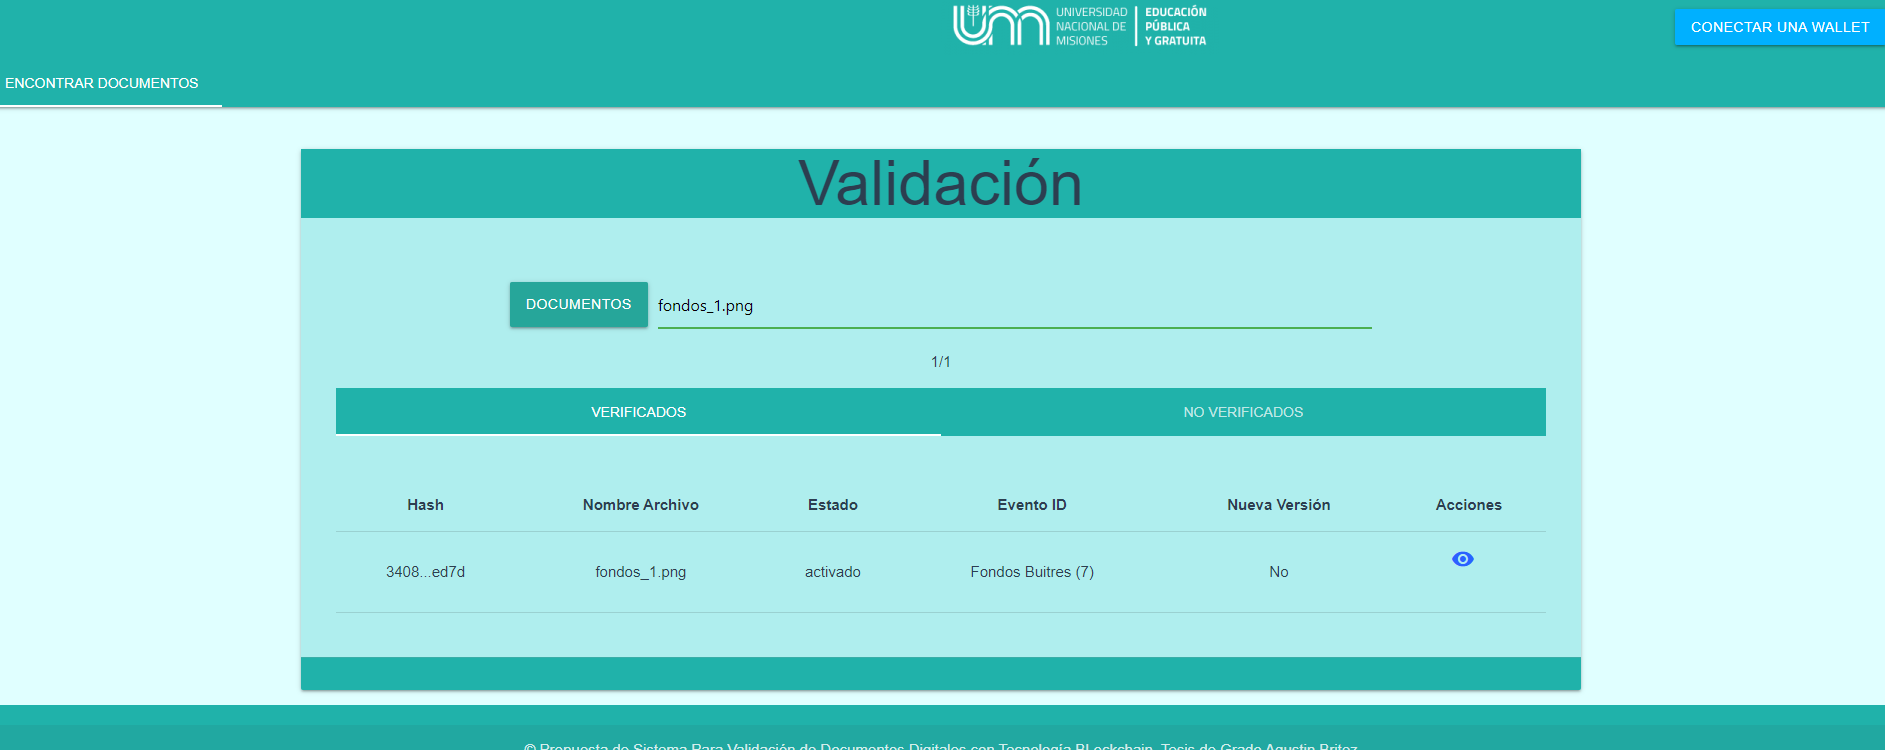
\includegraphics[scale=0.3]{fondos_buitres_captura_verificado.png}}
  \caption{Confirmación que el certificado se encuentra en la blockchain,  Fuente: captura de pantalla. }
  \label{img:fondos_1_verificado}
\end{figure}

Sí una persona intenta modificar el certificado para sus propios beneficios o para 
ocasionar algún tipo de daño de reputación u otro caso, el sistema se encargará de separar los certificados que no fueron emitidos
por una cuenta de propietario de  área de la \gls{fce} o del propietario del smart contract. A continuación el certificado de la figura \ref{img:fondos_1} fue modificado como se muestra en la 
figura \ref{img:fondos_1_alterado} se cambió el nombre del participante del evento a “Dr Ezequiel Britez DNI 00.134.321” (el nombre y el DNI del nuevo participante son
arbitrarios y ficticios). Este es un posible caso el cual una persona necesite un certificado con características esenciales para ella y modifique 
el documento a su voluntad.

\begin{figure}[H]
  \centering
  {
\includegraphics[scale=0.5]{Certificados Originales/fondos_1_alterado.png}}
  \caption{Certificado Fondos Buitres Modificado,  Fuente: captura de pantalla. }
  \label{img:fondos_1_alterado}
\end{figure}

En el caso que el certificado sea presentado, a una entidad podrá verificar  
que los datos
del certificado son correctos. Para ello la entidad debe acceder al sistema y realizar el 
mismo ya explicado, el cual es subir el documento
con el botón “DOCUMENTOS” de la vista. Para saber que el certificado o documento mantiene su información inalterable y que es emitida por la \gls{fce} de la \gls{unam},
el hash del certificado aparece en la sección “VERIFICADOS” como se muestra en la figura \ref{img:fondos_1_modificado_validacion}.

\begin{figure}[H]
  \centering
  {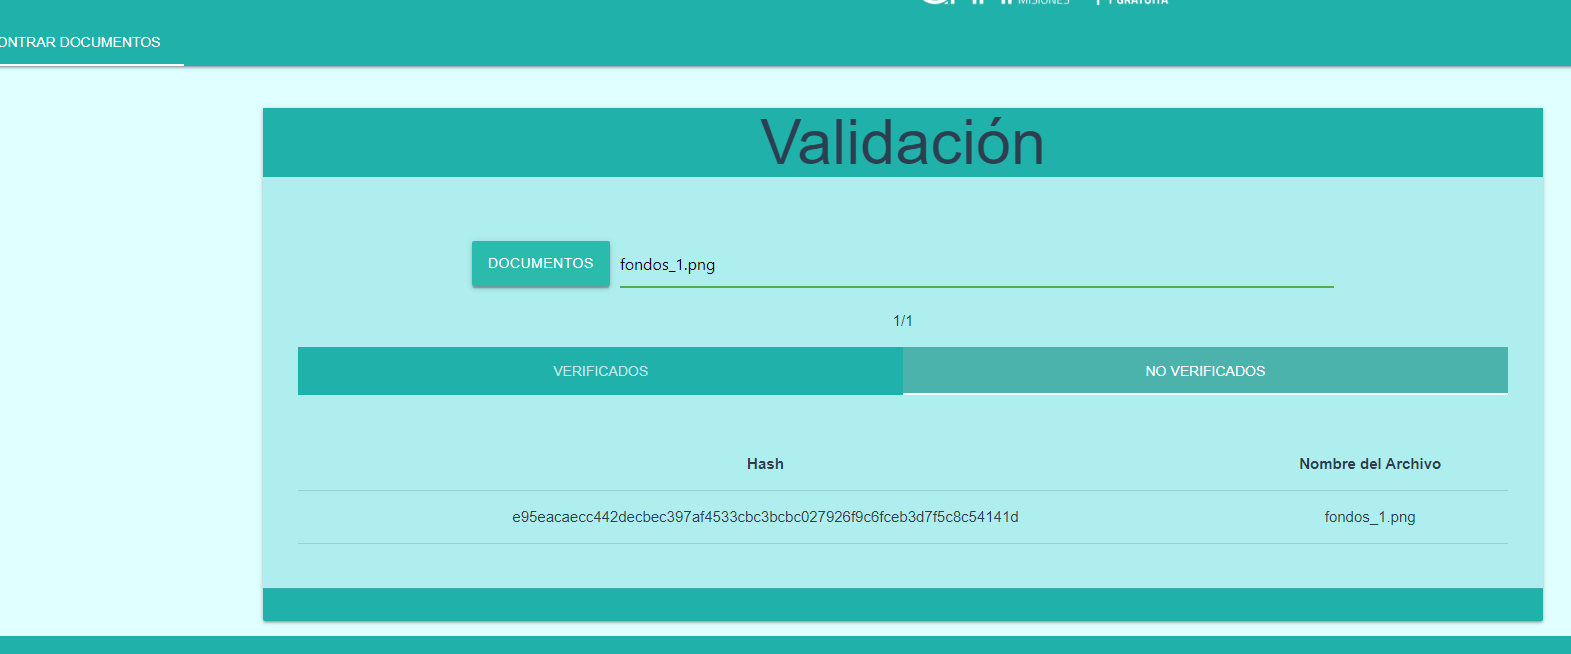
\includegraphics[scale=0.4]{fondos_1_prueba_modificado.png}}
  \caption{Validación de certificado modificado,  Fuente: captura de pantalla. }
  \label{img:fondos_1_modificado_validacion}
\end{figure}

Como se puede observar la tabla  \ref{table:tabla-ensayo-a} el hash del documento modificado es distinto al documento original.

\begin{table}[H]
  \centering
  % l = lefht c=centrado r=right
  \begin{tabular}{ |l|l|l| }
  \hline
  Hash Original & Hash Modificado & Cambia \\
  \hline
  34089b1d2c12faf1a9b2a8920 & e95eacaecc442decbec397af  &    \\
  bea5f3e9268c4e05f06121e9d & 4533cbc3bcbc027926f9c6fc  & SI \\
  bf02bfa116ed7d            & eb3d7f5c8c54141d          &    \\
  \hline
  \end{tabular}
  \caption{Comparación de los hash del certificado original \ref{img:fondos_1} y el modificado \ref{img:fondos_1_alterado}  }
  \label{table:tabla-ensayo-a}
  \end{table}

El resultado son distintos hashes porque los bits de cada documento son distintos \cite[]{back_hashcash_2002,nakamoto_bitcoin_2008,blockcerts_faq_nodate}. 

\section{Ensayo B}
Se sometió a prueba el certificado  (Certificado\_Geogebra.png de la figura \ref{img:certificado_geogebra}),
donde se cargan los datos Área: Secretaría de Extensión, Evento: Geogebra y Estado: Activado.
Y de la misma manera que el Ensayo A se carga el documento y confirma la transacción.

\begin{figure}[H]
  \centering
  {
\includegraphics[scale=0.5]{Certificados Originales/Certificado_Geogebra.png}}
  \caption{Certificado de participación curso Geogebra,  Fuente: captura de pantalla. }
  \label{img:certificado_geogebra}
\end{figure}

Es observable  en la figura \ref{img:geogebra_validado} que el certificado se subió correctamente y el hash se genero.

\begin{figure}[H]
  \centering
  {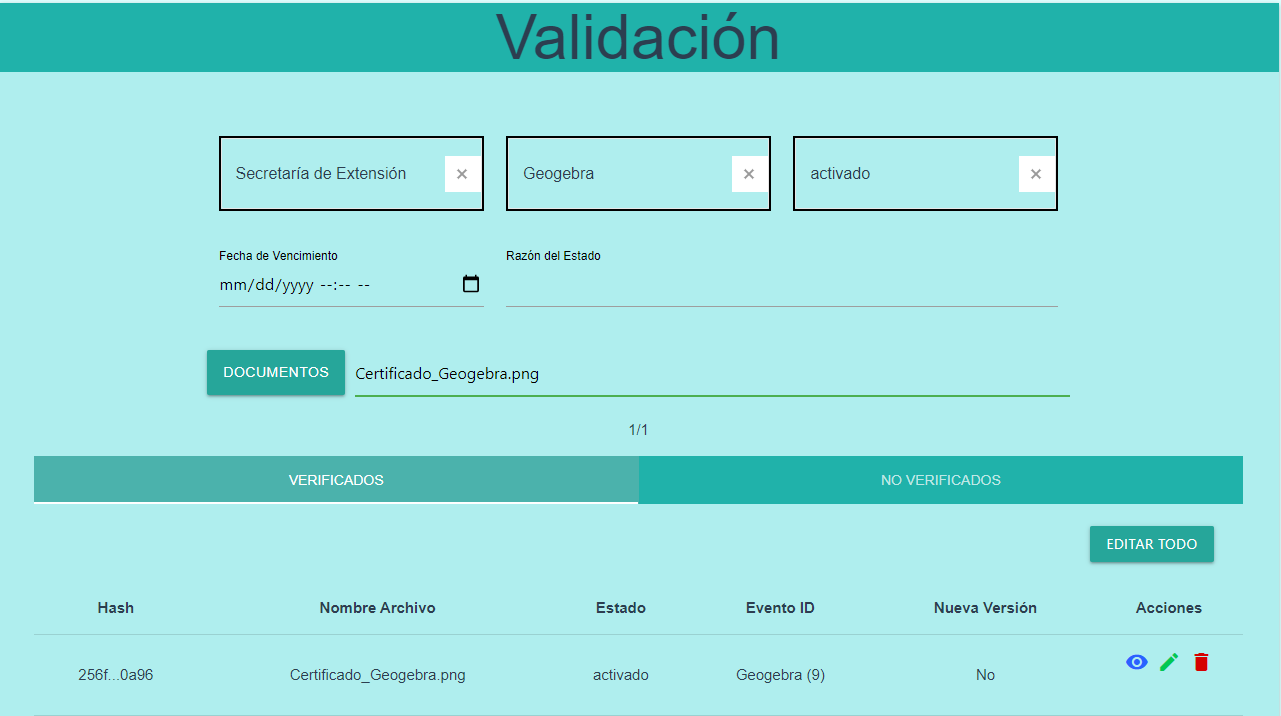
\includegraphics[scale=0.5]{geogebra_validado.png}}
  \caption{Certificado de Geogebra Validado,  Fuente: captura de pantalla. }
  \label{img:geogebra_validado}
\end{figure}

Como prueba se cambió el nombre del archivo de Certificado\_Geogebra.png a Bartolomeo\_Certificado\_Geo.png (ver Figura \ref{img:geogebra_cambio_nombre}) 
y se sometió al sistema 
para conocer si la integridad del certificado cambió. 

El  certificado aparece en la sección “VERIFICADOS” tras cambiar el nombre del archivo y probarlo. El sistema 
verifica que el hash del documento no 
se modificó porque internamente no sufrió cambios, esto permite  realizar modificaciones en el nombre del documento y no alterar a la validación.

\begin{figure}[H]
  \centering
  {\includegraphics[scale=0.5]{geo_cambio_nombre.png}}
  \caption{Cambio de nombre del Certificado,  Fuente: captura de pantalla. }
  \label{img:geogebra_cambio_nombre}
\end{figure}

A continuación se realiza una modificaciones internas  del Certificado\_Geogebra.png y el resultado se muestra en la figura  \ref{img:geogebra_alterado}

\begin{figure}[H]
  \centering
  {\includegraphics[scale=0.5]{Certificados Originales/Geogebra_1_alterado.png}}
  \caption{Certificado de Geogebra No Validado,  Fuente: captura de pantalla. }
  \label{img:geogebra_alterado}
\end{figure}

En la figura \ref{img:geogebra_alterado} se modificó el año del evento,  en algunas ocasiones las personas requieren
demostrar que realizó una capacitación o que tienen las habilidades que el certificado
demuestra. O cuando necesitan tener años de experiencias podría ocurrir un cambio de fechas.

Se probó el certificado modificado con el mismo nombre archivo pero este último no afecta al cálculo del hash. La prueba se muestra en
la figura \ref{img:geogebra_alterado_prueba} 

\begin{figure}[H]
  \centering
  {\includegraphics[scale=0.4]{geo_validacion_alterado.png}}
  \caption{Certificado de Geogebra Validado,  Fuente: captura de pantalla. }
  \label{img:geogebra_alterado_prueba}
\end{figure}

Como resultado se detectó que el HASH cambió por ende el certificado aparece en el sector “NO VERIFICADOS”.
Con la tabla \ref{table:tabla-ensayo-b} se puede observar la diferencias entre los hashes.

\begin{table}[H]
  \centering
  % l = lefht c=centrado r=right
  \begin{tabular}{ |l|l|l| }
  \hline
  Hash Original              & Hash Modificado          & Cambia \\
  \hline
  256f5c768d464033868cede3a & 71f4cfafcecab4a1b7c8fef0  &    \\
  e62dffbe3c506ceed9079b951 & 522af460af30343bf309ed1d  & SI \\
  f08b4b3bd00a96            & a32276fe709d97de          &    \\
  \hline
  \end{tabular}
  \caption{Comparación de los hash del certificado original \ref{img:certificado_geogebra} y el modificado \ref{img:geogebra_alterado}  }
  \label{table:tabla-ensayo-b}
  \end{table}

  \section{Ensayo C}
  Se sometió a prueba el certificado  (Certificado\_Liquidación\_ingresos\_brutos.png de la figura \ref{img:certificado_liquidacion}),
donde se cargan los datos Área: Secretaría de Extensión, Evento: Taller Liquidación y Estado: Activado.
De la misma manera que el Ensayo A y B se carga el documento y confirma la transacción.

  \begin{figure}[H]
    \centering
    {\includegraphics[scale=0.5]{Certificados Originales/Certificado_Liquidación_ingresos_brutos.png}}
    \caption{Certificado original del Curso de  Liquidación e Ingresos  Brutos,  Fuente: captura de pantalla. }
    \label{img:certificado_liquidacion}
  \end{figure}

Se realiza el mismo proceso donde se valida el certificado (ver figura \ref{img:liquidacion_validacion}).

\begin{figure}[H]
  \centering
  {\includegraphics[scale=0.4]{liquidacion_validacion.png}}
  \caption{Prueba de validación del certificado original,  Fuente: captura de pantalla. }
  \label{img:liquidacion_validacion}
\end{figure}

Se realizó un cambio al nombre y DNI en el certificado como resultado se obtuvo el siguiente certificado (ver figura \ref{img:certificado_liquidacion_alterado})  

\begin{figure}[H]
  \centering
  {\includegraphics[scale=0.5]{Certificados Originales/Certificado_Liquidación_ingresos_brutos_alterado.png}}
  \caption{Certificado alterado del curso de Liquidación e Ingresos Brutos,  Fuente: captura de pantalla. }
  \label{img:certificado_liquidacion_alterado}
\end{figure}

Al probar el certificado en la propuesta de sistema de validación, se obtiene que fue modificado porque el hash cambió,  
observar la tabla \ref{table:tabla-ensayo-c} de los hashes las diferencias.

\begin{table}[H]
  \centering
  % l = lefht c=centrado r=right
  \begin{tabular}{ |l|l|l| }
  \hline
  Hash Original              & Hash Modificado          & Cambia \\
  \hline
  c493819261bd3dc6e88b99637 & 6719b1115644f98048db810f  &    \\
  cdf843f84c1dc7080854b83ec & 0228d4eb19f71f10ecc60b85  & SI \\
  bfc5637153b815            & ecab13992c26be94          &    \\
  \hline
  \end{tabular}
  \caption{Comparación de los hash del certificado original \ref{img:certificado_liquidacion} y el modificado \ref{img:certificado_liquidacion_alterado}  }
  \label{table:tabla-ensayo-c}
  \end{table}

En los tres ensayos se obtuvieron los mismos resultados al modificar internamente los certificados, esto se debe al modificar 1 píxel los bits del 
documento digital cambia por ende la el hash generado es otro, cuando se sube un documento al sistema este genera el hash y los busca en 
el smart contract, si se encuentra almacenado significa que una cuenta de la \gls{fce} de la \gls{unam} se encargó de subirla en algún momento,
en caso contrario no se encontrará el hash por ende el certificado no es válido ya que pudo ser emitido por un ente diferente o persona no autorizada.

\section{Consideraciones Detectadas}
El desarrollo del sistema no confirma que a través de la generación de los hashes  un documento digital sea la única manera de validarlos. 
Los estándares investigados y otros sistemas aplicaban este método.
También hay que considerar que la prueba del sistema se realizó en una  Blockchain de prueba, por ende no se puede confirmar que el sistema funciona en todas las Blockchain. 
Si se requiere su uso es necesario probar que la  Blockchain soporte el lenguaje de programación Solidity.

Se tomaron en cuenta los sistemas ya existentes con los estándares investigados y se optó por utilizar funcionamientos similares en los sistemas y que 
toda la información esté almacenada en la  Blockchain y no solo en el documento.
Los ensayos realizados demuestran que cambiando el nombre del archivo no altera el hash, por ende tolera la modificaciones que no intervienen con 
la integridad del documento.

Por otro lado, la implementación del sistema se puede anexar con un sistema externo que gestione los documentos y los suba de manera automática en la  Blockchain, permitiendo
automatizar todo el proceso.


%---------------- Conclusion -------------------------------------
\chapter{Conclusiones}

Los documentos digitales, sin distinguir el tipo información que contiene, requieren
de mecanismos o sistemas que permitan validarlos íntegramente. En el desarrollo del 
presente trabajo se expuso que existen diversas prácticas para respaldar el contenido
de documentos digitales  tales como los certificados digitales y firma digital pero carecen
de los resguardos que sí posee la tecnología Blockchain.

Tanto  a nivel internacional, nacional y provincial existen antecedentes y una fuerte tendencias
de utilizar la tecnología Blockchain para el resguardo y validación de documentaciones digitales 
y diversos activos, lo que puede aplicarse en los documentos digitales 
que respalden la realización de actividades de extensión 
en la \gls{unam}.

A efectos de buscar una solución al problema planteado, se desarrolló un sistema 
que permite a la entidad sellar en la Blockchain los documentos digitales en su poder
para que  posteriormente usuarios interesados consulten sobre la validez 
de los mismos, todo lo cual refleja la inmutabilidad de los datos y/o si existen
modificaciones en los documentos digitales (conforme los ensayos realizados). 


Por todo lo expuesto existe evidencia suficiente para no rechazar la hipótesis planteada
en el presente trabajo sin perjuicio de que existen futuras líneas de investigaciones,
tales como: 

\begin{enumerate}
    \item Investigación de  Blockchain para uso académico con bajos costos (con el fin de reconocer 
    las  Blockchains que permitan desplegar sistemas académicos o soluciones que permitan aprovechar 
    la tecnología  Blockchain).
    \item Análisis de documentos digitales originales con métodos de validaciones, a fin de  conocer cúantos documentos digitales 
    utilizan,  métodos que respalde su integridad, permitiendo incentivar el uso de sistemas como  Blockchain para fortalecer la seguridad de los documentos.
    \item Anexar la propuesta del sistema de validación con sistema de gestión documental, para generar y validar  los documentos digitales de manera
    automatizadas en la Secretaría de Extensión de la Facultad de Ciencias Económicas de la \gls{unam}, (esto permitirá reducir el proceso que realiza la Secretaría
    para generar los documentos y anexando a la propuesta de sistema de validación, tendrían los documentos respaldados por la  Blockchain).   
\end{enumerate}






% ------------------------ Imprime el glosario y los acronimos -----
\printglossary[type=main,title={Glosario de
Términos}]

\printglossary[type=\acronymtype,title={Siglas}]

%-------------- Bibliografía --------------------------------------
% \bibliographystyle{ieeetr}
% \bibliographystyle{apalike}
% \bibliography{referencias/bibliografia.bib} 
% \printbibliography
\bibliographystyle{apacite}
\bibliography{referencias/bibliografia.bib} 
%--------------------Anexos --------------------------------------
\appendix


\chapter{Anexos del Desarrollo}\label{ac:desarrollo}
\newpage
\section{Enlaces de Interés}
Los enlaces se agregaron el día 13/08/2021.
\begin{enumerate}
    \item El enlace donde se desarrolló el front end del sistema es : \url{https://github.com/agustinbritez/Sistema_Validacion.git}.
    \item Enlace de Smart Contract publicado en Ropsten: \url{https://ropsten.etherscan.io/address/0x7006882779C21D8246C82989F813237f78A781b1}
    \item Enlace de Remix : \url{https://remix.ethereum.org/}
    \item Enlaces de páginas grifos (obtener ETH en Ropsten) : \url{https://faucet.metamask.io/} o \url{https://faucet.ropsten.be}.
\end{enumerate}

\section{Métodos de relevamientos}

Para relevar información acerca de la facultad, se realizó una entrevista formal mediante comunicación remota  con el encargado de la Secretaría de Extensión, también comunicación informal mediante
chats, y observaciones, se utilizó documentos referenciados en la bibliografía como el estatuto de la \gls{unam}.

% \section{Imágenes del proceso de prueba} \label{as:imagenes_pruebas}
% 
Los modelos de los certificados fueron extradidos del sitio web vecteezy.com \href{https://static.vecteezy.com/ti/vetor-gratis/p3/2252202-blue-and-gold-certificate-of-achievement-template-set-background-with-gold-badge-and-border-award-diploma-design-blank-vector-illustration-eps10-gr%C3%A1tis-vetor.jpg}{Imagen del modelo del certificado}
   \begin{figure}[H]
    \centering
    {\includegraphics[scale=0.4]{certificado_1.png}}
    \caption{certificado\_1 con hash 8c512569046860bcd 303a11b9b87da4686c63 c5dcac38619084fbe8a2fa31749 , captura de pantalla del Autor}
    \label{img:certificado_1}
  \end{figure}

   \begin{figure}[H]
    \centering
    {\includegraphics[scale=0.4]{certificado_2.png}}
    \caption{certificado\_2 con hash 06196dfac36f 3b97bab6b4f75ebab20e0e129d627 f1d4202cbb337e446fb6380, captura de pantalla del Autor}
    \label{img:certificado_2}
  \end{figure}

   \begin{figure}[H]
    \centering
    {\includegraphics[scale=0.4]{certificado_3.png}}
    \caption{certificado\_3 con hash 20f1185242b6dc594f 5f04f5777cc318b070d244b9b4 b7b2aa0e9383a412ce7b, captura de pantalla del Autor}
    \label{img:certificado_3}
  \end{figure}


% \section{Elementos de Prueba} \label{as:elementos_prueba}
% 
Las imágenes denominadas imagen1.png, imagen2.png se insertaron pequeños cambios que podrían pasar desapercibido.

\begin{figure}[H]
    \centering
    {\includegraphics[scale=0.6]{prueba_imagen_comparacion_text1.png}}
    \caption{El cambio está dentro de la primer  “ d ” se agrego un punto}
    \label{img:comparacion_tex1}
\end{figure}
\begin{figure}[H]
    \centering
    {\includegraphics[scale=0.6]{prueba_imagen_comparacion_text2.png}}
    \caption{El cambio es en la parte inferior derecha donde se encuentra escrito “UTF-8”}
    \label{img:comparacion_tex2}
\end{figure}
En cambio en las otras imágenes es más evidente la modificaciones voluntarias.
\begin{figure}[H]
    \centering
    {\includegraphics[scale=0.6]{prueba_imagen_comparacion_text3.png}}
    \caption{Imagen text3.png comparación }
    \label{img:comparacion_tex3}
\end{figure}
\begin{figure}[H]
    \centering
    {\includegraphics[scale=0.6]{prueba_imagen_comparacion_text4.png}}
    \caption{Imagen text4.png comparación }
    \label{img:comparacion_tex4}
\end{figure}
\begin{figure}[H]
    \centering
    {\includegraphics[scale=0.6]{prueba_imagen_comparacion_text5.png}}
    \caption{Imagen text5.png comparación }
    \label{img:comparacion_tex5}
\end{figure}

\section{Comunicaciones Personales y Observaciones}

Se realizó charlas personales con el encargado de la Secretaría de extensión de la \gls{fce}, se realizó una entrevista, 
y conversaciones por mensaje de textos los dias 02,03,04 de octubre del 2021.

Las observaciones realizadas en la \gls{fceqyn} y \gls{fce} también sirvieron como aporte para el entendimiento del trabajo realizado por las ambas facultades.  


\subsection{Etrevista a Responsable de la Secretaría de Extensión de la Facultad de Ciencias Económicas}
La entrevista fue realizada el 2 de Octubre del 2020, la información personal del entrevistado se mantiene anónimo. 

\begin{enumerate}
    \item ¿Actualmente que actividades debe realizar la Secretaría de Extensión?.
    
    
    Se encarga de participar en cualquier evento o actividad que sea necesario la interacción con individuos académicos, no académicos, el objetivo 
    principal es conectar, educar y debatir con exterior de la facultad, por ello se dictan cursos, eventos, charlas y no todos ellos son específicamente dedicado a estudiantes universitarios.
    Hay casos de capacitaciones que hemos hecho inclusive a empleados de algunas empresas de la región.
    El objetivo es incrementar los conocimientos del ambiente que rodea la universidad en sí.
    La gestión y logística de todos los materiales necesarios para efectuar una la charla o evento.
    Encargado de la coordinación de los eventos que  certifiquen  cualquier actividad que se requiera, como certificaciones a charlas, congreso.
    Para iniciar un evento por parte de algún docente, no docente, funcionarios o secretarios deben tener la aprobación mediante algún instrumento.



    \item ¿Que significan los instrumentos?
    
    
    Los instrumentos son los registros sobre la aprobación
    de algún evento mediante las disposiciones o resoluciones, estos documentos
    también impulsan la generación de las actividades.

    Pero por otro lado para la aprobación de algún evento se 
    pueda llevar en marcha es necesario que estos estén dentro
    del marco de programa o proyecto. Por lo general cuando hablamos de programas son los planes 
    esperados a largo plazo. Mientras que los proyectos, 
    son parte de los programas para el cumplimiento de objetivos en
    plazos más cortos. 
    Entonces para que un evento sea aprobado debe encontrarse dentro de 
    los planes de la universidad. 

    Si la actividad propuesta no está alineado a los planes o programas,
    la única opción es que sea aprobada mediante la disposición del decano. 

    Una vez aprobado el evento, se realiza toda la logística, 
    en caso de que el evento sea muy grande se reservan las 
    aulas más grandes, se establecen fechas para efectuar el evento,
    se calculan los presupuestos.
    Se planea la cantidad de tiempo que durara, etc.

    Los eventos pueden ser congresos, charlas o cualquier actividad que se plante,
    puede haber diferentes charlas en un evento y recibir un certificado por 
    cada una que asistió o simplemente un certificado para todas.



     
    \item ¿Que documentación o tipo de documentos utilizan o manejan? (formato papel o digital).
   
   
    Gestionamos documentos desde la parte del docente, alumnos, y no docentes, ya que la creación de una actividad puede venir desde el grupo de alumnos, como del docente o inclusive personal 
    no académico. Los documentos son por lo general en formato físico o papel, pero también con la situación de la cuarentena se empezó a utilizar el token con pendrive,
    que nos permite enviarnos documentos digitales con las firmas de las autoridades. Los documentos son para la creación de algún evento en particular, para las peticiones de materiales o herramientas, 
    también debemos hacer informes para reservar lugares de los eventos para una fecha específica, por otro lado manejamos la gestión de los certificados de los estudiantes
    que participan en una actividad o también a los disertantes. 
    
    Por último también se presentan presupuestos que conlleva realizar las actividades o los eventos en la facultad se manejan distintos tipos de documentos, pero en nuestra área con frecuencia
    empleamos para la gestión de una actividad.


    
    \item ¿Como se gestionan los eventos o actividades?
    
    Como dije anteriormente un evento puede ser iniciado por parte de un estudiante, docente o personal no docente, pero para ello
    la actividad debe formar parte de un programa de la facultad o estar en disposiciones o resoluciones, 
    no obstante para que el proyecto sea aprobado se necesita que estén alindados a los fines de la facultad, en casos
    que la actividad sea extraordinaria se evalúa por los responsables de la Secretaría de Extensión para rechazarla o aprobarla.

    Cuando la actividad o el evento es aprobado, el personal administrativo inicia con las elevaciones para 
    la gestión del sitio donde se van a realizar los eventos, inicia con los preparativos para seleccionar a los 
    expositores o disertantes, la duración del evento, la publicidad, marketing, con todos los preparativos que son necesarios para el evento.
    Hay casos que son eventos como una juntas cortas, que no necesitan mucha gestión y por otro lado eventos enormes que hay que movilizar muchos sectores.
    


    

    \item ¿La certificación de los eventos o actividades como se realizan?
    
   
    Anteriormente, se realizaban eventos o actividades donde no se entregaban
    certificados, pero como resultado ¿qué sucedió?, disminuyo significativamente
    el número de participantes, entonces se volvió a la entrega de certificados.

    Los certificados pueden ir dirigidos a cualquier individuo, tanto 
    como estudiantes, docentes, no docentes. Porque la actividad 
    se ejecuta para un público en particular o para todo público dependiendo el caso.

    Para que los participantes puedan constatar que han asistido a un evento, se 
    le entregan certificados, que pueden ser de asistencias, por exámenes, o 
    cualquier actividad que se haya planificado para el evento.

    Para la certificación lo que hacemos es tomar los datos de los posibles participantes
    primero creando un formulario de Google  y publicándolo en todas nuestras redes sociales,
    antes este registro se hacía manualmente y nos consumía mucho tiempo. Sin embargo
    con la utilización de esta herramienta nos facilitó mucho la obtención de datos.
    A veces nos piden que hagamos estadísticas si la cantidad de participantes 
    son estudiantes, docentes o no docentes. En otros casos, estadísticas de edades, 
    si trabajan o estudian y con el Google formulario podemos hacerlo de una manera
    más eficiente. 



    \item ¿Cual es el proceso que realizan para emitir los certificados ?
 
   
    Los procesos que realizamos para emitir los certificados son los siguientes:

    Unos días antes del evento se hace el modelado de los certificados, por ejemplo se toma
    un modelo antiguo o se crea uno nuevo donde se deja sin completar los espacios de las firmas y datos de los
    participantes. Después lo que hacemos es pedirle a las autoridades es firmas escaneadas para integrarlas al modelo 
    del certificado, también nos encargamos de la gestión del lugar, conseguir
    los disertantes etc. Pero siguiendo con el proceso como mencione, se hace publicidad del evento
    mediante una página o se usa las redes sociales para anunciar las fechas del evento y un link o un formulario de Google
    para que los estudiantes se puedan registrar, no todos los eventos son de entrada libre, algunos hay que 
    comprar las entradas.
    El día del evento se vuelven a verificar los usuarios que asistieron, para preparar 
    los certificados con los datos de los usuarios que asistieron.  
    Al finalizar el evento se entrega a los participantes el certificado de asistencia y en caso de que sea necesario
    los certificados de exámenes aprobados, estos certificados en algunos casos lo imprimimos y entregamos a 
    los participantes, en otras situaciones hemos entregado de manera digital mediante correo electrónico.
    Para los certificados de examen aprobados, si son pocos participantes se entrega en el mismo evento,
    pero por lo general tarda un poco más de tiempo evaluarlos. 



    \item ¿Que problema puede percibir en cuanto a la validación de los certificados?
    
   
    Sabemos que el tipo de validación mediante  las firmas escaneadas no representan un método muy
    fiable para validar los documentos porque alguien que maneje un poco de informática puede editar los datos.
    Sería necesario tener algún método  para poder validar los certificados de manera sencilla, porque tampoco es conveniente complicar
    aún más el proceso de certificación.

    \item ¿En el caso que algún estudiante quiera revalidar un certificado emitido hace tiempo, como lo hacen?
    
    En esos casos generalmente el estudiante se acerca con el certificado y lo sellamos para dar validez al certificado, pero si el certificado es virtual se busca en
    nuestra base de datos y lo volvemos a enviar a su correo, o si el certificado no lo toman como válido se lo imprime y se lo sella pero eso sucede
    casos particulares.





\end{enumerate}



\newpage
\section{Código Smart Contract} \label{as:codigo_smart_contract}
\begin{verbatim}

    // SPDX-License-Identifier: GPL-3.0
    pragma solidity >0.5.99 <0.8.0;
    pragma experimental ABIEncoderV2;
    
    contract validationSystem {
        /***************Modifier************** */
    
        modifier onlyOwnerOrg() {
            require(
                ownerOrg == msg.sender,
                "Only  Organitation Owner can call this function"
            );
            _;
        }
    
        //**************Struct*************** */
    
        struct Area {
            uint256 id;
            // bool editable;
            address ownerArea;
            string name;
            string description;
            uint256 state_id;
            uint256[] idEvents;
        }
    
        // name= Verificado mean= El documento esta verificado
        struct State {
            uint256 id;
            string name;
            string mean;
        }
        // mapping (uint256=>string) Reason;
        struct Document {
            //hash
            string idHash;
            uint256 state_id;
            uint256 event_id;
            //date of expired timestamp
            uint256 expiration;
            string reasonState;
            //new Version of document
            string newDocument;
        }
    
        struct Event {
            uint256 id;
            string name;
            string description;
            uint256 state_id;
            string startEvent;
            string endEvent;
            //Propietario que puede hacer cambios al evento
            uint256 area_id;
            //storage idhash
            string[] idDocuments;
        }
        //*************************  ************* */
        // only one organitation   for avoid that use a smart 
        contract for  upload many files
        string private organitaton;
    
        address private ownerOrg;
        //all states
        State[] private states;
        //one owner many areas
        mapping(address => uint256[]) public ownerArea;
        //all areas
        Area[] private areas;
        //all events
        Event[] private events;
        // hash => document
        mapping(string => Document) private documents;
    
        /**************** Methods ***************** */
        constructor() {
            ownerOrg = msg.sender;
            uint256[] memory idEvents;
            //La primer area todos las areas borradas hacen 
            referencia a este
            Area memory zero = Area(0, address(this), "null", 
            "null", 1, idEvents);
            areas.push(zero);
    
            State memory _state = State(0, "deleted", "deleted");
            State memory _state2 = State(1, "actived", "actived");
            State memory _state3 = State(2, "expired", "expired");
    
            states.push(_state);
            states.push(_state2);
            states.push(_state3);
            string[] memory str;
            Event memory _event = Event(0, "null", "null", 0, "", "",
             zero.id, str);
            events.push(_event);
        }
    
        /*********************Organitation************************* */
        function setOrganitation(string memory org) public payable 
        onlyOwnerOrg {
            organitaton = org;
        }
    
        function editOwnerOrg(address newOwner) public payable 
        onlyOwnerOrg {
            ownerOrg = newOwner;
        }
    
        /******************State************************ */
    
        function addState(string memory name, string memory mean)
            public
            payable
            onlyOwnerOrg
            returns (uint256)
        {
            uint256 id = states.length;
            State memory newState = State(id, name, mean);
            states.push(newState);
            return id;
        }
    
        function editState(uint256 id,string memory name,string 
        memory mean)
            public
            payable
            onlyOwnerOrg
            returns (
                uint256,
                string memory,
                string memory
            )
        {
            require((states.length > id) && (id > 1));
            (states[id].name = name);
            (states[id].mean = mean);
            return (id, states[id].name, states[id].mean);
        }
    
        /***************Area************************* */
        function addArea(address _ownerArea,string memory _name,
        string memory _description) public payable onlyOwnerOrg {
            uint256 _id = areas.length;
            uint256[] memory _events;
            Area memory _newOwner =
                Area(_id, _ownerArea, _name, _description, 1, 
                _events);
    
            areas.push(_newOwner);
            ownerArea[_ownerArea].push(_id);
        }
    
        function editArea(uint256 _id_area,string memory _name,
        string memory _description,uint256 _id_state) public 
        payable {
            require(
                (ownerOrg == msg.sender) ||
                    (areas[_id_area].ownerArea == msg.sender)
            );
    
            if (bytes(_name).length > 0) {
                areas[_id_area].name = _name;
            }
    
            if (bytes(_description).length > 0) {
                areas[_id_area].description = _description;
            }
            if (_id_state < states.length) {
                areas[_id_area].state_id = _id_state;
            }
        }
    
        function changeOwnerArea(uint256 _id_area, address 
        _newOwner)
            public
            payable
            onlyOwnerOrg
        {
            require((areas.length > _id_area) && (_id_area > 0));
            //get oldest owner
            address _oldOwner = areas[_id_area].ownerArea;
            //changue oldest area_id by 0
            for (uint256 index = 0; index < ownerArea[_oldOwner]
            .length;index++) {
                if (ownerArea[_oldOwner][index] == _id_area) {
                    ownerArea[_oldOwner][index] = 0;
                    break;
                }
            }
    
            ownerArea[_newOwner].push(_id_area);
            areas[_id_area].ownerArea = _newOwner;
        }
    
        /********************Event***************************** */
    
        function addEventFull(uint256 _area_id,string memory name,
        string memory description,string memory _startDate,
        string memory _endDate) public payable returns (uint256 id)
         {
            require(
                (areas[_area_id].ownerArea == msg.sender) ||
                    (ownerOrg == msg.sender)
            );
    
            uint256 _id = events.length;
            string[] memory _document;
    
            Event memory evento =
                Event(
                    _id,
                    name,
                    description,
                    1, //state active
                    _startDate,
                    _endDate,
                    _area_id,
                    _document
                );
    
            events.push(evento);
    
            areas[_area_id].idEvents.push(_id);
    
            return _id;
        }
    
        function editEventFull(uint256 _event_id,string memory name,
         memory description,string memory _startDate,string memory 
         _endDate,uint256 area_id,uint256 state_id) public payable 
         returns (uint256 id) {
            require(
                (areas[events[_event_id].area_id].ownerArea == 
                msg.sender) ||
                    (ownerOrg == msg.sender)
            );
            require((state_id < states.length));
            require((area_id < areas.length));
    
            if (bytes(name).length > 0) {
                events[_event_id].name = name;
            }
            if (bytes(description).length > 0) {
                events[_event_id].description = description;
            }
    
            if (bytes(_startDate).length > 0) {
                events[_event_id].startEvent = _startDate;
            }
            if (bytes(_endDate).length > 0) {
                events[_event_id].endEvent = _endDate;
            }
    
            events[_event_id].state_id = state_id;
    
            if (events[_event_id].area_id != area_id) {
                uint256 leng = areas[events[_event_id].area_id
                .idEvents.length;
                for (uint256 i = 0; i < leng; i++) {
                    if (
                        areas[events[_event_id].area_id]
                        .idEvents[i] ==
                        events[_event_id].area_id
                    ) {
                        areas[events[_event_id].area_id]
                        .idEvents[i] = 0;
                        break;
                    }
                }
                areas[area_id].idEvents.push(_event_id);
                events[_event_id].area_id = area_id;
            }
    
            return _event_id;
        }
    
        //**********************Document***********************/
        function addDocumentEvent(string memory _idHash,uint256 
        _event_id,uint256 _state_id,string memory _reasonState,
        uint256  _expiration) public payable {
            require(
                (areas[events[_event_id].area_id].ownerArea == 
                msg.sender) ||
                    (msg.sender == ownerOrg)
            );
            require((states.length > _state_id) && (_state_id > 0));
            //only idHash not exists
            require(bytes(documents[_idHash].idHash).length == 0);
    
            Document memory _newDocument =
                Document(_idHash, _state_id, _event_id,_expiration,
                 _reasonState, "");
            documents[_idHash] = _newDocument;
            events[_event_id].idDocuments.push(_idHash);
        }
    
        function addAllDocumentsEvent(string[] memory hashid,
        uint256 _event_id,uint256 _state_id,string memory 
        _reasonState, uint256  _expiration) public payable {
            require(
                (areas[events[_event_id].area_id].ownerArea == msg.
                sender) || (msg.sender == ownerOrg)
            );
            require((states.length > _state_id) && (_state_id > 0));
            //only idHash not exists
            require(hashid.length > 0);
            bytes memory tempEmptyStringTest;
            for (uint256 i = 0; i < hashid.length; i++) {
                tempEmptyStringTest = bytes(documents[hashid[i]]
                .idHash);
                if (tempEmptyStringTest.length == 0) {
                    Document memory _newDocument =
                        Document(hashid[i], _state_id, _event_id,
                        _expiration, _reasonState, "");
                    documents[hashid[i]] = _newDocument;
                    events[_event_id].idDocuments.push(hashid[i]);
                }
            }
        }
    
        function editAllDocumentsEvent(string[] memory hashid,
        uint256 _event_id,uint256 _state_id,string memory 
        _reasonState,uint256 _expiration) public payable {
            require(
                (areas[events[_event_id].area_id].ownerArea == 
                msg.sender) || (msg.sender == ownerOrg)
            );
    
            require((states.length > _state_id));
            //only idHash not exists
            require(hashid.length > 0);
            uint256 c = 0;
            string[] memory hashidFiltro = new string[](hashid
            .length);
    
            for (uint256 i = 0; i < hashid.length; i++) {
                if (bytes(documents[hashid[i]].idHash).length > 0) {
                    if (
                        areas[events[documents[hashid[i]].event_id]
                        .area_id].ownerArea == msg.sender) {
                        hashidFiltro[c] = hashid[i];
                        c++;
                    }
                }
            }
            hashid = new string[](c);
    
            for (uint256 i = 0; i < hashid.length; i++) {
                hashid[i] = hashidFiltro[i];
            }
    
            for (uint256 i = 0; i < hashid.length; i++) {
                //add only not exists
    
                string memory hashAux;
                //delete  passed event
                for (
                    uint256 j = 0;
                    j < events[documents[hashid[i]].event_id]
                    .idDocuments.length;
                    j++
                ) {
                    hashAux = events[documents[hashid[i]].event_id]
                    .idDocuments[j];
    
                    if (keccak256(bytes(hashAux)) == keccak256(
                        bytes(hashid[i]))) {
                        events[documents[hashid[i]].event_id]
                        .idDocuments[j] = "";
                        break;
                    }
                }
    
                documents[hashid[i]].event_id = _event_id;
                events[_event_id].idDocuments.push(hashid[i]);
    
                documents[hashid[i]].state_id = _state_id;
    
                documents[hashid[i]].reasonState = _reasonState;
                documents[hashid[i]].expiration = _expiration;
            }
        }
    
        //change state_id and reason of the state
        function changeStateDocument(string memory _idHash,uint256
         _state_id,string memory _reasonState) public payable {
            require(
                (areas[events[documents[_idHash].event_id].area_id]
                .ownerArea ==
                    msg.sender) || (msg.sender == ownerOrg)
            );
            require((states.length > _state_id));
            //only idHash not exists
            require(bytes(documents[_idHash].idHash).length != 0);
    
            documents[_idHash].reasonState = _reasonState;
            documents[_idHash].state_id = _state_id;
        }
    
        //mando valores para la version vieja, asi modifico si quiero
        //por ejemplo cambiar el estado o cambiar la razon del estado,
        function newVersionDocument(string memory _idHash_old,string 
        memory _idHash_new) public payable {
            require(bytes(documents[_idHash_old].idHash).length > 0);
            require(bytes(documents[_idHash_new].idHash).length > 0);
            require(keccak256(bytes(_idHash_old)) != keccak256(bytes(
                _idHash_new)));
            documents[_idHash_old].newDocument = _idHash_new;
        }
    
        /********************Getters of attributes************/
    
        function getOrganitation() public view returns (string memory) {
            return organitaton;
        }
    
        function getOwnerOrg() public view returns (address) {
            return ownerOrg;
        }
    
        function getState(uint256 _id)public view returns (uint256 id,
        string memory name,string memory mean)
        {
            return (states[_id].id, states[_id].name, states[_id]
            .mean);
        }
    
        function getLengthStates() public view returns (uint256) {
            return states.length;
        }
    
        function getAreaOfOwner(address _id, uint256 _area_index) 
        public view returns (uint256)
        {
            return ownerArea[_id][_area_index];
        }
    
        function getLengthAreaOfOwner(address _id) public 
        view returns (uint256) {
            return ownerArea[_id].length;
        }
    
        function getArea(uint256 _id) public view  returns 
        ( uint256 id, address owner,string memory name,
        string memory description, uint256 state_id,
        uint256 cantEvents)
        {
            return (
                areas[_id].id,
                areas[_id].ownerArea,
                areas[_id].name,
                areas[_id].description,
                areas[_id].state_id,
                areas[_id].idEvents.length
            );
        }
    
        function getLengthAreas() public view returns 
        (uint256) {
            return areas.length;
        }
    
        function getLengthEventsOfArea(uint256 _id_area)
         public view
         returns (uint256)
        {
            return areas[_id_area].idEvents.length;
        }
    
        function getEventOfArea(uint256 _id_area, uint256 
        _id_event_index) public view returns (uint256)
        {
            return areas[_id_area].idEvents[_id_event_index];
        }
    
        function getAllEventsOfArea(uint256 _id_area) public 
        view returns (uint256[] memory)
        {
            return areas[_id_area].idEvents;
        }
    
        function getEvent(uint256 _id) public view returns 
        (uint256 id,string memory name,string memory description,
        uint256 state_id,uint256 area_id,string memory startEvent,
        string memory endEvent)
        {
            return (
                _id,
                events[_id].name,
                events[_id].description,
                events[_id].state_id,
                events[_id].area_id,
                events[_id].startEvent,
                events[_id].endEvent
            );
        }
    
        function getCantDocumentEvent(uint256 _id) public view 
        returns (uint256) {
            return (events[_id].idDocuments.length);
        }
    
        function getLengthEvents() public view returns (uint256) {
            return events.length;
        }
    
        function getDocument(string memory _idHash) public view 
        returns (string memory idHash,uint256 state_id,
        uint256 event_id,string memory reasonState,uint256 
        expiration,string memory newDocument)
        {
            return (
                documents[_idHash].idHash,
                documents[_idHash].state_id,
                documents[_idHash].event_id,
                documents[_idHash].reasonState,
                documents[_idHash].expiration,
                documents[_idHash].newDocument
            );
        }
    
        function getDocumentsOfEvent(uint256 _id_event) public 
        view returns (string[] memory)
        {
            return events[_id_event].idDocuments;
        }
    
        function checkDocument(string memory _idHash) public 
        view returns (bool) {
            return bytes(documents[_idHash].idHash)
            .length > 0 ? true : false;
        }
    
        function checkDocuments(string[] memory idHashes) 
        public view returns (bool[] memory)
        {
            bool[] memory checks = new bool[](idHashes.length);
            for (uint256 i = 0; i < idHashes.length; i++) {
                checks[i] = bytes(documents[idHashes[i]].idHash)
                .length > 0;
            }
            return checks;
        }
    }
    
    
\end{verbatim}



\end{document}
